\documentclass[11pt,fleqn,oneside]{book} % Default font size and left-justified equations

% COMPILES THE COVER BACKGROUND IF 1 
% DOESN'T COMPILE THE COVER BACKGROUND IF 0
\newcommand{\showCover}{1} 

\usepackage{fontawesome5}
\usepackage{emoji}
\usepackage[skip=0cm,labelfont=it,labelformat=empty]{subcaption}
\usepackage[autostyle=false, style=english]{csquotes}
\MakeOuterQuote{"}

\newcommand*{\img}[1]{% 
    \raisebox{-.4\baselineskip}{%
        \includegraphics[
        height=1.2\baselineskip,
        width=1.2\baselineskip,
        keepaspectratio,
        ]{#1}%
    }%
}

% =========================================================
% Global settings
\newcommand{\AUTHOR}{Federico Brancasi, Jacopo Manenti}
\newcommand{\CLIENT}{Client Name}
\newcommand{\DATE}{\today}
\newcommand{\VERSION}{1.0}
\newcommand{\TITLE}{Deep Learning}
\newcommand{\SUBTITLE}{University of Trento}
\newcommand{\SUBJECT}{Demo}
\newcommand{\URL}{https://github.com/federicobrancasi/Deep-Learning}

%%%%%%%%%%%%%%%%%%%%%%%%%%%%%%%%%%%%%%%%%
% By Apehex
% github.com/apehex
%
% Built upon the The Legrand Orange Book by:
% Mathias Legrand (legrand.mathias@gmail.com)
%
% License:
% CC BY-NC-SA 3.0 (http://creativecommons.org/licenses/by-nc-sa/3.0/)
%
%%%%%%%%%%%%%%%%%%%%%%%%%%%%%%%%%%%%%%%%%

%------------------------------------------------------------------------------
%   GENERIC
%------------------------------------------------------------------------------

% ALL GENERIC FEATURES --------------------------------------------------------
%%%%%%%%%%%%%%%%%%%%%%%%%%%%%%%%%%%%%%%%%
% By Apehex
% github.com/apehex
%
% Built upon the The Legrand Orange Book by:
% Mathias Legrand (legrand.mathias@gmail.com)
%
% License:
% CC BY-NC-SA 3.0 (http://creativecommons.org/licenses/by-nc-sa/3.0/)
%
%%%%%%%%%%%%%%%%%%%%%%%%%%%%%%%%%%%%%%%%%

%------------------------------------------------------------------------------
%   GENERIC
%------------------------------------------------------------------------------

% THEMES ----------------------------------------------------------------------
%----------------------------------------------------------------------------------------
%   SOLVE CONFLICTS
%----------------------------------------------------------------------------------------
\PassOptionsToPackage{table}{xcolor}

%----------------------------------------------------------------------------------------
%   COLORS
%----------------------------------------------------------------------------------------
\usepackage[table, usenames,dvipsnames]{xcolor} % Required for specifying colors by name
\usepackage{pagecolor} % dark theme

\colorlet{myred}{red!80!black}
\colorlet{myblue}{blue!80!black}
\colorlet{mybluee}{myblue!80!black}
\colorlet{mygreen}{green!60!black}
\colorlet{myorange}{orange!70!red!60!black}
\colorlet{mydarkred}{red!30!black}
\colorlet{mydarkblue}{blue!40!black}
\colorlet{mydarkgreen}{green!30!black}

%----------------------------------------------------------------------------------------
%   MAKE BOLD STAND OUT
%----------------------------------------------------------------------------------------
\let\oldtextbf\textbf

%----------------------------------------------------------------------------------------
%   DARK THEME
%----------------------------------------------------------------------------------------
\newcommand{\togglethemedark}{
%----------------------------------------------------------------------------------------
\colorlet{accent}{orange}
\colorlet{fg}{white}
\colorlet{fgalt}{lightgray}
\colorlet{fgacc}{white}
\colorlet{bg}{black}
\colorlet{bgalt}{darkgray}
\colorlet{bgacc}{orange}
\colorlet{border}{white}
\colorlet{borderalt}{lightgray}
\colorlet{borderacc}{orange}
%----------------------------------------------------------------------------------------
\pagecolor{bg}
\color{fgalt}
\renewcommand{\textbf}[1]{\oldtextbf{\color{fg}##1}}
}

%----------------------------------------------------------------------------------------
%   LIGHT THEME
%----------------------------------------------------------------------------------------
\newcommand{\togglethemelight}{
%----------------------------------------------------------------------------------------
\colorlet{accent}{orange}
\colorlet{fg}{black}
\colorlet{fgalt}{darkgray}
\colorlet{fgacc}{black}
\colorlet{bg}{white}
\colorlet{bgalt}{lightgray}
\colorlet{bgacc}{orange}
\colorlet{border}{black}
\colorlet{borderalt}{darkgray}
\colorlet{borderacc}{orange}
%----------------------------------------------------------------------------------------
\pagecolor{bg}
\color{fgalt}
\renewcommand{\textbf}[1]{\oldtextbf{\color{fg}##1}}
}

%----------------------------------------------------------------------------------------
%   FORTA THEME
%----------------------------------------------------------------------------------------
\newcommand{\togglethemeforta}{
%----------------------------------------------------------------------------------------
\colorlet{accent}{white}
\colorlet{fg}{white}
\colorlet{fgalt}{lightgray}
\colorlet{fgacc}{black}
\colorlet{bg}{black}
\colorlet{bgalt}{darkgray}
\colorlet{bgacc}{white}
\colorlet{border}{white}
\colorlet{borderalt}{lightgray}
\colorlet{borderacc}{white}
%----------------------------------------------------------------------------------------
\pagecolor{bg}
\color{fgalt}
\renewcommand{\textbf}[1]{\oldtextbf{\color{fg}##1}}
}


%----------------------------------------------------------------------------------------
%   DL THEME
%----------------------------------------------------------------------------------------
\newcommand{\togglethemedl}{
%----------------------------------------------------------------------------------------
\colorlet{accent}{black}
\colorlet{fg}{black}
\colorlet{fgalt}{darkgray}
\colorlet{fgacc}{white}
\colorlet{bg}{white}
\colorlet{bgalt}{lightgray}
\colorlet{bgacc}{black}
\colorlet{border}{black}
\colorlet{borderalt}{darkgray}
\colorlet{borderacc}{black}
%----------------------------------------------------------------------------------------
\pagecolor{bg}
\color{fgalt}
\renewcommand{\textbf}[1]{\oldtextbf{\color{fg}##1}}
}

\togglethemedl

% GEOMETRY --------------------------------------------------------------------
\usepackage{calc} % coordinate calculations

% PAGE LAYOUT -----------------------------------------------------------------
%----------------------------------------------------------------------------------------
%   PARAGRAPH FORMATING
%----------------------------------------------------------------------------------------

\setlength{\parindent}{0pt}
\setlength{\parskip}{12pt}

%----------------------------------------------------------------------------------------
%   FLOAT LAYOUT
%----------------------------------------------------------------------------------------

\renewcommand{\topfraction}{0.9}    % max fraction of floats at top
\renewcommand{\bottomfraction}{0.8} % max fraction of floats at bottom

%   Parameters for TEXT pages (not float pages):
\setcounter{topnumber}{2}
\setcounter{bottomnumber}{2}
\setcounter{totalnumber}{8}     % 2 may work better
\setcounter{dbltopnumber}{2}    % for 2-column pages
\renewcommand{\dbltopfraction}{0.9} % fit big float above 2-col. text
\renewcommand{\textfraction}{0.07}  % allow minimal text w. figs

%   Parameters for FLOAT pages (not text pages):
\renewcommand{\floatpagefraction}{0.7}  % require fuller float pages
\renewcommand{\dblfloatpagefraction}{0.7}   % require fuller float pages

% FONTS -----------------------------------------------------------------------
\usepackage{fontspec} % import new fonts
\usepackage[english]{babel}

%----------------------------------------------------------------------------------------
%   SPACING
%----------------------------------------------------------------------------------------

\usepackage{microtype}

%----------------------------------------------------------------------------------------
%   ADD BOLD + ITALIC
%----------------------------------------------------------------------------------------

\newfontfamily\inconsolatafontfamily[
    Path=template/generic/fonts/inconsolata/,
    Ligatures=TeX,
    Scale=MatchUppercase,
    UprightFont = *.otf,
    BoldFont = *-Bold.otf,
    ItalicFont = *-Italic.otf,
    BoldItalicFont = *-BoldItalic.otf
]{Inconsolata-LGC}

%----------------------------------------------------------------------------------------
%   FAMILY DEFAULTS
%----------------------------------------------------------------------------------------

% \setmonofont{\inconsolatafontfamily}
% \renewcommand*{\familydefault}{\ttdefault}

%----------------------------------------------------------------------------------------
%   HEADINGS
%----------------------------------------------------------------------------------------

\let\headingfontfamily\inconsolatafontfamily

% TITLES ----------------------------------------------------------------------
\usepackage{titlesec}

%----------------------------------------------------------------------------------------
%   SECTION NUMBERING IN THE MARGIN
%----------------------------------------------------------------------------------------

\newcommand{\autodot}{.} % separate title numbers with dots
\newcommand*{\numberinmargin}[3]{\makebox[0pt][r]{\textcolor{#3}{\fontsize{#2}{#2}\selectfont\headingfontfamily\bfseries\selectfont#1\autodot}\hskip\marginparsep}}

%----------------------------------------------------------------------------------------
%   LAYOUT
%----------------------------------------------------------------------------------------

\titlespacing*{\chapter}{0pt}{-30pt}{20pt}

\titlespacing*{\paragraph}{0pt}{3.25ex plus 1ex minus .2ex}{1.5ex plus .2ex}

%----------------------------------------------------------------------------------------
%   FORMAT
%----------------------------------------------------------------------------------------

\titleformat{\chapter}[hang]
  {\normalfont\huge\headingfontfamily\bfseries\selectfont\color{accent}}
  {\numberinmargin{\thechapter}{24}{accent}}
  {0pt}
  {\MakeUppercase}

\titleformat{\section}
  {\normalfont\large\headingfontfamily\bfseries\selectfont\color{fg}}
  {\numberinmargin{\thesection}{16}{accent}}
  {0pt}
  {\MakeUppercase}

\titleformat{\subsection}
  {\normalfont\normalsize\headingfontfamily\bfseries\selectfont\color{fg}}
  {\numberinmargin{\thesubsection}{12}{fg}}
  {0pt}
  {}

\titleformat{\subsubsection}
  {\normalfont\small\headingfontfamily\bfseries\selectfont\color{fg}}
  {\numberinmargin{\thesubsubsection}{10}{fg}}
  {0pt}
  {}

%----------------------------------------------------------------------------------------
%   SPECIAL TITLE
%----------------------------------------------------------------------------------------

\renewcommand{\paragraph}[1]{%
  \par\vspace{3.25ex plus 1ex minus .2ex}%
  \noindent\hspace*{-4cm}\colorbox{bgacc}{%
    \hspace*{4cm}\normalfont\huge\headingfontfamily\selectfont\color{fgacc}\uppercase{#1}
  }%
  \par\nobreak\vspace{1.5ex plus .2ex}%
}

% MATH ------------------------------------------------------------------------
\usepackage{amsmath,amsfonts,amssymb,amsthm} % For math equations, theorems, symbols, etc

\usepackage{tikz}
\usetikzlibrary{calc}
\newcommand{\tikzmarkk}[1]{\tikz[baseline,remember picture] \coordinate (#1) {};}

\usepackage{algorithm}
\usepackage{algorithmic}

% \usepackage{nccmath}
% LINKS -----------------------------------------------------------------------
\usepackage{hyperref}
\usepackage{bookmark}
\usepackage[all]{hypcap} % moves the ref jumping points to the top of images (instead of the caption)

%----------------------------------------------------------------------------------------
%   HYPERLINKS IN THE DOCUMENTS
%----------------------------------------------------------------------------------------
\hypersetup{
hidelinks,
% backref=true,
% pagebackref=true,
% hyperindex=true,
colorlinks=true,
breaklinks=true,
urlcolor=accent,
% bookmarks=true,
bookmarksopen=false,
pdftitle={\TITLE},
pdfauthor={\AUTHOR},
pdfsubject={\texorpdfstring{\SUBJECT}{}},
}

\bookmarksetup{
open,
numbered,
addtohook={%
\ifnum\bookmarkget{level}=0 % chapter
\bookmarksetup{bold}%
\fi
\ifnum\bookmarkget{level}=-1 % part
\bookmarksetup{color=accent,bold}%
\fi
}
}

%----------------------------------------------------------------------------------------
%   BOLD HREF
%----------------------------------------------------------------------------------------

\let\oldhref\href
\renewcommand{\href}[2]{\oldhref{#1}{\headingfontfamily\textbf{#2}}}

% LISTS -----------------------------------------------------------------------
\usepackage{enumitem} % Customize lists

%----------------------------------------------------------------------------------------
%   BULLET POINTS
%----------------------------------------------------------------------------------------

\setlist{nolistsep} % Reduce spacing between bullet points and numbered lists
\setlist[itemize]{leftmargin=4mm}
\setlist[enumerate]{leftmargin=4mm}

%----------------------------------------------------------------------------------------
%   DESCRIPTIONS
%----------------------------------------------------------------------------------------

% \newlength{\desclabelwidth}
% \setlength{\desclabelwidth}{4cm} % default value

% \renewenvironment{description}[1][4cm]
% {\setlength{\desclabelwidth}{#1}
% \begin{list}{}{
%     \renewcommand*{\makelabel}[1]{\bfseries##1\hspace{\desclabelwidth}}
%     \setlength{\itemsep}{0pt}
%     \setlength{\parsep}{0pt}
%     \setlength{\labelsep}{0pt}
%     \setlength{\leftmargin}{0pt}
%     \setlength{\itemindent}{\desclabelwidth}}}
% {\end{list}}

% CODE ------------------------------------------------------------------------
\usepackage{listings}

\input{template/generic/syntax/solidity}

% HEADERS ---------------------------------------------------------------------
\usepackage{fancyhdr} % Required for header and footer configuration

%----------------------------------------------------------------------------------------
%   PAGE HEADERS
%----------------------------------------------------------------------------------------

\fancypagestyle{plain}{%
    % Clear all headers and footers
    \fancyhf{}

    % Remove horizontal line in the header
    \renewcommand{\headrulewidth}{0pt}

    % Page number centered at the bottom
    \fancyfoot[C]{\thepage}
}

\fancypagestyle{fancy}{%
    % Clear all headers and footers
    \fancyhf{}

    % Remove horizontal line in the header
    \renewcommand{\headrulewidth}{0pt}

    % Page number centered at the bottom
    \fancyfoot[C]{\thepage}
}

% BOXES -----------------------------------------------------------------------
\usepackage[most]{tcolorbox}

%----------------------------------------------------------------------------------------
%   HIGHLIGHT ENVIRONMENT
%----------------------------------------------------------------------------------------

\newtcolorbox{highlight}{
  colback=bg,
  colframe=accent,
  coltext=fg,
  boxrule=2pt,
  boxsep=4pt,
  arc=0pt,
  outer arc=0pt
}

%----------------------------------------------------------------------------------------
%   REMARK ENVIRONMENT
%----------------------------------------------------------------------------------------

\newtcolorbox{remark}{
  colback=bg,
  colframe=accent,
  coltext=fg,
  boxrule=0pt,
  leftrule=2pt,
  boxsep=4pt,
  arc=0pt,
  outer arc=0pt,
}

%----------------------------------------------------------------------------------------
%   OUTLINE ENVIRONMENT
%----------------------------------------------------------------------------------------

\newtcolorbox{outline}[1][4pt]{
  enhanced,
  colback=bg,
  colframe=bg, % To essentially hide the frame, but we will draw the corners manually
  coltext=fg,
  boxrule=0pt,
  boxsep=#1,
  arc=0pt,
  outer arc=0pt,
  overlay={
    % Top left corner
    \draw[accent,line width=2pt] 
      (frame.north west) -- ++(0,-0.25*\tcbtextheight)
      (frame.north west) -- ++(0.25*\tcbtextwidth,0);
    % Bottom right corner
    \draw[accent,line width=2pt]
      (frame.south east) -- ++(0,0.25*\tcbtextheight)
      (frame.south east) -- ++(-0.25*\tcbtextwidth,0);
  }
}

% CAPTIONS --------------------------------------------------------------------
\usepackage{caption}

%----------------------------------------------------------------------------------------
%   COMMON
%----------------------------------------------------------------------------------------

\DeclareCaptionFont{fg}{\color{fg}}
\DeclareCaptionFont{accent}{\color{accent}}

%----------------------------------------------------------------------------------------
%   CODE: LSTLISTING
%----------------------------------------------------------------------------------------

\DeclareCaptionFormat{listing}{\colorbox{border}{\parbox{\dimexpr\linewidth-2\fboxsep\relax}{#1#2#3}}}
\captionsetup[lstlisting]{
  format=listing,
  labelfont=accent,
  textfont=fg,
  labelformat=empty,
  listformat=empty,
  singlelinecheck=false,
  margin=0pt,
  font={bf,footnotesize}
}

%----------------------------------------------------------------------------------------
%   TABLES
%----------------------------------------------------------------------------------------

\captionsetup[table]{
  labelformat=empty,
  listformat=empty,
}

%----------------------------------------------------------------------------------------
%   FIGURES
%----------------------------------------------------------------------------------------

\captionsetup[figure]{
  labelformat=empty,
  listformat=empty,
}

% ILLUSTRATIONS ---------------------------------------------------------------
\usepackage{graphicx} % Required for including pictures
\graphicspath{{images/}} % Specifies the directory where pictures are stored

\usepackage{tikz} % Required for drawing custom shapes
\usetikzlibrary{arrows, backgrounds, calc, fit, math, mindmap, positioning, shapes, shapes.geometric, tikzmark}

%----------------------------------------------------------------------------------------
%   GEOMETRY
%----------------------------------------------------------------------------------------

\newcommand{\drawhexagon}[5]{
    % #1 - text
    % #2 - position
    % #3 - size
    % #4 - rotation
    % #5 - options
    \node[rounded corners, inner sep=0, ultra thick, regular polygon, regular polygon sides=6, minimum size=#3, rotate=#4, #5] at (#2) {#1}
}

\newcommand{\drawtext}[5]{
    % #1 - text
    % #2 - position
    % #3 - height
    % #4 - rotation
    % #5 - options
    \node[left, bg, rounded corners, minimum width=\paperwidth, minimum height=#3, text width=\paperwidth, rotate=#4, #5] at (#2){#1}
}

\newcommand\pentagonvertex[5]{
    % #1 - Ox
    % #2 - Oy
    % #3 - R, radius of the outer circle including the vertexes
    % #4 - Theta, the tilt angle
    % #5 - I, index of the vertex
    ({#1 + #3*cos(72*#5 + #4)},%
     {#2 + #3*sin(72*#5 + #4)})%
}

%----------------------------------------------------------------------------------------
%   NODE TYPES
%----------------------------------------------------------------------------------------

\tikzstyle{title} = [
    minimum width=3cm,
    draw=none,
    text=fg,
    font=\bf,
    inner sep=0pt]

\tikzstyle{line} = [
    draw=border,
    -latex',
    very thick]

\tikzstyle{arrow} = [
    ->,
    >=stealth,
    draw=border,
    very thick]

\tikzstyle{label} = [
    text centered,
    text=fg,
    very thick]

\tikzstyle{startstop} = [
    rectangle,
    rounded corners,
    text centered,
    draw=border,
    fill=bg,
    text=fg,
    very thick,
    inner sep=2mm]

\tikzstyle{io} = [
    trapezium,
    trapezium left angle=70,
    trapezium right angle=110,
    text centered,
    draw=border,
    fill=bg,
    text=fg,
    very thick,
    inner sep=2mm]

\tikzstyle{container} = [
    rectangle,
    draw=border,
    dashed,
    very thick,
    text=fg,
    inner sep=4mm]

\tikzstyle{block} = [
    rectangle,
    text centered,
    draw=border,
    fill=bg,
    text=fg,
    very thick,
    inner sep=2mm]

\tikzstyle{decision} = [
    diamond,
    aspect=2,
    text centered,
    draw=border,
    fill=bg,
    text=fg,
    very thick,
    inner sep=2mm]

% TABLES ----------------------------------------------------------------------
\usepackage{booktabs} % Required for nicer horizontal rules in tables

%----------------------------------------------------------------------------------------
%   LINES
%----------------------------------------------------------------------------------------

% \arrayrulecolor{border}
\setlength{\arrayrulewidth}{2pt} 

%----------------------------------------------------------------------------------------
%   LAYOUT
%----------------------------------------------------------------------------------------

% Define a new column type
% \newcolumntype{C}{>{\color{fg}\large\centering\arraybackslash\hspace{16pt}}c<{\hspace{16pt}}}
% \newcolumntype{L}{>{\color{fg}\large\raggedright\arraybackslash\hspace{16pt}}l<{\hspace{16pt}}}
% \newcolumntype{R}{>{\color{fg}\large\raggedleft\arraybackslash\hspace{16pt}}r<{\hspace{16pt}}}

% Adjust the vertical padding
\renewcommand{\arraystretch}{1.5}

%----------------------------------------------------------------------------------------
%   HEADERS
%----------------------------------------------------------------------------------------

\newcommand{\thead}[1]{\large\uppercase{#1}}



%------------------------------------------------------------------------------
%   BOOK
%------------------------------------------------------------------------------

% PAGE LAYOUT -----------------------------------------------------------------
%----------------------------------------------------------------------------------------
%   GEOMETRY
%----------------------------------------------------------------------------------------

\usepackage[top=2cm,bottom=2cm,left=4cm,right=2cm,headsep=10pt,a4paper]{geometry} % margins

%----------------------------------------------------------------------------------------
%   LANDSCAPE
%----------------------------------------------------------------------------------------

\usepackage{pdflscape}

% TITLES ----------------------------------------------------------------------
\usepackage{titlesec}

%----------------------------------------------------------------------------------------
%   SET TEXT FOR THE PART PAGE
%----------------------------------------------------------------------------------------

\newcommand{\currentparttitle}{}
\newcommand{\currentpartintro}{}
\newcommand{\setparttitle}[1]{\renewcommand{\currentparttitle}{#1}}
\newcommand{\setpartintro}[1]{\renewcommand{\currentpartintro}{#1}}

%----------------------------------------------------------------------------------------
%   LAYOUT
%----------------------------------------------------------------------------------------

\titlespacing*{\part}{-3cm}{9cm}{20pt}

%----------------------------------------------------------------------------------------
%   FORMAT
%----------------------------------------------------------------------------------------

\titleformat{\part}[display]
  {}
  {}
  {0pt}
  {\begin{tikzpicture}[overlay]
    % horizontal bg strip behind title
    \node[anchor=north west, inner sep=0mm, outer sep=0pt, minimum height=48mm, minimum width=\paperwidth, xshift=0cm, yshift=2.8cm, fill=bg] {\parbox{\paperwidth}{}};
    % introduction block below title
    \node[anchor=north west, inner sep=0pt, outer sep=0pt, minimum height=48mm, minimum width=\paperwidth, xshift=0cm, yshift=-4cm, align=left] {\currentpartintro};
  \end{tikzpicture}
  \fontsize{48}{60}\headingfontfamily\color{fg}\MakeUppercase}

\let\originalpart\part

\renewcommand{\part}[1]{% to reference the title in the left bar in the margin
\setparttitle{\uppercase{#1}}
\backgroundtitlevisiblefalse
\originalpart{#1}
\backgroundtitlevisibletrue}


% TOC -------------------------------------------------------------------------
\usepackage{titletoc} % Required for manipulating the table of contents
\usepackage{csquotes}
\usepackage{silence}
\WarningsOff[everypage]
\WarningsOff[caption]
\WarningFilter{latexfont}{Font shape}
\WarningFilter{latexfont}{Some font shapes were not available, defaults substituted}

\makeatletter

%----------------------------------------------------------------------------------------
%   PAGE LAYOUT
%----------------------------------------------------------------------------------------

\renewcommand{\tableofcontents}{
\backgroundbarvisiblefalse
\pagestyle{empty} % No headers
\newgeometry{left=0cm} % No left margin
\setcounter{tocdepth}{1} % TOC depth

{
\setlength{\parskip}{0pt}
\hypersetup{hidelinks,
% backref=true,
% pagebackref=true,
% hyperindex=true,
% colorlinks=true,
breaklinks=true,
urlcolor=accent,
% bookmarks=true,
bookmarksopen=false,
pdftitle={\TITLE},
pdfauthor={\AUTHOR},
pdfsubject={\texorpdfstring{\SUBJECT}{}}}
\@starttoc{toc}
}

\clearpage
\pagestyle{fancy} % Print headers again
\restoregeometry
\backgroundbarvisibletrue}

%----------------------------------------------------------------------------------------
%   LINE FORMATS
%----------------------------------------------------------------------------------------

% Part text styling
\renewcommand*\l@part[2]{%
\ifnum \c@tocdepth >-2
  \addpenalty{-\@highpenalty}%
  \vskip 0em
  \begingroup
    \parindent \z@ \rightskip \@pnumwidth
    \leavevmode\colorbox{bgacc}{\vtop{\hsize=\dimexpr\textwidth\relax
      \strut\color{fgacc}\bfseries\sffamily\uppercase{#1}%
      \nobreak\hfill\nobreak\hb@xt@\@pnumwidth{\hss #2}\strut}}\par
    \penalty\@highpenalty
  \endgroup
\fi}

% Chapter text styling
\renewcommand*\l@chapter[2]{%
\ifnum \c@tocdepth >\m@ne
  \addpenalty{-\@highpenalty}%
  \vskip 0pt
  \begingroup
    \parindent \z@ \rightskip \@pnumwidth
    \leavevmode\colorbox{bgacc}{\vtop{\hsize=\dimexpr\textwidth\relax
      \hspace*{3.5cm}\strut\color{fgacc}\bfseries\sffamily\uppercase{#1}
      \nobreak\hfill\nobreak\hb@xt@\@pnumwidth{\hss #2}\strut}}\par
    \penalty\@highpenalty
  \endgroup
\fi}

% Section text styling
\renewcommand*\l@section[2]{%
\ifnum \c@tocdepth >\z@
  \addpenalty{-\@highpenalty}%
  \vskip 0em
  \begingroup
    \parindent \z@ \rightskip \@pnumwidth
    \leavevmode\colorbox{bg}{\vtop{\hsize=\dimexpr\textwidth\relax
      \hspace*{3.5cm}\strut\color{fg}\sffamily#1
      \nobreak\hfill\nobreak\hb@xt@\@pnumwidth{\hss #2}\strut}}\par
    \penalty\@highpenalty
  \endgroup
\fi}

% Subsection text styling
\renewcommand*\l@subsection[2]{%
\ifnum \c@tocdepth >1
  \addpenalty{-\@highpenalty}%
  \vskip 0em
  \begingroup
    \parindent \z@ \rightskip \@pnumwidth
    \leavevmode\colorbox{bg}{\vtop{\hsize=\dimexpr\textwidth\relax
      \hspace*{3.5cm}\strut\color{fg}\sffamily#1
      \nobreak\hfill\nobreak\hb@xt@\@pnumwidth{\hss #2}\strut}}\par
    \penalty\@highpenalty
  \endgroup
\fi}

%----------------------------------------------------------------------------------------
%   LIST OF FIGURES
%----------------------------------------------------------------------------------------

\hypersetup{linkcolor=fg}

% \usepackage{tocloft}
% \usepackage{titlesec}
% \usepackage{graphicx}


\renewcommand{\listfigurename}{\paragraph{List of Figures}}

% Set up the format for the List of Figures
\titlecontents{figure}[2em]
{}
{\contentslabel{3em}}
{\hspace*{-3em}}
{\titlerule*{\ }\contentspage}

% Define a command to print chapter titles in bold in the List of Figures
% \newcommand{\listoffigureschapter}[1]{%
%   \addtocontents{lof}{\protect\contentsline{chapter}{\headingfontfamily\color{fg}\MakeUppercase #1}{}{}}%
%   % \addtocontents{lof}{\protect\contentsline{chapter}{\bfseries Chapter #1}{}{}}%
%   \addtocontents{lof}{\protect\vspace{1em}}%
% }

\pretocmd{\listoffigures}{\begin{outline}[4em]}{}{}
\apptocmd{\listoffigures}{\end{outline}}{}{}

%----------------------------------------------------------------------------------------
%   LIST OF TABLES
%----------------------------------------------------------------------------------------

\renewcommand\listtablename{\paragraph{List of Tables}}

\titlecontents{table}[2em]
{}
{\contentslabel{3em}}
{\hspace*{-3em}}
{\titlerule*{\ }\contentspage}

\pretocmd{\listoftables}{\begin{outline}[4em]}{}{}
\apptocmd{\listoftables}{\end{outline}}{}{}


%----------------------------------------------------------------------------------------
%   MINI TABLE OF CONTENTS IN PART HEADS
%----------------------------------------------------------------------------------------

% % Chapter text styling
% \titlecontents{lchapter}[0em] % Indenting
% {\addvspace{15pt}\large\sffamily\bfseries} % Spacing and font options for chapters
% {\color{fgacc}\contentslabel[\Large\thecontentslabel]{1.25cm}\color{fgacc}} % Chapter number
% {}  
% {\color{fgacc}\normalsize\sffamily\bfseries\;\titlerule*[.5pc]{.}\;\thecontentspage} % Page number

% % Section text styling
% \titlecontents{lsection}[0em] % Indenting
% {\sffamily\small} % Spacing and font options for sections
% {\contentslabel[\thecontentslabel]{1.25cm}} % Section number
% {}
% {}

% % Subsection text styling
% \titlecontents{lsubsection}[.5em] % Indentation
% {\normalfont\footnotesize\sffamily} % Font settings
% {}
% {}
% {}

\makeatother

% BACKGROUND ------------------------------------------------------------------
\usepackage[all]{background}

%----------------------------------------------------------------------------------------
%   SHOW / HIDE PART TITLE IN THE LEFT BAR
%----------------------------------------------------------------------------------------

\newif\ifbackgroundtitlevisible
\backgroundtitlevisibletrue

\newif\ifbackgroundbarvisible
\backgroundbarvisibletrue

%----------------------------------------------------------------------------------------
%   CONFIGURE LEFT BAR
%----------------------------------------------------------------------------------------

\backgroundsetup{
  scale=1,
  color=bgacc,
  opacity=1,
  angle=0,
  position=current page.south west,
  vshift=0mm,
  hshift=16mm, % Adjust the distance from the left edge of the page
  contents={%
    \tikz{
      % \fill[bgacc] (0,0) rectangle (6mm,16mm); % bottom bar, 6mm wide, 16mm tall
      \ifbackgroundbarvisible
        \fill[bgacc] (0,\paperheight) rectangle (8mm,-\paperheight); % bar width 6mm
      \fi
      \ifbackgroundtitlevisible
        \node[rotate=90, fgacc, font=\huge\bfseries\headingfontfamily, anchor=west] at (4mm, 16mm) {\currentparttitle};
      \fi
    }
  }
}

% BIBLIOGRAPHY ----------------------------------------------------------------
\usepackage[style=alphabetic,citestyle=numeric,sorting=nyt,sortcites=true,autopunct=true,autolang=other,hyperref=true,abbreviate=false,backref=true,backend=bibtex]{biblatex}

\usepackage{makeidx} % Required to make an index
\makeindex % Tells LaTeX to create the files required for indexing


%------------------------------------------------------------------------------
%   FORTA
%------------------------------------------------------------------------------

% TITLE FONTS -----------------------------------------------------------------
\newfontfamily\neuehaasfontfamily[
    Path=template/forta/fonts/,
    Ligatures=TeX,
    Scale=MatchUppercase,
    Style=Alternate,
    UprightFont = *Regular.ttf,
    BoldFont = *Bold.ttf,
    % ItalicFont = *Italic.ttf,
    % BoldItalicFont = *BoldItalic.ttf
]{NeueHaasText}

\let\headingfontfamily\neuehaasfontfamily % alias the ff for headings with Neue Haas

% LOGO ------------------------------------------------------------------------
%----------------------------------------------------------------------------------------
%   GEOMETRY
%----------------------------------------------------------------------------------------

\newcommand{\angletilta}[2]{
    % #1 - Alpha, the angle between consecutive vertexes on a branch (eg. the angular width)
    % #2 - Theta, the tilt angle
    {#2 - 0.5*#1}
}

\newcommand{\angleouta}[3]{
    % #1 - Beta, the curvatur angle, as a deviation from the direct line between nodes
    % #2 - Theta, the tilt angle
    % #3 - Index
    {#2 + 90 + #1 + #3*72}
}

\newcommand{\angleina}[3]{
    % #1 - Beta, the curvatur angle, as a deviation from the direct line between nodes
    % #2 - Theta, the tilt angle
    % #3 - Index
    {#2 + 180 - #1 + #3*72}
}

\newcommand{\angletiltb}[2]{
    % #1 - Alpha, the angle between consecutive vertexes on a branch (eg. the angular width)
    % #2 - Theta, the tilt angle
    {#2 + 0.5*#1}
}

\newcommand{\angleinb}[3]{
    % #1 - Beta, the curvatur angle, as a deviation from the direct line between nodes
    % #2 - Theta, the tilt angle
    % #3 - Index
    {#2 - 90 - #1 + #3*72}
}

\newcommand{\angleoutb}[3]{
    % #1 - Beta, the curvatur angle, as a deviation from the direct line between nodes
    % #2 - Theta, the tilt angle
    % #3 - Index
    {#2 + 180 + #1 + #3*72}
}

\newcommand{\angletiltc}[1]{
    % #1 - Theta, the tilt angle
    {#1 + 36}
}

\newcommand{\angleinc}[3]{
    % #1 - Beta, the curvatur angle, as a deviation from the direct line between nodes
    % #2 - Theta, the tilt angle
    % #3 - Index
    {#2 - #1 + #3*72}
}

\newcommand{\angleoutc}[3]{
    % #1 - Beta, the curvatur angle, as a deviation from the direct line between nodes
    % #2 - Theta, the tilt angle
    % #3 - Index
    {#2 + 72 + #1 + #3*72}
}

\newcommand{\radiusc}[1]{
    % #1 - R, radius of the outer circle including the vertexes
    {0.4*#1}
}

\newcommand{\vertexa}[7]{
    % #1 - Ox
    % #2 - Oy
    % #3 - R, radius of the outer circle including the vertexes
    % #4 - Alpha, the angle between consecutive vertexes on a branch (eg. the angular width)
    % #5 - Beta, the curvature angle, as a deviation from the direct line between nodes
    % #6 - Theta, the tilt angle
    % #7 - Index
    \coordinate (A#7) at (\pentagonvertex{#1}{#2}{#3}{\angletilta{#4}{#6}}{#7});
}

\newcommand{\vertexb}[7]{
    % #1 - Ox
    % #2 - Oy
    % #3 - R, radius of the outer circle including the vertexes
    % #4 - Alpha, the angle between consecutive vertexes on a branch (eg. the angular width)
    % #5 - Beta, the curvature angle, as a deviation from the direct line between nodes
    % #6 - Theta, the tilt angle
    % #7 - Index
    \coordinate (B#7) at (\pentagonvertex{#1}{#2}{#3}{\angletiltb{#4}{#6}}{#7});
}

\newcommand{\vertexc}[7]{
    % #1 - Ox
    % #2 - Oy
    % #3 - R, radius of the outer circle including the vertexes
    % #4 - Alpha, the angle between consecutive vertexes on a branch (eg. the angular width)
    % #5 - Beta, the curvature angle, as a deviation from the direct line between nodes
    % #6 - Theta, the tilt angle
    % #7 - Index
    \coordinate (C#7) at (\pentagonvertex{#1}{#2}{\radiusc{#3}}{\angletiltc{#6}}{#7});
}

\newcommand{\drawfortalogotest}[7]{
    % #1 - Ox
    % #2 - Oy
    % #3 - R, radius of the outer circle including the vertexes
    % #4 - Alpha, the angle between consecutive vertexes on a branch (eg. the angular width)
    % #5 - Beta, the curvatur angle, as a deviation from the direct line between nodes
    % #6 - Theta, the tilt angle
    % #7 - Styling options
    \vertexa{#1}{#2}{#3}{#4}{#5}{#6}{0}
    \vertexb{#1}{#2}{#3}{#4}{#5}{#6}{0}
    \vertexb{#1}{#2}{#3}{#4}{#5}{#6}{1}
    \vertexb{#1}{#2}{#3}{#4}{#5}{#6}{2}
    \vertexb{#1}{#2}{#3}{#4}{#5}{#6}{3}
    \vertexb{#1}{#2}{#3}{#4}{#5}{#6}{4}
    \vertexc{#1}{#2}{#3}{#4}{#5}{#6}{0}
    \vertexc{#1}{#2}{#3}{#4}{#5}{#6}{1}
    \vertexc{#1}{#2}{#3}{#4}{#5}{#6}{2}
    \vertexc{#1}{#2}{#3}{#4}{#5}{#6}{3}
    \vertexc{#1}{#2}{#3}{#4}{#5}{#6}{4}

    \draw[#7] (A0)%
    to[out=\angleouta{#5}{#6}{0},in=\angleinb{#5}{#6}{0}] (B0)%
    to[out=\angleoutb{#5}{#6}{0},in=\angleinc{#5}{#6}{0}] (C0)%
    to[out=\angleoutc{#5}{#6}{0},in=\angleina{#5}{#6}{1}] (A1)%
    to[out=\angleouta{#5}{#6}{1},in=\angleinb{#5}{#6}{1}] (B1)%
    to[out=\angleoutb{#5}{#6}{1},in=\angleinc{#5}{#6}{1}] (C1)%
    to[out=\angleoutc{#5}{#6}{1},in=\angleina{#5}{#6}{2}] (A2)%
    to[out=\angleouta{#5}{#6}{2},in=\angleinb{#5}{#6}{2}] (B2)%
    to[out=\angleoutb{#5}{#6}{2},in=\angleinc{#5}{#6}{2}] (C2)%
    to[out=\angleoutc{#5}{#6}{2},in=\angleina{#5}{#6}{3}] (A3)%
    to[out=\angleouta{#5}{#6}{3},in=\angleinb{#5}{#6}{3}] (B3)%
    to[out=\angleoutb{#5}{#6}{3},in=\angleinc{#5}{#6}{3}] (C3)%
    to[out=\angleoutc{#5}{#6}{3},in=\angleina{#5}{#6}{4}] (A4)%
    to[out=\angleouta{#5}{#6}{4},in=\angleinb{#5}{#6}{4}] (B4)%
    to[out=\angleoutb{#5}{#6}{4},in=\angleinc{#5}{#6}{4}] (C4)%
    to[out=\angleoutc{#5}{#6}{4},in=\angleina{#5}{#6}{0}] (A0);
}

\newcommand{\drawfortalogo}[7]{
    % #1 - Ox
    % #2 - Oy
    % #3 - R, radius of the outer circle including the vertexes
    % #4 - Alpha, the angle between consecutive vertexes on a branch (eg. the angular width)
    % #5 - Beta, the curvatur angle, as a deviation from the direct line between nodes
    % #6 - Theta, the tilt angle
    % #7 - Styling options
    % \draw[dotted]   \pentagonvertex{#1}{#2}{0.4*#3}{-36}{0} --
    %                 \pentagonvertex{#1}{#2}{0.4*#3}{-36}{1} --
    %                 \pentagonvertex{#1}{#2}{0.4*#3}{-36}{2} --
    %                 \pentagonvertex{#1}{#2}{0.4*#3}{-36}{3} --
    %                 \pentagonvertex{#1}{#2}{0.4*#3}{-36}{4} -- cycle;

    % \draw[dotted, draw=blue]    \pentagonvertex{#1}{#2}{#3}{-0.5*#4}{0} --
    %                     \pentagonvertex{#1}{#2}{#3}{-0.5*#4}{1} --
    %                     \pentagonvertex{#1}{#2}{#3}{-0.5*#4}{2} --
    %                     \pentagonvertex{#1}{#2}{#3}{-0.5*#4}{3} --
    %                     \pentagonvertex{#1}{#2}{#3}{-0.5*#4}{4} -- cycle;

    % \draw[dotted, draw=red]     \pentagonvertex{#1}{#2}{#3}{0.5*#4}{0} --
    %                     \pentagonvertex{#1}{#2}{#3}{0.5*#4}{1} --
    %                     \pentagonvertex{#1}{#2}{#3}{0.5*#4}{2} --
    %                     \pentagonvertex{#1}{#2}{#3}{0.5*#4}{3} --
    %                     \pentagonvertex{#1}{#2}{#3}{0.5*#4}{4} -- cycle;

    \foreach \i [evaluate=\i as \j using {int(mod(\i+1,5))},
                evaluate=\i as \Aout using {#6 + 90 + #5 + \i*72},
                evaluate=\i as \Bin using {#6 - 90 - #5 + \i*72},
                evaluate=\i as \Bout using {#6 + 180 + #5 + \i*72},
                evaluate=\i as \Cin using {#6 - #5 + \i*72},
                evaluate=\i as \Cout using {#6 + 72 + #5 + \i*72},
                evaluate=\i as \Din using {#6 + 252 - #5 + \i*72}
               ] in {0,1,2,3,4} {
        \path let \p1 = \pentagonvertex{#1}{#2}{#3}{#6-0.5*#4}{\i},
                  \p2 = \pentagonvertex{#1}{#2}{#3}{#6+0.5*#4}{\i},
                  \p3 = \pentagonvertex{#1}{#2}{0.4*#3}{#6+36}{\i},
                  \p4 = \pentagonvertex{#1}{#2}{#3}{#6-0.5*#4}{\j}
              in coordinate (A) at (\p1)
                 coordinate (B) at (\p2)
                 coordinate (C) at (\p3)
                 coordinate (D) at (\p4);
        
        \draw[#7] (A) to[out=\Aout,in=\Bin] (B) 
                  to[out=\Bout,in=\Cin] (C) 
                  to[out=\Cout,in=\Din] (D);
    }
}

%----------------------------------------------------------------------------------------
%   NODE TYPES
%----------------------------------------------------------------------------------------

% HEADERS & FOOTERS -----------------------------------------------------------
%----------------------------------------------------------------------------------------
%   PAGE HEADERS
%----------------------------------------------------------------------------------------

% Add TikZ logo
% \fancyhead[R]{%
% \begin{tikzpicture}%
%     \drawfortalogo{0}{0}{0.4cm}{28}{8}{36}{very thick, draw=white};%
% \end{tikzpicture}%
% }

% Add href in the footer
% \fancyfoot[C]{%
%     \href{https://forta.org/}{Forta}%
%     \hspace*{4mm}%
%     \raisebox{1.5mm}{%
%         \begin{tikzpicture}[baseline=(current bounding box.center)]
%             \drawfortalogo{0}{0}{3mm}{28}{8}{36}{very thick, draw=white};
%         \end{tikzpicture}%
%     }
% }

\fancypagestyle{plain}{%
    % Clear all headers and footers
    \fancyhf{}

    % Remove horizontal line in the header
    \renewcommand{\headrulewidth}{0pt}

    % Logo centered at the bottom
    \fancyfoot[C]{\href{\URL}{
\includegraphics[height=4mm]{logo.png}}}

    % page number on the right
    \fancyfoot[R]{\thepage}
}

\fancypagestyle{fancy}{%
    % Clear all headers and footers
    \fancyhf{}

    % Remove horizontal line in the header
    \renewcommand{\headrulewidth}{0pt}

    % Logo centered at the bottom
    \fancyfoot[C]{\href{\URL}{
\includegraphics[height=4mm]{logo.png}}}

    % page number on the right
    \fancyfoot[R]{\thepage}
}
% VERTICAL TITLE BAR ----------------------------------------------------------
%----------------------------------------------------------------------------------------
%   CONFIGURE LEFT BAR
%----------------------------------------------------------------------------------------

% \backgroundsetup{
%   scale=1,
%   color=bgacc,
%   opacity=1,
%   angle=0,
%   position=current page.south west,
%   vshift=0mm,
%   hshift=16mm, % Adjust the distance from the left edge of the page
%   contents={%
%     \tikz{
%       % \fill[bgacc] (0,0) rectangle (6mm,16mm); % bottom bar, 6mm wide, 16mm tall
%       \ifbackgroundbarvisible
%         \fill[bgacc] (0,\paperheight) rectangle (8mm,-\paperheight); % bar width 6mm
%       \fi
%       \ifbackgroundtitlevisible
%         \node[rotate=90, fgacc, font=\huge\bfseries\headingfontfamily, anchor=west] at (4mm, 32mm) {\currentparttitle};
%         \drawfortalogo{4mm}{16mm}{3mm}{28}{8}{18}{ultra thick, draw=black};
%       \fi
%     }
%   }
% }

\backgroundsetup{
  scale=1,
  color=bgacc,
  opacity=1,
  angle=0,
  position=current page.south west,
  vshift=0mm,
  hshift=16mm,
  contents={%
    \tikz{
      \ifbackgroundbarvisible
        \fill[bgacc] (0,\paperheight) rectangle (8mm,-\paperheight);
      \fi
      \ifbackgroundtitlevisible
        \node[rotate=90, fgacc, font=\huge\bfseries\headingfontfamily, anchor=west] 
             at (4mm, 16mm) {\MakeUppercase{\backgroundchaptername}};
      \fi
    }
  }
}
% COVER PAGE ------------------------------------------------------------------
\newcommand{\coverpage}[5]{
% #1 - title
% #2 - subtitle
% #3 - author
% #4 - date
% #5 - subject
\pagestyle{empty}
\newgeometry{left=0cm,top=0cm,right=0cm,bottom=0cm}
\begin{tikzpicture}[remember picture,overlay]

% LAYERS ----------------------------------------------------------------------

\pgfdeclarelayer{white}    % declare background layer
\pgfdeclarelayer{black}    % declare background layer
\pgfsetlayers{black,main,white}  % set the order of the layers (main is the standard layer)

% black FILL ---------------------------------------------------------------------

\begin{pgfonlayer}{black}
    \fill[black] (current page.south west) rectangle (current page.north east);
\end{pgfonlayer}

% black POLYGONS -----------------------------------------------------------------

\begin{pgfonlayer}{black}
    \foreach \i [
        evaluate=\i as \Ox using {5 + 0.2 * \i},
        evaluate=\i as \Oy using {-4},
        evaluate=\i as \R using {4 + 0.4 * \i},
        evaluate=\i as \Tilt using {36 + 0.5 * \i},
        evaluate=\i as \percent using {100-\i*5} % convert i to a percentage
        ] in {0,...,20} {
        \drawfortalogo{\Ox}{\Oy}{\R}{28}{8}{\Tilt}{very thick, densely dotted, draw=gray!\percent!black}
    }
\end{pgfonlayer}

% white TEXT ---------------------------------------------------------------------

\begin{pgfonlayer}{white}
    % TITLE
    \drawtext%
    {\textsc{#1}}%
    {$(current page.east)+(-2,-2)$}%
    {2cm}%
    {0}%
    {anchor=east,text=white,align=right,font=\fontsize{64}{16}\headingfontfamily\bfseries};

    % SUBTITLE
    \drawtext%
    {\textsc{#2}}%
    {$(current page.east)+(-2,-4)$}%
    {2cm}%
    {0}%
    {anchor=east,text=white,align=right,font=\fontsize{28}{16}\headingfontfamily};

    % AUTHOR + DATE + SUBJECT
    \drawtext%
    {
    {\color{white}Authors: }\textsc{\textbf{\color{white}#3}}\\
    {\color{white}Date: }\textsc{\textbf{\color{white}#4}}\\
    % {\color{white}Visit: }\textsc{\textbf{#5}}\\
    }%
    {$(current page.south east)+(-2,2)$}%
    {6cm}%
    {0}%
    {anchor=east,text=white,align=right,font=\fontsize{12}{12}\headingfontfamily};
\end{pgfonlayer}

% RESET -----------------------------------------------------------------------
\end{tikzpicture}
\restoregeometry
}

 % Commands of the template
% =========================================================

% COMPILES THE COVER BACKGROUND IF 1 
% DOESN'T COMPILE THE COVER BACKGROUND IF 0
\ifnum\showCover=0
    \renewcommand{\coverpage}[5]{{\Huge\textbf{Cover Hidden}}
    \textcolor{white}{#1, #2, #3, #4, #5}}
\else
    % show it
\fi

% Set Theme
\togglethemedl 

% \usepackage[autostyle=false, style=english]{csquotes}
% \MakeOuterQuote{"}

\begin{document}

% =========================================================
% \cleardoublepage 
% Forces the first chapter to start 
% on an odd page so it's on the right

\coverpage{\TITLE}{\SUBTITLE}{\AUTHOR}{\DATE}{\VERSION}

\newpage
\tableofcontents

% =========================================================
%                                   CHAPTERS
% =========================================================

\newpage
\chapter{Feedforward Neural Networks} 
\setbackgroundchapter{Feedforward Neural Networks}
\section{Feedforward Neural Networks}

\subsection{Understanding Feedforward Neural Networks}

Feedforward neural networks represent one of the fundamental pillars of the field of deep learning. To fully understand how they work, it is essential to have a clear understanding of their components and their role in the broader context of data modeling.

\begin{figure}[!htbp]
    \centering
    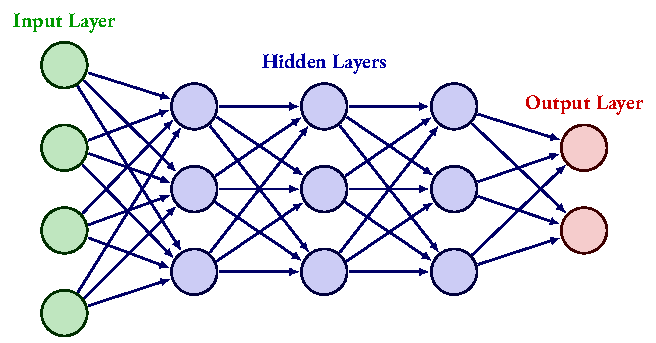
\includegraphics[scale=1.4]{tikz/chapter1 - Feedforward Neural Network.pdf}
    \caption{Example of a Feedforward Neural Network}
\end{figure}

A feedforward neural network can be thought of as a sequence of features, each of which represents a layer of the network. This structure is based on the composition of these functions to form an overall representation of the input data. Formally, we can represent a feedforward network as a composition of several functions:
$$ f(\mathbf{x}) = f^{(i)}(f^{(i-1)}(\dots f^{(2)}(f^{(1)}(\mathbf{x})) \dots )) $$  
Where \( f^{(1)} \) is the first layer (or input layer), \( f^{(i)} \) represents the output of the \(i\)-th layer, and so on. The depth of the network is defined by the number of layers, that is, the number of functions \( f^{(i)} \) involved.

In evaluating the functions of a feedforward network, which is acyclic graph, the flow of information proceeds in a single direction, from input to output. This flow passes through intermediate computations in the various layers of the network. 

In the initial layer, also called \textbf{\color{green!60!black}{Input Layer}}, each node corresponds to an input feature or variable, indeed there are no calculations or transformations applied to the data here.

Instead, neurons in the \textbf{\color{mybluee}{Hidden Layers}} perform nonlinear computations on the input data through the application of weights and activation functions.
The number of hidden layers and the number of neurons in each layer may vary depending on the architecture of the network and the complexity of the problem.
The main function of the hidden layers is to capture and represent complex and abstract features of the input data.

Finally in the \textbf{\color{red!80!black}{Output Layer}} we obtain the desired output.
The number of nodes in this layer depends on the nature of the problem, for example, in a binary classification problem there will be only one node, while in a multiclass classification problem there will be one node for each class.
Also the type of activation function used in the output layer depends on the type of problem the network is addressing! For example, for binary classification problems, the sigmoid activation function can be used, while for multiclass we use the softmax.

\subsection{Overcoming the limitations of linear models}

Linear models have long been used for their simplicity and convex optimization, but they have significant limitations in their ability to capture complex interactions between input variables. This limitation is particularly evident when dealing with complex problems such as nonlinear classification.

In the context of linear models, such as support vector machines, the choice of function \( \phi \) (\textbf{Nonlinear mapping of input data in feature space}) is crucial to satisfactory performance. However, there are limitations in engineering this function, which can make it difficult to capture complex information in the data. Below, we review three common options for addressing these challenges:
\begin{enumerate}
    \item \textbf{Use of generic \( \phi \)}: A first option is to use a generic \( \phi \) function. For example, in kernel machines with RBF (Radial Basis Function) kernels, \( \phi \) has implicit infinite dimensionality. This provides sufficient capacity to fit the training data. However, this approach may suffer from poor generalization for highly variable objective functions.
    \item \textbf{Engineer \( \phi \)}: Here, efforts are devoted to manually engineering a function that can capture the relevant information in the input data. However, this approach may be limited by the complexity of the data and the difficulty in correctly identifying key relationships.
    \item \textbf{Learning \( \phi \) from the data}: Finally, an option is to learn the \( \phi \) function directly from the data. This approach renounces convexity but offers significant advantages by combining the strengths of the first two options. \( \phi \) can be modeled very generically, and engineering can focus on designing neural network architectures capable of learning complex and informative representations from input data.
\end{enumerate}

Thanks to Feedforward Neural Networks we can overcome the limitations of traditional linear models because they are able to learn complex, nonlinear functions from data, thus overcoming the inherent limitations of linear models in capturing complex relationships between input variables.

The training of a neural network shares many similarities with that of other machine learning models. However, it has unique features that deserve to be explored. While it is essential to provide only the output of the final layers during training, the hidden layers do not require specific analysis during this phase, which contributes to the complexity and overall effectiveness of the network.

The main difference from linear models lies in the loss functions. While in linear models the loss is convex and guarantee convergence, in neural networks it become nonconvex, leading to greater complexity and not guaranteeing convergence to a global optimum.

Train a neural network means optimize the parameters' values $\mathbf{W}$ (wheights) in order to achieve $f(X,\mathbf{W})$ as close as the target unknown function $f(X)$. So, it is essential to apply gradient descent, an iterative approach to minimizing the cost function, and it is crucial to specify an appropriate \textbf{cost function} that accurately represents the error between the predicted output and the desired output. In addition, modeling choices may vary, including the selection of \textbf{output representation}, \textbf{activation functions}, and \textbf{network architecture} (e.g., number of layers), significantly affecting network performance.

Beyond that, there are other aspects of modeling that can be adapted to improve network performance, such as the choice of \textbf{optimizer} and the use of \textbf{regularization} techniques to avoid overfitting and improve generalization. 

To summarize, in a Neural Network we need to specify the following elements: cost function, output representation, activation function, architecture, optimizer, regularization.

\section{Cost Functions}

Cost (or Loss) functions play a key role in the training of deep learning models. They measure the \textbf{discrepancy between model predictions and actual target values} during the training process. An accurate choice of loss function is essential for optimal model performance.

For \textbf{Classification} problems, two commonly used loss functions are Categorical Cross-Entropy and Binary Cross-Entropy. These functions are designed to work with class probabilities and are particularly well suited for models that produce probability distributions.

{\Large
% $$
\begin{equation*}
\text{\textbf{Categorical Cross-Entropy}} = -\sum_{i=1}^{N} \tikzmarkk{Y}\textcolor{myred}{y_i} \log(\tikzmarkk{YC}\textcolor{mybluee}{\hat{y}_i})
\end{equation*}
\begin{tikzpicture}[overlay,remember picture]
    \node (Ye) [below of = Y, node distance = 3 em, anchor=west] {\footnotesize \textsf{\textcolor{myred}{true probability of class $i$}}};
    \draw[<-, in=180, out=-90] (Y.south)++(.25em,-1ex) to (Ye.west);

    \node (YCe) [below of = YC, node distance = 2 em, anchor=west] {\footnotesize \textsf{\textcolor{mybluee}{predicted probability of class $i$}}};
    \draw[<-, in=180, out=-90] (YC.south)++(.25em,-1ex) to (YCe.west);
\end{tikzpicture}
}

{\Large
% $$
\begin{equation*}
\text{\textbf{Binary Cross-Entropy}} = -\left(\tikzmarkk{Y}\textcolor{myred}{y}\log(\tikzmarkk{YC}\textcolor{mybluee}{\hat{y}}) + (1 - y) \log(1 - \hat{y})\right)
\end{equation*}
% $$
\begin{tikzpicture}[overlay,remember picture]
    \node (Ye) [below of = Y, node distance = 3 em, anchor=west] {\footnotesize \textsf{\textcolor{myred}{true label (0 or 1)}}};
    \draw[<-, in=180, out=-90] (Y.south)++(.25em,-1ex) to (Ye.west);

    \node (YCe) [below of = YC, node distance = 2 em, anchor=west] {\footnotesize \textsf{\textcolor{mybluee}{predicted probability of class 1}}};
    \draw[<-, in=180, out=-90] (YC.south)++(.25em,-1ex) to (YCe.west);
\end{tikzpicture}
}
\vspace{1cm}

In the case of \textbf{Regression}, different loss functions are used, including:

{\Large
% $$
\begin{equation*}
\text{\textbf{Mean Squared Error}} = \frac{1}{N} \sum_{i=1}^{N} (\tikzmarkk{Y}\textcolor{myred}{y_i} - \tikzmarkk{YC}\textcolor{mybluee}{\hat{y}_i})^2
\end{equation*}
% $$
\begin{tikzpicture}[overlay,remember picture]
    \node (Ye) [below of = Y, node distance = 3 em, anchor=west] {\footnotesize \textsf{\textcolor{myred}{actual (or true) target value for the example \( i \)}}};
    \draw[<-, in=180, out=-90] (Y.south)++(.25em,-1ex) to (Ye.west);

    \node (YCe) [below of = YC, node distance = 2 em, anchor=west] {\footnotesize \textsf{\textcolor{mybluee}{model prediction for the example \( i \)}}};
    \draw[<-, in=180, out=-90] (YC.south)++(.25em,-1ex) to (YCe.west);
\end{tikzpicture}
}
\vspace{1cm}

Mean Squared Error (MSE) calculates the mean squares of the differences between model predictions and actual values. It is commonly used and strongly penalizes significant errors. However, it is sensitive to outliers. 

% \newpage

{\Large
% $$
\begin{equation*}
\text{\textbf{Mean Absolute Error}} = \frac{1}{N} \sum_{i=1}^{N} |\tikzmarkk{Y}\textcolor{myred}{y_i} - \tikzmarkk{YC}\textcolor{mybluee}{\hat{y}_i}|
\end{equation*}
% $$
\begin{tikzpicture}[overlay,remember picture]
    \node (Ye) [below of = Y, node distance = 3 em, anchor=west] {\footnotesize \textsf{\textcolor{myred}{actual (or true) target value for the example \( i \)}}};
    \draw[<-, in=180, out=-90] (Y.south)++(.25em,-1ex) to (Ye.west);

    \node (YCe) [below of = YC, node distance = 2 em, anchor=west] {\footnotesize \textsf{\textcolor{mybluee}{model prediction for the example \( i \)}}};
    \draw[<-, in=180, out=-90] (YC.south)++(.25em,-1ex) to (YCe.west);
\end{tikzpicture}
}
\vspace{1cm}

Mean Absolute Error (MAE), or only Absolute Error (AE), calculates the mean of the absolute differences between predictions and actual values. It is less sensitive to outliers than MSE, but its derivative is undefined in zero.

{\Large
% $$
\begin{equation*}
\text{\textbf{Huber Loss}} = \frac{1}{N} \sum_{i=1}^{N} \left\{
\begin{array}{ll}
    \frac{1}{2} (y_i - \hat{y}_i)^2 & \text{se } |y_i - \hat{y}_i| \leq \textcolor{mygreen}{\delta} \\
    \tikzmarkk{D}\textcolor{mygreen}{\delta} (|y_i - \hat{y}_i| - \frac{1}{2} \textcolor{mygreen}{\delta}) & \text{otherwise}
\end{array}
\right.
\end{equation*}
% $$
\begin{tikzpicture}[overlay,remember picture]
    \node (De) [below of = D, node distance = 2.5 em, anchor=west]     {\parbox{\widthof{hyperparameter controlling the transition between}}{
    \ \\
    \footnotesize \textsf{\textcolor{mygreen}{hyperparameter controlling the transition between}} \\ 
    \footnotesize \textsf{\textcolor{mygreen}{the quadratic and linear regions of the loss function}}}};
    \draw[<-, in=180, out=-90] (D.south)++(.25em,-.5ex) to (De.west);
\end{tikzpicture}
}
\vspace{1cm}

Huber Loss combines the best features of MSE and MAE. For small errors, it behaves similar to MSE, while for larger errors, it behaves like AE. This avoids problems such as overfitting and steep slope of the MSE curve.

\textit{\textbf{Please Note}}: There are numerous other loss functions besides those mentioned above, which can be used depending on the specific problem to be addressed and the characteristics of the data. The choice of loss function depends on the goal of model training, the nature of the data, and the needs of the application. For example, in special contexts such as outlier detection or handling noisy data, specialized loss functions might be preferred. Moreover, as deep learning research advances, new loss functions are constantly being developed and existing ones adapted to meet emerging challenges in different application scenarios. 

\textit{\textbf{Also}}: The choice of the cost function is not independent of the choice of the output unit, because choosing one specific output unit over another can be convenient for the cost function we want to use (e.g., sigmoid and binary cross-entropy).

\section{Unit Types}

\subsection{Linear Units}

Linear Units play a key role in the intermediate and output layers of neural networks. These units apply a \textbf{linear transformation to the inputs} by combining the weights associated with the inputs with the input values themselves. The output produced by Linear Units is a linear combination of the inputs. 

The formula for calculating the output of Linear Units is:
$$
\hat{y} = W^T h + b
$$
Where \( \hat{y} \) represents the predicted output, \( W \) are the weights associated with the inputs, \( h \) represents the features from the previous layer, and \( b \) is the bias term.

\subsection{Softmax Units}

Softmax Units are commonly used in the output layers of neural networks, especially in cases of Multiclass Classification (with Cross-Entropy Loss). These units transform the un-normalized scores from the last linear layer into a \textbf{normalized probability distribution}, allowing the model to assign a probability to each membership class for a given input.

The softmax formula used to calculate the probabilities is as follows:
$$
\text{Softmax}(z_i) = \frac{e^{z_i}}{\sum_{j} e^{z_j}}
$$
Where \( z_i \) represents the non-normalized score associated with the class \( i \), and \( \sum_{j} e^{z_j} \) is the sum of all the exponents of the non-normalized scores.

Log Softmax is a variant of the Softmax function that is used to \textbf{improve numerical stability} when computing probabilities. The formula for calculating the Log Softmax is as follows:
$$
\text{log Softmax}(z_i) = z_i - \log\left(\sum_{j} e^{z_j}\right)
$$

Here are some advantages:
\begin{itemize}
    \item \textbf{The term \( z_i \) never saturates}: This means that the scale of values \( z_i \) is not compressed or restricted in any way. This is beneficial because it allows the model to continue to learn from more relevant information without limitations imposed by value saturation.
    
    \item \textbf{Maximizing the log-likelihood encourages \( z_i \) to be increased, while encouraging all other \( z \) to be decreased}: When we maximize the log-likelihood, we are trying to make the model's prediction as close to reality as possible. Thus, we encourage \( z_i \) to increase, since it represents the probability associated with the correct class. At the same time, we encourage the other \( z \) to decrease to reduce the probability associated with the wrong classes.
    
    \item \textbf{The log-likelihood cost function heavily penalizes the most active incorrect prediction}: The log-likelihood cost function significantly penalizes the most active incorrect prediction. This means that if the model is very sure of an incorrect prediction (for example, it has a very high probability for an incorrect class), the cost function will increase significantly, encouraging the model to correct that error.
\end{itemize}

This analysis prompts us to consider a fundamental question: \textit{How can we select the activation function $h$ most suitable for our neural network?}

In the next section, we try to answer this crucial question! 
We have decided to be quite descriptive, as we believe that more details about these functions can facilitate a deeper understanding.

\section{Activation Functions}

\subsection{Sigmoid}

\begin{table}[h]
\begin{tabularx}{\linewidth}{>{\parskip1ex}X@{\kern4\tabcolsep}>{\parskip1ex}X}
\toprule
\hfil\bfseries \color{mybluee}{Pros}
&
\hfil\bfseries \color{mybluee}{Cons}
\\\cmidrule(r{3\tabcolsep}){1-1}\cmidrule(l{-\tabcolsep}){2-2}

%% PROS
The sigmoid function offers a valuable advantage because it acts as a type of \textbf{\textcolor{mybluee}{squashing non-linearity}} that "squeezes" outputs within the range of [$0$, $1$]. This feature is particularly advantageous in scenarios such as binary classification tasks, where the model must generate outputs that can be interpreted as probabilities.

Moreover, the sigmoid function has a property of \textbf{\textcolor{mybluee}{differentiability and smoothness}} over its entire domain. This property facilitates seamless integration with gradient-based optimization techniques, ensuring stable convergence during the training process.
&

%% CONS
However, it \textbf{\textcolor{mybluee}{tends to saturate}} in most of its domain. This saturation phenomenon causes the gradient to tend toward zero, posing challenges during the learning phase. Consequently, this saturation can obstruct the effective propagation of gradients through the network during back-propagation.

In addition, the sigmoid function shows strong sensitivity mainly when the input is near zero. In contrast, its \textbf{\textcolor{mybluee}{sensitivity decreases}} for both large and small input values. This characteristic negatively affects the model's ability to learn from datasets that have a wide range of input values.
\\\bottomrule
\end{tabularx}
\caption{Benefits and Limitations of Sigmoid Activation}
\end{table}

\vspace{1cm}
\begin{figure}[!htbp]
    \centering
    \includegraphics[scale=2]{tikz/chapter1 - Sigmoid.pdf}
    \caption{Sigmoid Activation Function Plot}
\end{figure}

\newpage
\subsection{Hyperbolic Tangent}

\begin{table}[h]
\begin{tabularx}{\linewidth}{>{\parskip1ex}X@{\kern4\tabcolsep}>{\parskip1ex}X}
\toprule
\hfil\bfseries \color{myred}{Pros}
&
\hfil\bfseries \color{myred}{Cons}
\\\cmidrule(r{3\tabcolsep}){1-1}\cmidrule(l{-\tabcolsep}){2-2}

%% PROS
First, it is \textbf{\textcolor{myred}{differentiable and continuous}}, ensuring compatibility with gradient-based optimization techniques. 

In addition, the hyperbolic tangent function is \textbf{\textcolor{myred}{similar to sigmoid}}, but provides a more favorable output range. By squashing the outputs in the interval [$-1$, $1$], it ensures that the outputs are centered in zero. This feature can improve the model's ability to learn and adapt to data distributions, especially in scenarios where centered data is advantageous.
&

%% CONS
However, the hyperbolic tangent function also has limitations. Like the sigmoid, it tends to \textbf{\textcolor{myred}{saturate}} throughout much of its domain. This saturation phenomenon can hinder effective gradient propagation during back-propagation, impeding the learning process and potentially leading to slower convergence.
\\\bottomrule
\end{tabularx}
\caption{Benefits and Limitations of Hyperbolic Tangent Activation}
\end{table}

\vspace{1cm}
\begin{figure}[!htbp]
    \centering
    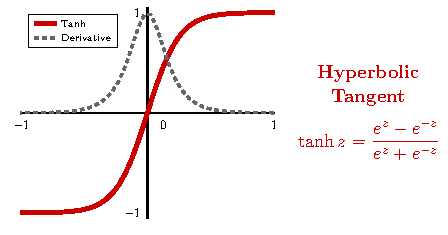
\includegraphics[scale=2]{tikz/chapter1 - Hyperbolic Tangent.pdf}
    \caption{Hyperbolic Tangent Activation Function Plot}
\end{figure}

\newpage
\subsection{Rectified Linear Unit (ReLU)}
\begin{table}[h]
\begin{tabularx}{\linewidth}{>{\parskip1ex}X@{\kern4\tabcolsep}>{\parskip1ex}X}
\toprule
\hfil\bfseries \color{mygreen!80!black}{Pros}
&
\hfil\bfseries \color{mygreen!80!black}{Cons}
\\\cmidrule(r{3\tabcolsep}){1-1}\cmidrule(l{-\tabcolsep}){2-2}

%% PROS
The ReLU function has several advantages. First, it provides \textbf{\textcolor{mygreen!80!black}{wide and consistent gradients}} when it is active. This means that the ReLU function does not saturate when it is active, which greatly accelerates the convergence of gradient-based optimization.
In addition, the \textbf{\textcolor{mygreen!80!black}{non-positive limitation}} accelerates the convergence of gradient descent, allowing for faster learning.
The ReLU function may have a limitation in its \textbf{\textcolor{mygreen!80!black}{differentiability}}. However, in practice, this is not necessarily a problem since the one-sided derivative is returned when \( z = 0 \). Moreover, gradient-based optimization is subject to numerical errors anyway, so this differentiability limitation is often overlooked.
A good practice is to \textbf{\textcolor{mygreen!80!black}{initialize bias}} with small positive values. This ensures that units are initially active for most inputs and that derivatives can propagate through.
&

%% CONS
However, the ReLU function also has some disadvantages. First of all, its outputs are not \textbf{\textcolor{mygreen!80!black}{centered on zero}}, which could cause problems in some machine learning contexts.
In addition, ReLU neurons may suffer from a phenomenon called \textbf{\textcolor{mygreen!80!black}{"dying ReLU"}}. This occurs when most of the inputs to ReLU neurons are in the negative range. When this occurs, the ReLU neurons return an output of $0$ and the gradients do not flow during back-propagation, preventing the weights from updating. However, this problem does not always occur and can be mitigated by properly adjusting the learning rate or using Stochastic Gradient Descent (SDG).
The ReLU function can also be sensitive to the \textbf{\textcolor{mygreen!80!black}{large learning rate}}. If the learning rate is too high, the new weights are likely to end up in the highly negative range, negatively affecting the convergence of the model.
\\\bottomrule
\end{tabularx}
\caption{Benefits and Limitations of ReLU Activation}
\end{table}

\vspace{1cm}
\begin{figure}[!htbp]
    \centering
    \includegraphics[scale=2]{tikz/chapter1 - ReLU.pdf}
    \caption{ReLU Activation Function Plot}
\end{figure}


\subsection{Generalized Rectified Linear Units}

The \textbf{generalized rectified linear units} were introduced to address some limitations of the ReLU function. The main objective is to obtain a non-zero slope when \( z_i < 0 \). The generalized form of the ReLU is defined as follows:
$$ h(z, \alpha_i) = \max(0, z_i) + \alpha_i \min(0, z_i) $$
However, generalized rectified linear units are not universally better than ReLU and may lead to other problems, such as additional computational complexity. Some of the improvements that have been made include:
\begin{itemize}     
    \item \textbf{Leaky ReLU}: This variation solves the problem of neuron death by setting \( a_i \) to a small value, such as $0.01$, to maintain a gradient flow even when the input is negative.
    \item \textbf{Parametric ReLU}: This variant allows the parameter \( a_i \) to be learned, allowing the network to adapt the gradient of the activation function based on the data.
    \item \textbf{ReLU Randomized}: This variant samples the parameter \( a_i \) from a fixed interval during training and keeps it constant during testing, introducing randomness into the model.
\end{itemize}

In addition, other activation functions have been proposed as alternatives to ReLU, including:
\begin{itemize}     
    \item \textbf{Exponential Linear Units (ELU)}: This activation function retains all the advantages of ReLU but avoids the problem of neuron death. However, it requires exponentiation during computation, slightly increasing the computational complexity.
    \item \textbf{Swish}: This function is a smooth, non-monotonic function that has been shown to perform better than ReLU on deeper models, improving performance on datasets such as ImageNet.
    \item \textbf{Linear Units with Gaussian Error (GELU)}: This activation function has been used in state-of-the-art algorithms such as GPT-3 and BERT. It combines the non-monotonic aspect (that helps for the gradient of the function),  regularization techniques such as dropout and zone-out, and ReLU benefits to achieve a smoother version of ReLU. 
\end{itemize}

% These improvements and generalizations of activation functions have helped make neural networks more efficient and adaptable to a wide range of machine learning problems. Below, we show graphs of the Leaky ReLU and ELU activation functions for a better understanding of their properties.

\begin{figure}[!htbp]
    \centering
    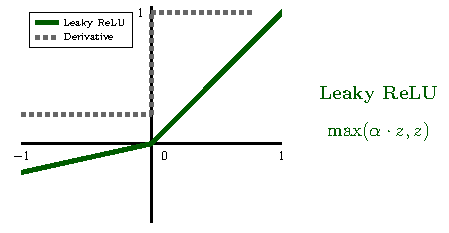
\includegraphics[scale=2]{tikz/chapter1 - Leaky ReLU.pdf}
    \caption{Leaky ReLU Activation Function Plot}
\end{figure}

\begin{figure}[!htbp]
    \centering
    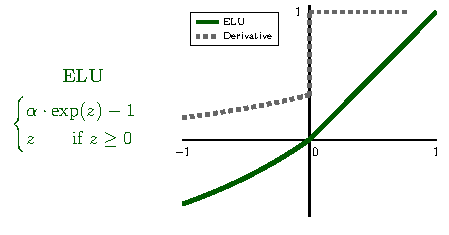
\includegraphics[scale=2]{tikz/chapter1 - ELU.pdf}
    \caption{ELU Activation Function Plot}
\end{figure}

\section{Architecture design}
\textit{How do we decide depth and width?} Choosing the depth and width of a neural network depends on several factors, including the complexity of the problem to be solved, the availability of training data, and the computational resources available. In principle, how many hidden layer units are sufficient? Theory offers us some answers.

\begin{remark}
Cybenko's Theorem (1989), also known as the universal approximation theorem, states that \textbf{a two-layer neural network with linear output can approximate any continuous function} over a compact domain with arbitrary precision, provided there are enough hidden units. This theorem has important implications for the design of neural architectures.
\end{remark}

\textbf{Implications}: Regardless of the function we are trying to learn, we know that a large multilayer neural network can represent this function. However, there is no guarantee that our training algorithm will be able to learn that function, due to optimization or data overlap issues. Also, the theorem gives no indication of how large the network will be.

\textit{So is depth or width more important?} There are trade-offs between depth and width of neural networks. For example, deeper networks generally generalize better: imagine a neural network as a set of tools to solve a problem. The more tools you have, the more complex problems you can solve. Then, by adding more "layers" to the network (making it deeper), we could give the network the ability to tackle more difficult problems or capture finer details in the data. In addition, architecture design has a significant impact on performance, for example between convolutional and feedforward neural networks.

\newpage
\chapter{Backpropagation} 
\setbackgroundchapter{Backpropagation}
\section{The Gradient Descent Algorithm}

\vspace{-0.4cm}
To train neural networks effectively, we employ the (Stochastic) \textbf{Gradient Descent algorithm} in combination with \textbf{Backpropagation}. Backpropagation, a method for computing gradients, is crucial for updating the parameters of the neural network during training. We will delve into it shortly, but first, let's explore Gradient Descent and its significance.
\vspace{-0.4cm}

\subsection{Understanding the Gradient}

Gradient Descent is a fundamental optimization algorithm used to minimize the loss function of a neural network by iteratively adjusting its parameters. The goal is to find the optimal set of parameters that result in the lowest possible loss. The algorithm works by iteratively moving in the \textbf{direction of the steepest descent of the loss function} with respect to the parameters. This direction is determined by the \textbf{negative gradient} of the loss function, which is why we will utilize the negative sign in the algorithm.

Mathematically, the update rule for the parameters \( w \) in Gradient Descent can be expressed as:
$$
\Delta_w L = \left[ \frac{\partial L}{\partial w_1}, \frac{\partial L}{\partial w_2}, \ldots , \frac{\partial L}{\partial w_N}\right]
$$
where \( \Delta_w L \) represents the change in the loss function \( L \) with respect to the parameters \( w \), and \( \frac{\partial L}{\partial w_i} \) denotes the partial derivative of the loss function with respect to the \( i \)-th parameter \( w_i \).

Below we show a figure illustrating the partial derivatives of a function. The figure is represented in two ways: in a 3D graph and in the two-dimensional projection of the same graph (top view). The surface of the graph represents the function, where the lowest point is colored blue and the highest point is colored red. The black arrows extending from the surface indicate the direction and intensity of the gradient change of the function at each point in space. This visualization is crucial for understanding how Gradient Descent finds the fastest direction to reduce loss and update model weights during neural network training.

\begin{figure}[!htbp]
    \centering
    \includegraphics[scale=2]{tikz/chapter2 - Partial Derivatives.pdf}
    \caption{Visualization of Partial Derivatives in Two Distinct Ways}
\end{figure}

Having understood partial derivatives and the role of the gradient in the optimization process, let's now look at a visual representation of how the Gradient Descent algorithm works. In the image below, we see a three-dimensional surface representing the loss function. As before, the lowest point of the surface is colored blue and represents the minimum of the loss function. The black arrows extending from the surface indicate the \textbf{path} that Gradient Descent follows \textbf{to reach the minimum}. Each arrow represents the direction and intensity of the change in the loss function at a given point in space.

\begin{figure}[!htbp]
    \centering
    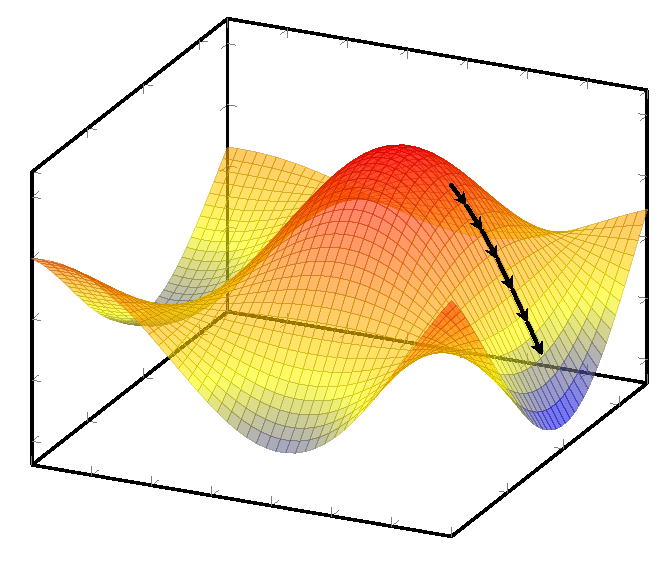
\includegraphics[scale=0.75]{tikz/chapter2 - Gradient Descent.pdf}
    \caption{Visual Representation of the Gradient Descent Algorithm}
\end{figure}

The algorithm proceeds by iteratively updating the parameters according to the gradient direction \textbf{until convergence is reached or a predefined number of iterations is completed}. By following this process, Gradient Descent effectively navigates the parameter space to find the optimal configuration that minimizes the loss function.


\subsection{The Problem of Local Minima}

In neural networks, the optimization problem is non-convex, leading to the existence of \textbf{local minima}. However, practitioners have found that these local minima are often still effective solutions. Thus, local minima are not typically a significant concern in neural network training. Below, we show an example illustrating the local minima problem for a better insight.

\begin{figure}[!htbp]
    \centering
    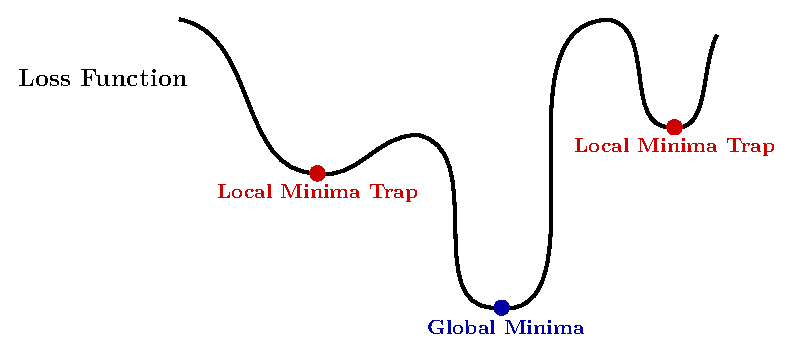
\includegraphics[scale=0.9]{tikz/chapter2 - Local Minima.pdf}
    \caption{Local and Global Minima}
\end{figure}

\subsection{The Problem of Sad\partial Le Points}

Another optimization challenge arises from sad\partial Le points, where some directions curve upwards and others downwards. At a sad\partial Le point, the \textbf{gradient is zero}, even if the point is not a minimum. Sad\partial Le points are common in high-dimensional spaces. However, they only become problematic if the optimization algorithm becomes stuck exactly at the sad\partial Le point.

\begin{figure}[!htbp]
    \centering
    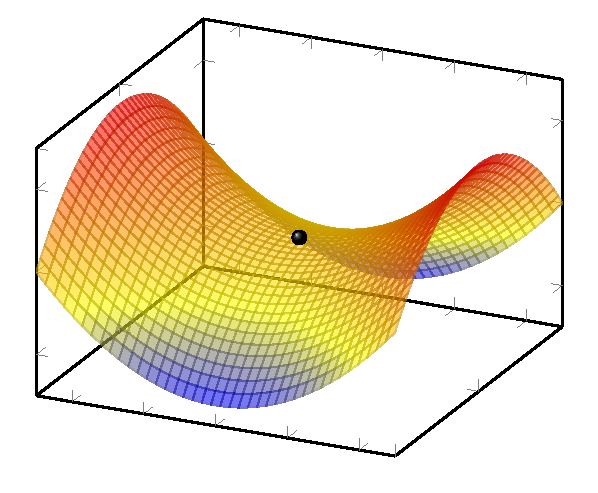
\includegraphics[scale=0.88]{tikz/chapter2 - Saddle Point.pdf}
    \caption{Saddle Le Point Illustration}
\end{figure}

In the figure, there is a saddle point depicted within the neural network optimization scenario, represented by the black dot. 

\section{Backpropagation Algorithm}

\subsection{Backpropagation Fundamentals}
How do we learn the weights of a neural network? Let us examine some ideas that have guided the development of learning algorithms in the context of neural networks.

The initial idea was to \textbf{randomly perturb one weight at a time}, evaluating whether that change improved model performance and saving the change. This approach, although similar to an evolutionary process, proved to be very inefficient, requiring numerous passes over the training data for each change in the weights and presenting difficulties in the last stage of learning.

Another idea involved \textbf{perturbing all the weights simultaneously} and correlating performance improvement with changes in the weights. However, this method proved equally inefficient and extremely difficult to implement.

Subsequently, a more efficient idea was proposed: to \textbf{perturb only the activations}, which are fewer in number than the weights. Although this approach is an improvement over the previous ones, it is still inefficient.

\textit{Therefore, how can we achieve more efficient learning?} This is where backpropagation comes in.

\begin{remark}
Backpropagation is a widely used learning algorithm in neural networks, which consists of three main steps:

\begin{enumerate}
    \item \textbf{Forward Propagation}: summation of inputs, production of activations and propagation of output through the network.

    \item \textbf{Error Estimation}: comparison of labels with predictions obtained from the network.

    \item \textbf{Backpropagation} of the error signal and using this signal to update the weights by computing gradients.
\end{enumerate}
\end{remark}

Starting from the training data, we do not directly know the optimal behavior of the hidden units within the neural network. However, using backpropagation, we can calculate how quickly the overall error of the network changes when we change the activity of these hidden units.

Using the derivatives of the error with respect to the hidden activities, we are able to understand \textbf{how each hidden unit affects the overall error of the network}. This allows us to gain a clear view of the separate effects that each hidden unit has on the error and how these effects are combined to determine the optimal direction to update the network weights.

Once we have calculated the derivatives of the error with respect to the hidden activities, we gain valuable information to update the weights associated with each connection in the network. This allows us to adjust the weights in a way that minimizes the overall error in the network, moving us closer and closer to the optimal solution for the learning problem.

\section{Exploring Backpropagation: Step by Step}

In this section, we will explore backpropagation of the error through a neural network in detail, starting with the output layer and proceeding to the input layer. We begin with a neural network composed of \textbf{one neuron per layer}.

\begin{minipage}{0.45\textwidth}
\includegraphics[width=\textwidth]{tikz/chapter2 - Chain Rule One Layer.pdf}
\captionof{figure}{Conceptualisation of Calculations}
\end{minipage}
\begin{minipage}{0.55\textwidth}
After performing the forward step, we will get an output from the last activation \( a^{(l)} \), which will allow us to calculate the loss \( \textcolor{myred}{L} \) using the desired output \( y \). The latter activation \( a^{(l)} \) is calculated using three elements: a weight \( \textcolor{myblue}{w^{(l)}} \), a bias \( \textcolor{myorange}{b^{(l)}} \), and the activation of the preceding neuron \( a^{(l-1)} \). The resulting equations are as follows:

$$ \textcolor{mygreen}{z^{(l)}} = \textcolor{myblue}{w^{(l)}} a^{(l-1)} + \textcolor{myorange}{b^{(l)}} $$
$$ a^{(l)} = \sigma(\textcolor{mygreen}{z^{(l)}}) $$
Where \textcolor{mygreen}{$z^{(l)}$} is the input of a non-linear function $\sigma$, such as a sigmoid or a ReLU. \\

A way you might conceptualize this is that the weight \( \textcolor{myblue}{w^{(l)}} \), the prior activation \( a^{(l-1)} \), and the bias \( \textcolor{myorange}{b^{(l)}} \) together \textbf{\textcolor{myyellow!85!black}{allow us to calculate}} \( \textcolor{mygreen}{z^{(l)}} \), which in turn \textbf{\textcolor{myyellow!85!black}{allow us to calculate}} \( a^{(l)} \), which together with the desired output \( y \) \textbf{\textcolor{myyellow!85!black}{allows us to calculate the loss}} \( \textcolor{myred}{L} \). This concept is illustrated in the diagram on the left.
\end{minipage}

Our initial goal during the backward step is to understand how sensitive the loss \( \textcolor{myred}{L} \) is to small changes in the weight \( \textcolor{myblue}{w^{(l)}} \), that is, calculate the derivative\( \frac{\textcolor{myred}{\partial L}}{\textcolor{myblue}{\partial w^{(l)}}} \). 
Conceptually, when you see this kind of formula, we need to think of it as saying to us "\textbf{how much does \( \textcolor{myred}{L} \) (numerator) change if we make a small change at \( \textcolor{myblue}{w^{(l)}} \) (denominator)?}"

When we calculate this derivative, we note that a small change in weight \( \textcolor{myblue}{w^{(l)}}\) \textbf{\textcolor{myyellow!85!black}{causes a change in}} \( \textcolor{mygreen}{z^{(l)}} \), which in turn \textbf{\textcolor{myyellow!85!black}{causes a change in}} \( a^{(l)} \), \textbf{\textcolor{myyellow!85!black}{directly affecting}} the loss \( \textcolor{myred}{L} \). And so this is where the chain of derivatives rule comes into play! 

As can be seen below we can now "chunk" the previous derivative:

\vspace{-0.8cm}
{\Large
% $$
\begin{equation*}
\hspace*{1cm}
\frac{\textcolor{myred}{\partial L}}{\textcolor{myblue}{\partial w^{(l)}}} = \frac{\textcolor{mygreen}{\partial z^{(l)}}}{\textcolor{myblue}{\partial \tikzmarkk{Z}w^{(l)}}}  
\frac{\partial a^{(l)}}{\textcolor{mygreen}{\partial \tikzmarkk{Y}z^{(l)}}} \frac{\textcolor{myred}{\partial L}}{\partial \tikzmarkk{YC}a^{(l)}}
\end{equation*}
% $$
\begin{tikzpicture}[overlay,remember picture]
    \node (Ze) [below of = Z, node distance = 4 em, anchor=west] {\footnotesize How much does a little variation to \( \textcolor{myblue}{w^{(l)}} \) changes \( \textcolor{mygreen}{z^{(l)}} \)?};
    \draw[<-, in=180, out=-90] (Z.south)++(.25em,-1ex) to (Ze.west);

    \node (Ye) [below of = Y, node distance = 3 em, anchor=west] {\footnotesize How much does a little variation to \( \textcolor{mygreen}{z^{(l)}} \) changes \( a^{(l)} \)?};
    \draw[<-, in=180, out=-90] (Y.south)++(.25em,-1ex) to (Ye.west);

    \node (YCe) [below of = YC, node distance = 2 em, anchor=west] {\footnotesize How much does a little variation to \( a^{(l)} \) changes \( \textcolor{myred}{L} \)?};
    \draw[<-, in=180, out=-90] (YC.south)++(.25em,-1ex) to (YCe.west);
\end{tikzpicture}
}
\vspace{1.8cm}

\textit{What about the bias term? Easy peasy!} We use the same method as for the weight term:

\vspace{-0.3cm}
$$\frac{\textcolor{myred}{\partial L}}{\textcolor{myorange}{\partial b^{(l)}}} = \frac{\textcolor{mygreen}{\partial z^{(l)}}}{\textcolor{myorange}{\partial b^{(l)}}}  \frac{\partial a^{(l)}}{\textcolor{mygreen}{\partial z^{(l)}}} \frac{\textcolor{myred}{\partial L}}{\partial a^{(l)}}$$

\textit{Now what? For the other layers?} Let's go back to our scheme for a moment and extend it:

\begin{figure}[htbp]
\centering
\includegraphics[width=\textwidth]{tikz/chapter2 - Chain Rule Multiple Layer.pdf}
\caption{Conceptualisation of Calculations (Extended)}
\end{figure}

All other weights and biases are in the earlier layers of the network, which means that their influence on cost is less direct. The way we han\partial Le them is to first consider how sensitive the cost is to the value of that activation in the penultimate layer, \( a^{(l-1)} \), and then consider how sensitive that value is to all the previous weights and biases.

The derivative of cost with respect to that activation looks a lot like what we have already seen:

\vspace{-0.5cm}
$$\frac{\textcolor{myred}{\partial L}}{\partial a^{(l-1)}} = \frac{\textcolor{mygreen}{\partial z^{(l)}}}{\partial a^{(l-1)}}  \frac{\partial a^{(l)}}{\textcolor{mygreen}{\partial z^{(l)}}} \frac{\textcolor{myred}{\partial L}}{\partial a^{(l)}}$$

The trick here is to remember that the activation in the previous layer is determined by its set of weights and biases. For example, there is a long chain of dependencies between the weight \( w^{(l-1)} \) and the cost \( \textcolor{myred}{L} \). The way this presents itself mathematically is that the partial derivative of the cost with respect to that weight appears as a long chain of partial derivatives for each intermediate step, see the image below to visualize the concept graphically.

\begin{minipage}{0.55\textwidth}

Here is how you can decompose the derivative:

\vspace{-0.3cm}
$$\frac{\textcolor{myred}{\partial L}}{\textcolor{myblue}{\partial w^{(l-1)}}} = 
\frac{\textcolor{mygreen}{\partial z^{(l-1)}}}{\textcolor{myblue}{\partial w^{(l-1)}}}  
\frac{\partial a^{(l-1)}}{\textcolor{mygreen}{\partial z^{(l-1)}}} 
\underbrace{
\frac{\textcolor{mygreen}{\partial z^{(l)}}}{\textcolor{myblue}{\partial w^{(l)}}}  
\frac{\partial a^{(l)}}{\textcolor{mygreen}{\partial z^{(l)}}} 
\frac{\textcolor{myred}{\partial L}}{\partial a^{(l)}}}_\textrm{\Large$\frac{\textcolor{myred}{\partial L}}{\textcolor{myblue}{\partial w^{(l)}}}$}$$
\vspace{-0.3cm}
\ \\
By following the dependencies through our tree and multiplying together a long series of partial derivatives, we now \textbf{can calculate the derivative of the cost with respect to any weight or bias of the entire network}. \textit{We are simply applying the same idea of the chain rule that we have always used!} \\

And since we can get any derivative, we can calculate the entire gradient vector:
\vspace{-0.1cm}
$$
\Delta_w L = \left[ \frac{\textcolor{myred}{\partial L}}{\textcolor{myblue}{\partial w^{(1)}}}, \frac{\textcolor{myred}{\partial L}}{\textcolor{myorange}{\partial b^{(1)}}}, \ldots , \frac{\textcolor{myred}{\partial L}}{\textcolor{myblue}{\partial w^{(l)}}}, \frac{\textcolor{myred}{\partial L}}{\textcolor{myorange}{\partial b^{(l)}}},\right] 
$$
\vspace{-0.3cm}
\ \\
The job is done! At least for this network, now we must add more neurons for each layer. \textit{I know, you are crying inside, but actually, not much changes when we give the layers more neurons: it's just a few more indexes to keep track of \emoji{smile}}.

\vspace{1cm}

\end{minipage}
\begin{minipage}{0.45\textwidth}
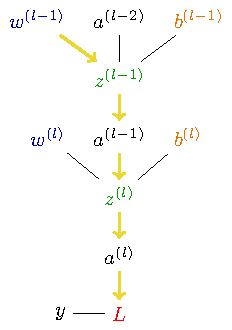
\includegraphics[width=\textwidth]{tikz/chapter2 - Chain Rule Multiple Layer Dependencies.pdf}
\captionof{figure}{Calculations with 3 Layers}
\end{minipage}

\begin{minipage}{0.4\textwidth}
\includegraphics[width=\textwidth]{tikz/chapter2 - Indexing.pdf}
\captionof{figure}{Neural Network Indexing}
\vspace{0.8cm}
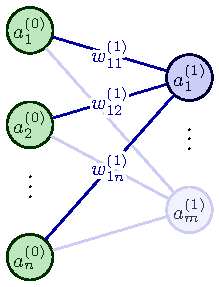
\includegraphics[width=\textwidth]{tikz/chapter2 - Indexing Example.pdf}
\captionof{figure}{Example of Indexing}
\end{minipage}
\begin{minipage}{0.05\textwidth}
\
\end{minipage}
\begin{minipage}{0.55\textwidth}
When dealing with neural networks with multiple neurons per layer, we have to change the notations a bit.\\

The activation of each neuron will be denoted with a subscript indicating its position within the layer. Thus, \textbf{the superscript of each neuron indicates which layer it is in, while the subscript indicates the specific neuron}.\\

The weights also need a refresh: additional indices are required to specify their location. In addition to the superscript representing the layer, \textbf{two subscripts indicate the edge weight connecting the neuron in layer $i$ to the neuron in layer $j$}.\\

\textit{I know, these "$ji$" indices, being backwards, might seem strange or unconventional at first, but they align with the way the weight matrix is usually indexed.}\\

On the left are two images: one formally represents how the nodes and edges of the network are represented, while the other provides an example with two dummy layers, named $0$ and $1$, with $n$ and $m$ nodes, respectively.
\end{minipage}

\newpage
The weighted sum \textcolor{mygreen}{$z_{j}^{(l)}$} then takes the following form:
$$
\textcolor{mygreen}{z_{j}^{(l)}} = \sum_{i} \textcolor{myblue}{w_{ji}^{(l)}} \cdot a_i^{(l-1)} + \textcolor{myorange}{b_{j}^{(l)}}
$$
The new equations turn out to be esentially the same with respect to the case of only one neuron per layer:

\vspace{-0.4cm}
$$
\frac{\textcolor{myred}{\partial L}}{\textcolor{myblue}{\partial w_{ji}^{(l)}}} = \frac{\textcolor{mygreen}{\partial z_{j}^{(l)}}}{\textcolor{myblue}{\partial w_{ji}^{(l)}}}  
\frac{\partial a_{j}^{(l)}}{\textcolor{mygreen}{\partial z_{j}^{(l)}}} \frac{\textcolor{myred}{\partial L}}{\partial a_{j}^{(l)}}
$$

Indeed, the expression of the derivative of the chain rule describing the sensitivity of cost with respect to a particular weight is the same as in the previous case. The only difference is that we now have multiple indices, $i$ and $j$, indicating which weight we are considering.

What changes, however, is the derivative of the cost with respect to one of the activations in the preceding layers, because \textbf{the preceding neurons influence the cost function through multiple pathways}.

To understand the sensitivity of the cost function with respect to a certain neuron, it is necessary to sum the influences along each of these different pathways. So, we \textbf{sum multiple expressions of different chain rules corresponding to each pathway of influence}.

\vspace{-0.5cm}
$$\frac{\textcolor{myred}{\partial L}}{\partial a_{i}^{(l-1)}} = \underbrace{\sum_{j}\frac{\textcolor{mygreen}{\partial z_{j}^{(l)}}}{\partial a_{i}^{(l-1)}}  \frac{\partial a_{j}^{(l)}}{\textcolor{mygreen}{\partial z_{j}^{(l)}}} \frac{\textcolor{myred}{\partial L}}{\partial a_{j}^{(l)}}}_\textrm{Sum over layer $l$}$$

This reasoning is carried out using traditional numerical values, but it is evident that in order to efficiently handle the weights and biases of the neural network, it is necessary to use the \textbf{matrix approach}, since it allows simultaneous operations to be performed on all the parameters of the network, greatly optimizing the computational process.


\newpage
\chapter{Optimization}
\setbackgroundchapter{Optimization}
\vspace{-0.4cm}
In this chapter, we will immerse ourselves in optimization, exploring a wide range of gradient descent algorithms. We will start from the classic batch gradient descent to more advanced ones such as ADAM. But optimization does not stop there: we will also introduce a crucial element, data normalization, which contributes significantly to the effectiveness of our models. \textit{Ready to explore the nitty-gritty of these techniques? Let's dive in!}
\vspace{-0.4cm}

\section{Types of Gradient Descent}

\subsection{Batch Gradient Descent (BGD)}

The Batch Gradient Descent algorithm is one of the most widely used methods for parameter optimization in a neural network. Below we provide the algorithm.

\begin{algorithm}
\renewcommand\thealgorithm{}
\caption{\textbf{\textcolor{mygreen}{Batch Gradient Descent}}}
\begin{algorithmic}[1]
\REQUIRE{Learning Rate $\varepsilon$}
\REQUIRE{Initial Parameters $\mathbf{w}$}
\WHILE{Stopping Criteria not met}
    \STATE Compute gradient estimate on \textbf{\textcolor{myred}{$\mathbf{N}$ training examples}} $\{ (\mathbf{x}^{(1)}, y^{(1)}), ..., (\mathbf{x}^{(N)}, y^{(N)}) \}$
    \STATE $
    \mathbf{\hat{g}} \leftarrow \frac{1}{N}\nabla_{\mathbf{w}} \sum_{i=1}^{N} L(f(\mathbf{x}^{(i)},\mathbf{w}), y^{(i)})
    $
    \STATE Update parameters:
    $
    \textcolor{mybluee}{\mathbf{w} \leftarrow \mathbf{w} - \varepsilon \mathbf{\hat{g}}} 
    $
\ENDWHILE
\end{algorithmic}
\end{algorithm}

The distinguishing feature of Batch Gradient Descent is that it uses the \textbf{\textcolor{myred}{entire training dataset to calculate the gradient}} of the loss function. This means it requires \textbf{more computational resources and computation time} than other methods, but it can also lead to \textbf{more stable and accurate convergence}.
Therefore, Batch Gradient Descent remains one of the most widely used algorithms for training neural networks due to its conceptual simplicity and its effectiveness in learning model parameters. 

\subsection{Stochastic Gradient Descent (SGD)}

The Stochastic Gradient Descent algorithm, on the other hand, computes and applies parameter updates for each individual training example rather than using the entire training dataset. Below is the algorithm:

\begin{algorithm}
\renewcommand\thealgorithm{}
\caption{\textbf{\textcolor{mygreen}{Stochastic Gradient Descent}}}
\begin{algorithmic}[1]
\REQUIRE{Learning Rate $\varepsilon$}
\REQUIRE{Initial Parameters $\mathbf{w}$}
\WHILE{Stopping Criteria not met}
    \STATE Compute gradient estimate on \textbf{\textcolor{myred}{a random training example}} $(\mathbf{x}^{(i)}, y^{(i)})$
    \STATE 
    $
    \mathbf{\hat{g}} \leftarrow\nabla_{\mathbf{w}} L(f(\mathbf{x}^{(i)},\mathbf{w}), y^{(i)})
    $
    \STATE Update parameters:
    $
    \textcolor{mybluee}{\mathbf{w} \leftarrow \mathbf{w} - \varepsilon \mathbf{\hat{g}}}
    $
\ENDWHILE
\end{algorithmic}
\end{algorithm}

As we have mentioned, the distinguishing feature of Stochastic Gradient Descent is the use of \textbf{\textcolor{myred}{a single training example at a time}} to calculate the gradient and update the parameters. This method requires \textbf{less computational resources} than Batch Gradient Descent, but can be \textbf{more susceptible to fluctuations} during optimisation due to the variability introduced by individual training examples. However, SGD is often preferred when dealing with large data sets or when one wishes to frequently update parameters during training, as it can lead to faster convergence. 

\subsection{Mini-Batch Gradient Descent}
To mitigate the problem of noise or fluctuations associated with SGD, we can adopt the \textbf{\textcolor{mygreen}{Mini-Batch Gradient Descent}}. This variant of the algorithm applies parameter updates using a \textbf{\textcolor{myred}{fixed-sized subset of the training dataset}} at each iteration, known as a mini-batch, rather than using the entire dataset or a single training example. In this way, Mini-Batch Gradient Descent represents a compromise between the stability of Batch Gradient Descent and the computational efficiency of SGD.

The advantages of this approach are many. First of all, the computation time does not depend on the total size of the $N$ dataset, which makes it \textbf{suitable even for large datasets}. Furthermore, the method allows \textbf{parallel processing}, making it suitable for implementations on parallel hardware such as GPUs. However, this method has still a problem related to the optimization surface: along flat direction the gradient step is small so the algorithm achieves very slow progress, whereas if the surface is steep the may be jittery movements.  To solve this problem, \textit{momentum} have been developed.

\subsection{Stochastic Gradient Descent with Momentum}
Stochastic Gradient Descent with Momentum is a variant of the gradient descent algorithm that introduces a new variable, called \textit{velocity} (\(v\)), which represents an \textbf{exponentially decaying moving average} of negative gradients (in simple words, it tracks the progress history of the algorithm). The velocity accumulates the gradient over iterations, and it acts as a kind of "inertia" in the movement of the model parameters during learning, adding an acceleration component to the optimisation process.

\begin{algorithm}
\renewcommand\thealgorithm{}
\caption{\textbf{\textcolor{mygreen}{Stochastic Gradient Descent with Momentum}}}
\begin{algorithmic}[1]
\REQUIRE{Learning Rate $\varepsilon$}
\REQUIRE{Momentum Parameter $\alpha$}
\REQUIRE{Initial Parameters $\mathbf{w}$}
\REQUIRE{Initial Velocity $\mathbf{v}$}
\WHILE{Stopping Criteria not met}
    \STATE Compute gradient estimate on \textbf{\textcolor{myred}{a random training example}} $(\mathbf{x}^{(i)}, y^{(i)})$
    \STATE 
    $
    \mathbf{\hat{g}} \leftarrow\nabla_{\mathbf{w}} L(f(\mathbf{x}^{(i)},\mathbf{w}), y^{(i)})
    $
    \STATE Update the velocity:
    $\textcolor{mybluee}{\mathbf{v} \leftarrow \alpha \mathbf{v} - \varepsilon \mathbf{\hat{g}}}$
    \STATE Update the parameters:
    $\textcolor{mybluee}{\mathbf{w} \leftarrow \mathbf{w} + \mathbf{v}}$
\ENDWHILE
\end{algorithmic}
\end{algorithm}

The parameter \(\alpha\) controls the \textbf{\textcolor{mybluee}{contribution of the previous velocity}} in the current parameter update. If \(\alpha\) is greater than \(\varepsilon\), the current update is more influenced by the previous gradients, thus increasing \textbf{convergence stability} and helping the network to \textbf{avoid local minima}. 

Stochastic Gradient Descent with Momentum, while accelerating the process of reaching the minimum, can sometimes "overshoot" the desired target due to the inertia effect introduced by speed. However, it manages to reach the minimum much \textbf{faster than simple SGD}, making it an effective choice for optimising model parameters when training neural networks.


\begin{figure}[htbp]
\centering
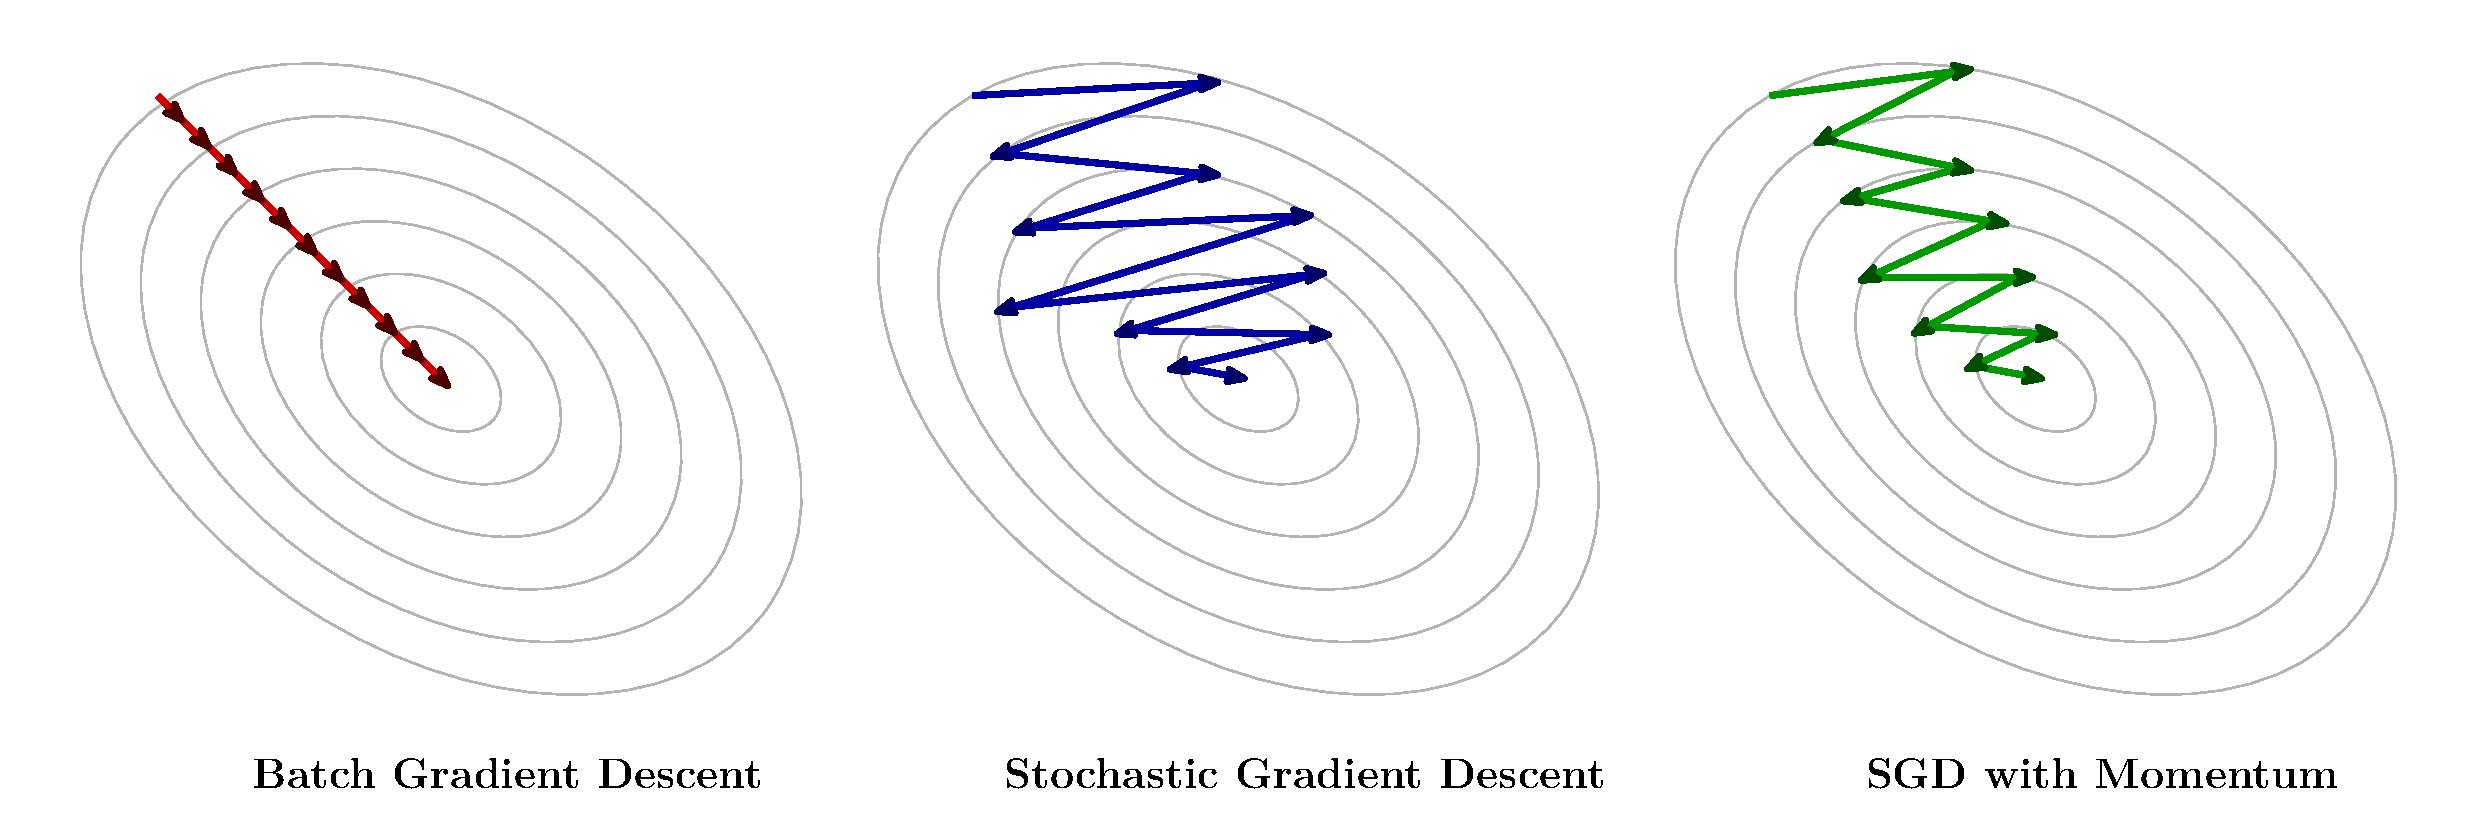
\includegraphics[width=\textwidth]{tikz/chapter3 - BGD vs SGD vs SGD with Momentum.pdf}
\caption{BGD vs SGD vs SGD with Momentum}
\end{figure}

\subsection{Stochastic Gradient Descent with Nesterov Momentum}

Stochastic Gradient Descent with Nesterov Momentum is a variant of the previous algorithm that adds a correction to the previous momentum before calculating the gradient. It works by firstly taking a step in the direction of the accumulated gradient (point 2 of the algorithm), and secondly calculating the gradient (point 4) and making the correction accordingly (point 5). (in simple momentum, we first compute the gradient and then make the correction) 

\begin{algorithm}
\renewcommand\thealgorithm{}
\caption{\textbf{\textcolor{mygreen}{Stochastic Gradient Descent with Nesterov Momentum}}}
\begin{algorithmic}[1]
\REQUIRE{Learning Rate $\varepsilon$}
\REQUIRE{Momentum Parameter $\alpha$}
\REQUIRE{Initial Parameters $\mathbf{w}$}
\REQUIRE{Initial Velocity $\mathbf{v}$}
\WHILE{Stopping Criteria not met}
\STATE Update parameters temporarily:
$\textcolor{mybluee}{\widetilde{\mathbf{w}} \leftarrow \mathbf{w} + \alpha \mathbf{v}}$
\STATE Compute gradient estimate on \textbf{\textcolor{myred}{a random training example}} $(\mathbf{x}^{(i)}, y^{(i)})$
\STATE $\mathbf{\hat{g}} \leftarrow \nabla_{\textcolor{mybluee}{\widetilde{\mathbf{w}}}} L(f(\mathbf{x}^{(i)},\textcolor{mybluee}{\widetilde{\mathbf{w}}}), y^{(i)})$
\STATE Update velocity:
$\textcolor{mybluee}{\mathbf{v} \leftarrow \alpha \mathbf{v} - \varepsilon \mathbf{\hat{g}}}$
\STATE Update parameters:
$\textcolor{mybluee}{\mathbf{w} \leftarrow \mathbf{w} + \mathbf{v}}$
\ENDWHILE
\end{algorithmic}
\end{algorithm}

The main difference between the Nesterov momentum and the standard momentum lies in \textbf{where the gradient is evaluated}. In the Nesterov momentum the gradient term is not calculated from the current position in parameter space, but rather from an intermediate position. This approach offers a significant advantage: while the gradient term always points in the optimal direction, \textbf{the momentum term may not align consistently}. Consequently, if the momentum goes in the wrong direction or overshoots the target, the gradient term can still "go back" and correct it \textbf{in the same update step}.

\newpage
\subsection{Adagrad (Adaptive Gradient Algorithm)}
The previous techniques that we have seen are based on the intuition of adjusting the learning rate while considering the history of past progress.

However, in many machine learning situations, we are faced with two distinct scenarios: a simpler one, in which all features are equally important, and a more difficult one, in which features have different levels of importance. However, up to this point, we have assigned the same learning rate to all features. \textit{Is this a valid idea?}

\begin{figure}[htbp]
\centering
\includegraphics[width=0.8\textwidth]{tikz/chapter3 - Features Importance.pdf}
\caption{Adaptive Learning Methods Intuition}
\end{figure}

Adagrad is an optimisation algorithm that \textbf{scales the model parameters by the square root of the sum of the squares of all historical gradient values}. This approach makes it possible to automatically adapt the learning rate for each parameter according to its update rate (in simple words, we take into account how much progress we have already done along each dimension and adjust the learning rate accordingly). 
\begin{algorithm}
\renewcommand\thealgorithm{}
\caption{\textbf{\textcolor{mygreen}{Adagrad}}}
\begin{algorithmic}[1]
\REQUIRE{Learning Rate $\varepsilon$}
\REQUIRE{Initial Parameters $\mathbf{w}$}
\REQUIRE{Small Constant $\delta$ to avoid division by zero}
\STATE Initialize sum of squared gradients vector: $\mathbf{r} \leftarrow 0$
\WHILE{Stopping Criteria not met}
\STATE Compute gradient estimate on \textbf{\textcolor{myred}{a random training example}} $(\mathbf{x}^{(i)}, y^{(i)})$
\STATE $\mathbf{\hat{g}} \leftarrow \nabla_{\mathbf{w}} L(f(\mathbf{x}^{(i)},\mathbf{w}), y^{(i)})$
\STATE Accumulate:
$\textcolor{mybluee}{\mathbf{r} \leftarrow \mathbf{r} + \mathbf{\hat{g}} \odot \mathbf{\hat{g}}}$
\STATE Update parameters:
$\textcolor{mybluee}{\mathbf{w} \leftarrow \mathbf{w} - \frac{\varepsilon}{\delta + \sqrt{\mathbf{r}}} \odot \mathbf{\hat{g}}}$ 
\ENDWHILE
\end{algorithmic}
\end{algorithm}

Where $\odot$ denotes element-wise multiplication.

Parameters that have large partial derivatives with respect to loss will see their learning rates reduced quickly, while those with smaller gradients will have higher learning rates, allowing for a \textbf{more stable convergence} of the model as not all direction of the optimization surface will have the same importance. 

\subsection{RMSProp (Root Mean Square Propagation)}

In many optimisation situations, Adagrad can excessively decrease the learning rate, making convergence difficult, especially in non-convex contexts. This occurs because Adagrad tends to aggressively adapt the learning rate according to the frequency of parameter updates. This means that if a parameter has a large variation in gradients during training (i.e. steep surface along that dimension), Adagrad will drastically reduce the learning rate for that parameter.

To address this problem, RMSProp has been proposed as a variant of Adagrad that \textbf{maintains an exponentially decreasing average of past gradients} (similar to momentum $\alpha v -\epsilon\hat{g}$), also called Running Average.

\begin{algorithm}
\renewcommand\thealgorithm{}
\caption{\textbf{\textcolor{mygreen}{RMSProp}}}
\begin{algorithmic}[1]
\REQUIRE{Learning Rate $\varepsilon$}
\REQUIRE{Decay Rate $\rho$}
\REQUIRE{Small constant $\delta$ to avoid division by zero}
\REQUIRE{Initial Parameters $\mathbf{w}$}
\STATE Initialize running average: $\mathbf{r} \leftarrow 0$
\WHILE{Stopping Criteria not met}
\STATE Compute gradient estimate on \textbf{\textcolor{myred}{a random training example}} $(\mathbf{x}^{(i)}, y^{(i)})$
\STATE $\mathbf{\hat{g}} \leftarrow \nabla_{\mathbf{w}} L(f(\mathbf{x}^{(i)},\mathbf{w}), y^{(i)})$
\STATE Accumulate:
$\textcolor{mybluee}{\mathbf{r} \leftarrow \rho \mathbf{r} + (1 - \rho) \mathbf{\hat{g}} \odot \mathbf{\hat{g}}}$
\STATE Update the parameters:
$\textcolor{mybluee}{\mathbf{w} \leftarrow \mathbf{w} - \frac{\varepsilon}{\delta + \sqrt{\mathbf{r}}} \odot \mathbf{\hat{g}}}$
\ENDWHILE
\end{algorithmic}
\end{algorithm}

Thanks to this strategy, RMSProp \textbf{avoids an excessive decrease in the learning rate}, as past gradients $r$ (that have been accumulated) counts less, and allows it to adapt better in non-convex contexts and to maintain a more stable convergence during optimisation. It is important to note that there is also a version of RMSProp that includes the Nesterov term, known as \textbf{RMSProp with Nesterov Momentum}, which can further improve the performance of the algorithm in certain situations.


\subsection{ADAM (ADAptive Moments)}
Adam is an optimisation algorithm that combines concepts derived from RMSProp and Momentum.  However, Adam introduces a fundamental innovation: \textbf{bias correction terms} for first and second moments. These terms and they are crucial since the first and second moments are initialised at zero and require time to "warm up" (i.e. to adapt to the data).

\begin{algorithm}
\renewcommand\thealgorithm{}
\caption{\textbf{\textcolor{mygreen}{Adam}}}
\begin{algorithmic}[1]
\REQUIRE{Learning Rate $\varepsilon$}
\REQUIRE{Decay Rates for First and Second Moments $\rho_1$, $\rho_2$}
\REQUIRE{Small constant $\delta$ to avoid division by zero}
\REQUIRE{Initial Parameters $\mathbf{w}$}
\STATE Initialize first and second moments: $\mathbf{s} \leftarrow 0$, $\mathbf{r} \leftarrow 0$
\STATE Initialize time step $t \leftarrow 0$
\WHILE{Stopping Criteria not met}
\STATE Compute gradient estimate on \textbf{\textcolor{myred}{a random training example}} $(\mathbf{x}^{(i)}, y^{(i)})$
\STATE Compute the gradient: $\mathbf{\hat{g}} \leftarrow \nabla_{\mathbf{w}} L(f(\mathbf{x}^{(i)},\mathbf{w}), y^{(i)})$
\STATE Update time step: $t \leftarrow t + 1$
\STATE Update \textbf{biased} first moment estimate:
$\mathbf{s} \leftarrow \rho_1 \mathbf{s} + (1 - \rho_1) \mathbf{\hat{g}}$ \qquad \quad \qquad \COMMENT{\textbf{\textcolor{gray!90!white}{Momentum Idea}}}
\STATE Update \textbf{biased} second moment estimate:
$\mathbf{r} \leftarrow \rho_2 \mathbf{r} + (1 - \rho_2) \mathbf{\hat{g}} \odot \mathbf{\hat{g}}$ \qquad \COMMENT{\textbf{\textcolor{gray!90!white}{RMSProp Idea}}}
\STATE Correct bias in first moment: $\textcolor{mybluee}{\hat{\mathbf{s}} \leftarrow \frac{\mathbf{s}}{1 - \rho_1^t}}$
\STATE Correct bias in second moment: $\textcolor{mybluee}{\hat{\mathbf{r}} \leftarrow \frac{\mathbf{r}}{1 - \rho_2^t}}$
\STATE Update parameters:
$\textcolor{mybluee}{\mathbf{w} \leftarrow \mathbf{w} - \varepsilon \frac{\hat{\mathbf{s}}}{\delta + \sqrt{\hat{\mathbf{r}}}}}$
\ENDWHILE
\end{algorithmic}
\end{algorithm}

Adam automatically adapts the learning rates for each parameter based on momentum and past momentum estimation, helping to improve the effectiveness of optimisation during the learning process. In Adam, we combine several concepts seen in this section: the \textbf{use of the stochastic} in the SGD, the \textbf{idea of using momentum}, the \textbf{adaptation of the learning rate based on the second moment} and the \textbf{use of a bias correction} for both moments.


\section{Normalization}

\vspace{-0.4cm}
In the world of neural networks, optimization is crucial to model success. However, simply adopting SGD may not be enough. Deep neural networks are known to be difficult to train, for example, one of the main problems we face during optimization is the so-called "Covariate Shift."
\vspace{-0.4cm}

\subsection{The Problem of Covariate Shift}

When training a neural network, it is important to keep the distribution of input data stable throughout the training process. If the distribution changes significantly during training, the model may have difficulty generalising well to new data, as patterns learned during training may no longer be relevant or representative.

The main problem arising from the covariate shift is that it can lead to a situation where \textbf{most of the input data falls into non-linear regions} of the neural network's activation function. This can significantly \textbf{slow down the learning process} as the network may require multiple iterations to adapt its weights effectively to the new input distributions.

To address the Covariate Shift problem and improve the training of neural networks, a fundamental concept was introduced: \textbf{Batch Normalization}.

\subsection{Batch Normalization}

It is a method for reconfiguring the parameters of a deep network, which \textbf{can be applied to the input layer as well as to any hidden layer}.

The key concept behind Batch Normalization is the standardization of the inputs of a network layer. This is done by subtracting the mean of the inputs and dividing by the standard deviation. In mathematical terms, if $ \mathbf{H} $ represents the outputs of a layer, $ \mu $ and $ \sigma $ represent the mean and standard deviation (both vectors) calculated on the columns (features) of $ \mathbf{H} $, then the transformation is given by:
$$ \mathbf{H}' = \frac{\mathbf{H} - \mu}{\sigma} $$ where $$\mu = \frac{1}{m}\sum_{}^{j}\mathbf{H}_{:,j}$$
$$\sigma = \sqrt{\delta + \frac{1}{m}\sum_{j}^{}(\mathbf{H}-\mu)^2_j}$$
\textit{The term $\delta$ in the formula represents the usual small constant added to avoid numerical problems when the calculated standard deviation is very close to zero. }
Standardizing the output of a unit could limit the expressive power of the neural network because, without introducing additional parameters, normalization could bring all features in a given stratum to a common scale, making it more difficult for the neural network to capture complexity and variation in the data. This is because standardization unifies features, bringing them to \textbf{a mean of zero and a standard deviation of one}, potentially "squeezing" them into a narrower range.

To mitigate this problem and allow the neural network to maintain its expressive capability, two additional parameters are introduced in Batch Normalization: the \textbf{scaling factor} ($ \gamma $) and the \textbf{bias} ($ \beta $). These parameters allow the network to learn a linear transformation of the normalized output, thus allowing greater flexibility in data representation. 
$$\text{Output} = \gamma \mathbf{H}' + \beta $$
Essentially, the scaling factor and bias allow the network to adapt to a wide range of data while maintaining its ability to express and learn complex patterns as they are learned during the back-propagation process.

During training, back-propagation is performed through normalized activations and these two parameters ($\gamma$ and $\beta$) are also learned. During testing, on the other hand, running averages of $ \mu $ and $ \sigma $ collected during training are used to evaluate new entries.

% Batch Normalization offers several advantages, including improving gradient flow, enabling the use of higher learning rates, reducing dependence on initial parameters, and functioning as a form of regularization to improve stability and prevent overfitting during neural network training.

\subsection{Batch, Layer or Instance Normalization?}

There are two famous variants of Batch Normalization: \textbf{Layer Normalization} and \textbf{Instance Normalization}. Briefly summarised, the difference is that Batch Normalization normalises across the entire batch, Layer Normalization normalises across the entire layer and Instance Normalization normalises each instance individually. \textit{I know, it's not very intuitive, so let's do a more detailed analysis!}

To explain the various concepts, we will use a tuple \textbf{(N,C,H,W)}, which is commonly used to represent multidimensional data such as images (\textit{which will be the focus of our example to give us a better understanding}). This representation is nothing more than a tensor and is common in frameworks such as TensorFlow and PyTorch to handle input data in neural networks. Here is what each dimension represents:
\begin{itemize}
    \item \textbf{N}: Represents the \textbf{batch size}, i.e. the number of instances (or samples) within the batch. For example, if N=32, this means we are working with a batch of 32 images.
    \item \textbf{C}: Indicates the \textbf{number of channels} (feature maps) in the data. In a colour image, we will typically have 3 channels for the colours red, green and blue (RGB). In general, in the input data, the channel can represent not only the colour, but various aspects or features of the input, such as depth, features extracted from convolutional layers, etc.
    \item \textbf{H}: Represents the \textbf{height of the data}. In an image, it corresponds to the number of rows of pixels present.
    \item \textbf{W}: Represents the \textbf{width of the data}. In an image, it corresponds to the number of columns of pixels present.
\end{itemize}
H and W will be merged together (\textit{Sorry, but my drawing skills stop at 3 dimensions \faSadTear[regular]}).
We will also use a small example: let us consider a batch with 10 images, each of which has 3 features (RGB) and the image size is 100x100. Let's start then:


\begin{minipage}{0.4\textwidth}
\textbf{\textcolor{mybluee!70}{Batch Normalization (BN):}} \\

Consider the entire batch of size N. Each example in the batch has C channels, each of which has an image of size HxW. With Batch Normalization, we normalise the data on each channel across the entire batch. Then, for each channel, we calculate the mean and standard deviation over all examples in the batch and normalise the data on that channel accordingly.
\end{minipage}
\begin{minipage}{0.05\textwidth}
\ 
\end{minipage}
\begin{minipage}{0.55\textwidth}
\includegraphics[width=\textwidth]{tikz/chapter3 - Batch Norm.pdf}
\captionof{figure}{Batch Norm Multidimensional Data}
\end{minipage}

Taking our example, we would have a tensor of size (10, 3, 100), where:
10 represents the batch size (N), i.e. the number of images in the batch,
3 represents the number of channels (C), such as the three colour channels: red, green and blue,
100 represents the height (H) of the image and
100 represents the width (W) of the image.
For each colour channel in each image, the mean and standard deviation on all pixels corresponding to that colour channel in all images in the batch would be calculated. The pixel values for each colour channel \textbf{in each image} would then be normalised against these calculated mean and standard deviations.



\begin{minipage}{0.55\textwidth}
\includegraphics[width=\textwidth]{tikz/chapter3 - Layer Norm.pdf}
\captionof{figure}{Layer Norm Multidimensional Data}
\end{minipage}
\begin{minipage}{0.05\textwidth}
\ 
\end{minipage}
\begin{minipage}{0.4\textwidth}
\textbf{\textcolor{myred!70}{Layer Normalization (LN):}} \\

Here, we consider each example in the batch separately. Each example has C channels (features!), each of which has an image of size HxW. With Layer Normalization, we normalise the data of each channel for each example. Then, for each channel, we calculate the mean and standard deviation over the entire input of that example (i.e. over all positions of HxW) and normalise the data of that channel accordingly.
\end{minipage}

Once again, we would have a tensor of size (10, 3, 100).
However, each image in the batch is considered separately. For each image, the pixel values in each colour channel would be normalised with respect to the distribution of pixel values within the same image.
Thus, the pixel values in each image would be normalised to the distribution of pixel values within the image itself, \textbf{completely ignoring the other images in the batch}.


\begin{minipage}{0.4\textwidth}
\textbf{\textcolor{mygreen!70}{Instance Normalization (IN):}} \\

We consider each spatial position (HxW) separately for each example in the batch. Each position has C channels. With Instance Normalization, we normalise the data of each channel for each position in the image. Then, for each channel, we calculate the mean and standard deviation over all positions in the image for each example in the batch and normalise the data for that channel accordingly.
\end{minipage}
\begin{minipage}{0.05\textwidth}
\ 
\end{minipage}
\begin{minipage}{0.55\textwidth}
\includegraphics[width=\textwidth]{tikz/chapter3 - Instance Norm.pdf}
\captionof{figure}{Instance Norm Multidimensional Data}
\end{minipage}

Here again, we have the same size tensor (10, 3, 100).
Now, each pixel in each colour channel of each spatial position in the image is considered separately for each image in the batch.
The pixel values at each spatial position (HxW) of \textbf{each colour channel in each image} would be normalised to the corresponding pixel values at the same positions in the other images in the batch.

\textbf{N.B.} A more modern technique is \textbf{Group Normalisation (GN)}, which can be considered as a mix between Layer Normalisation and Instance Normalisation. With GN, the data channels are considered separately, as in Layer Normalisation, but instead of operating on an entire layer, the \textbf{channels are divided into groups} and the normalisation statistics within each group are calculated independently. This approach is reminiscent of the idea of instance-based normalisation, where each instance is considered separately, but instead of normalising individual instances, GN normalises groups of channels. This makes it useful in scenarios where the dimensionality of the data is high and normalisation on entire layers may be excessive.


\newpage
\chapter{Regularization}
\setbackgroundchapter{Regularization}
\section{Model Capacity and Overfitting}

The capability of a model refers to its \textbf{ability to fit a wide range of functions}. Indeed, it represents the intrinsic complexity of the model and its ability to capture relations in the data. \textit{In other words, it describes how complex is the function it represents.}

Models with low capacity may have difficulty adapting to the training set, while those with high capacity may suffer from overfitting, that is, overfitting to the training data leading to poor generalization to new data.

Model capacity is closely related to the hypothesis space, which represents the set of all features that the model can potentially learn. A model with a higher capacity will have access to a larger hypothesis space, allowing it to learn more complicated relationships in the data.

\begin{figure}[!htbp]
    \centering
    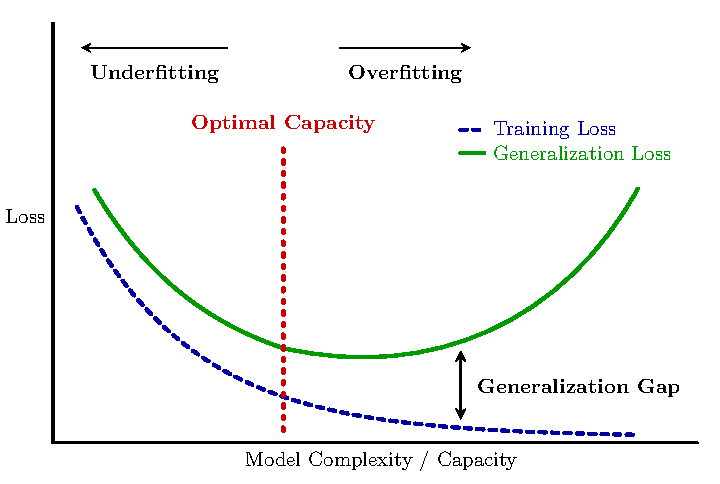
\includegraphics[width = \linewidth]{tikz/chapter4 - Model Capacity.pdf}
    \caption{Complexity of a Model with respect to the Losses}
\end{figure}

In the figure above, it is evident that as the complexity of the model increases, the loss on the training set tends to decrease, while the loss on generalization (e.g., on the test set) may increase, causing a gap between the losses known as the \textbf{generalization gap}.

To deal with overfitting, it is important to choose a model with the right capacity. This means setting the capacity so that it is high enough to capture the main regularities in the training data, but not so high that it also captures spurious regularities or noise in the data. \textit{Basically, it is a matter of finding a balance between the complexity of the model and its capacity for generalization.}

In addition to controlling model capacity, there are other strategies to reduce overfitting. For example, \textbf{collecting more training data} can help the model better capture the variety of relationships in the data. Alternatively, \textbf{ensembling techniques}, such as averaging many different models (e.g. bagging), can be used. These strategies help avoid overfitting to training data, allowing the model to generalize better to new data.

\textit{Are there alternatives to cope with overfitting? Yes, regularization techniques! These provide effective tools for optimizing model performance. In the next sections, we will dive into the details of these powerful assets!}

To give you a taste, here is an overview of the various regularization strategies we will see:

\begin{figure}[!htbp]
    \centering
    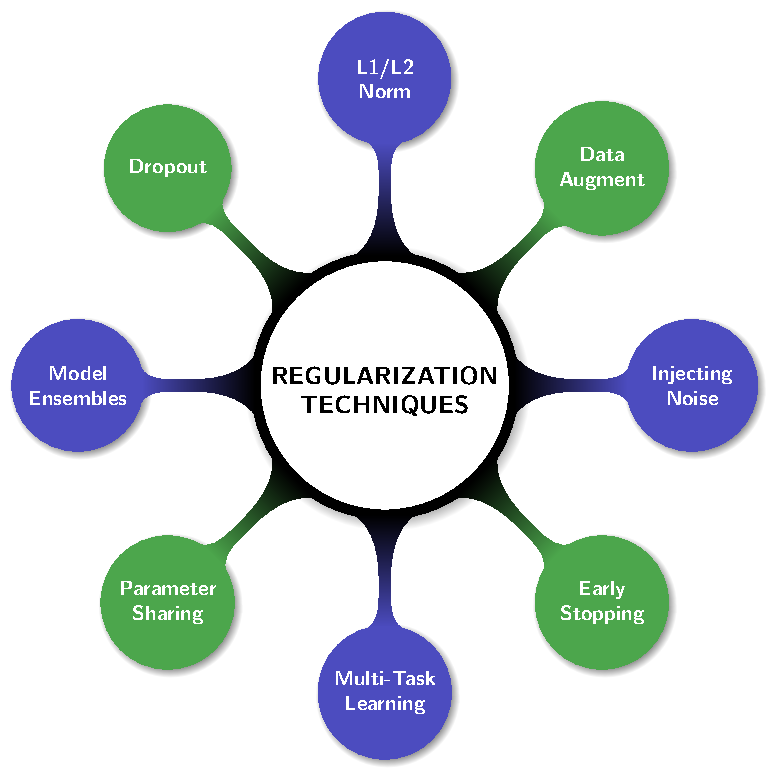
\includegraphics[width = 0.8\linewidth]{tikz/chapter4 - Regularization Schema.pdf}
    \caption{Different Regularization Strategies}
\end{figure}

\section{Parameter Norm Penalties}

We start with this first type of normalization in which we add a penalty to the loss function during training, which then \textbf{affects the size of the weights (parameters)} of the model. Here is the general formula for the error function:

$$
\tilde{L}(\mathbf{W}) = L(\mathbf{W}) + \lambda \Omega(\mathbf{W})
$$

The \textbf{\textcolor{myred}{Regularization L2}}, also known as \textbf{\textcolor{myred}{Ridge}}, adds a term to the loss function proportional to the \textbf{\textcolor{myred}{square norm of model weights}}. Mathematically, the formula for L2 regularization is given by:

$$
\Omega(\mathbf{W}) = \frac{1}{2} \sum_{l} ||\mathbf{w}_l||^2
$$

This is inserted into the error function, obtaining the regularized loss function $\tilde{L}(\mathbf{w})$:

$$
\tilde{L}(\mathbf{W}) = \sum_{i=1}^{n} L(f(x_i, \mathbf{W}), y_i) + \textcolor{myred}{\frac{\lambda}{2} \sum_{l} ||\mathbf{w}_l||^2}
$$

Where:
\begin{itemize}
    \item $\sum_{i=1}^{n} L(f(x_i, \mathbf{W}), y_i)$ represents the sum of losses on all training data $(x_i, y_i)$.
    \item $\frac{\lambda}{2} \sum_{l} ||\mathbf{w}_l||^2$ represents the L2 regularization term, where $|\mathbf{w}_l||^2$ is the squared norm of the model weights and $\lambda$ is the regularization parameter.
    \item The sum over $l$ represents the sum over all the weights of the model.
\end{itemize}

$\lambda$ is \textbf{the hyperparameter that controls the importance of regularization}, i.e., it determines how much weight to give to the penalty of the model weights with respect to performance on the training data.

The use of L2 regularization leads the model weights to \textbf{tend to smaller values}, thus avoiding extremely high values that could lead to overfitting. In addition, this technique promotes the creation of simpler models.

On the other hand, the \textbf{\textcolor{mygreen!90!black}{Regularization L1}}, also known as the \textbf{\textcolor{mygreen!90!black}{Lasso}}, adds a term to the loss function proportional to the \textbf{\textcolor{mygreen!90!black}{absolute norm of model weights}}. The L1 regularization formula is expressed as:

$$
\Omega(\mathbf{W}) = \sum_{l} |\mathbf{w}_l|
$$

Again, we insert in the loss function:

$$
\tilde{L}(\mathbf{W}) = \sum_{i=1}^{n} L(f(x_i, \mathbf{W}), y_i) + \textcolor{mygreen!90!black}{\lambda \sum_{l} |\mathbf{w}_l|}
$$

Where:
\begin{itemize}
    \item $\sum_{i=1}^{n} L(f(x_i, \mathbf{W}), y_i)$ represents the sum of losses on all training data $(x_i, y_i)$.
    \item $\lambda \sum_{l} |\mathbf{w}_l|$ represents the L1 regularization term, where $||\mathbf{w}_l|$ is the absolute norm of the model weights and $\lambda$ is the regularization parameter.
    \item The sum over $l$ represents the sum over all the weights of the model.
\end{itemize}

Unlike L2 regularization, L1 regularization favors \textbf{sparsity of weights}, that is, many weights tend to become exactly zero. This behavior is also useful for feature selection, since it makes the features most relevant to the model more obvious.

To summarize, here is a figure that visually shows how L1 and L2 regularization affect model weights differently:

\begin{figure}[!htbp]
    \centering
    \includegraphics[width = \linewidth]{tikz/chapter4 - L1 and L2 plot.pdf}
    \caption{L1 Regularization and L2 Regularization Plots}
\end{figure}


The plot represents the space of model weights/parameters.

In the center of the gradient error is the point where the model error is lowest. At this point, the model shows the best performance on the training data.

Next, you will notice an overlap between the gradient error and the gradient of the L1 or L2 norm penalty. This is an optimization point where the overall model error is minimized, also taking into account the regularization penalty. Here the \textbf{right balance between error reduction and model complexity} is achieved, thus avoiding both underfitting and overfitting.

For \textbf{\textcolor{mygreen}{L1 regularization}}, it will be observed that many of the weights in the model will touch the L1 Norm function in the zero abscissa, representing null weights. This indicates that L1 regularization \textbf{favors sparsity of the weights}.

For \textbf{\textcolor{myred}{L2 regularization}}, you will notice a gradual reduction of the weights, but none will be exactly zero. This represents that L2 regularization acts more uniformly, \textbf{reducing the magnitude of the weights without completely zeroing them}.

\section{Data Augmentation}

One of the main challenges in training models is the availability of sufficient and diverse training data. Data augmentation is a strategy that aims to improve model generalization by \textbf{increasing the amount and variety of training data}. The idea behind it is that the more training data we have, the better the model can learn to generalize to new data not seen during training.

Data augmentation is particularly effective in classification tasks, where it is relatively easy to generate new samples by transforming existing ones. This approach is based on the fact that the \textbf{main task of the classifier is to be invariant to a wide range of transformations of the input data}. For example, in the case of images, we can generate new samples by applying transformations such as rotation, translation, color change, scaling, and so on. The goal is to create a diversity of samples that cover as much of the input data space as possible, thus helping the model learn a more robust and general representation of discriminative features.
    
Some problems may require special precautions during data augmentation. For example, in the context of character recognition using datasets such as MNIST, it is important not to apply transformations that would change the class, such as transformations that might turn a '6' into a '9'.
    
Data augmentation can also be applied to different types of data, such as \textbf{acoustic and textual data}. For example, for acoustic data, transformations such as pitch shift, stretching time and dynamic range compression can be applied. For textual data, one can use techniques such as substitution, deletion, and letter insertion, or use synonyms and modify adjectives.

\section{Injecting Noise}

Gaussian noise as input can be used as a regularizer in neural models. Specifically, each component of the input \( x_i \) can be modified by adding Gaussian noise \( \mathcal{N}(0, \sigma_i^2) \), so the equation becomes:

$$ x_i = x_i + \textcolor{mybluee}{\mathcal{N}(0, \sigma_i^2)} $$

As for the output \( y_j \) of a layer, it can be expressed as the sum of the original output and the Gaussian noise \textbf{amplified by the weight squared}, so the equation becomes:

$$ y_j = y_j + \textcolor{mybluee}{\mathcal{N}(0, w_i^2 \sigma_i^2)} $$

where \( N(0, \sigma_i^2) \) represents Gaussian noise with zero mean and variance \( \sigma_i^2 \), \( w_i \) represents the weight associated with the input \( x_i \).

This contributes additively to the quadratic error, causing the model to minimize the overall error, which then \textbf{tends to minimize the square weights as well}. This effect is similar to L2 regularization through noisy inputs. 

\textbf{High levels of noise generate a smoother function}. This is useful in applications where a smooth function is preferred.

In \textbf{autoencoder models for denoising}, noise injection is a common practice. The goal is to teach the neural network to reconstruct the original input from the noisy input. This technique is often used in unsupervised learning algorithms.

\textit{But can noise only be added to inputs? Absolutely not! It can also be added to weights and labels in neural models!} Adding noise to the inputs makes the learned function smoother, while \textbf{adding noise to the weights encourages the network to be more robust to random variations in the training data} (we get a kind of "flexibility" in the model's weights). This can be especially useful when the model is in regions of the weight space where variations in individual weights do not significantly affect the model output. \textbf{Adding noise to labels can discourage overconfident model behavior}, such as during cross-entropy loss learning, thus preventing overestimation of class probabilities (cross-entropy assigns very large values for the for the correct class and very small values for the wrong classes). A common practice in this case is the application of "\textbf{label smoothing}", which is the random modification of labels.

\section{Early Stopping}

Early Stopping is a technique used in model training to prevent the model from becoming too specialized on the training data. 
This technique is based on the idea of monitoring the performance of the model on a validation dataset during training and \textbf{stopping training when the performance on the validation set starts to deteriorate, even if the performance on the training set continues to improve}.

The number of training steps is seen as another \textbf{hyperparameter that needs to be optimized}. The Early Stopping procedure can be summarized in the following steps: It starts with small initial weights. Each time the error on the validation set improves, you keep a copy of the model parameters. When training ends, you return the parameters \textbf{for which the validation error is smallest}.

However, it is \textbf{important to select the stopping point correctly}, since an early stopping point could prevent the model from learning important information, while stopping too late could lead to overfitting. Consequently, the number of epochs or iterations before stopping must be carefully selected during the training phase.

\section{Multi-Task Learning}

Multi-Task Learning is a learning technique where the model is trained to do \textbf{more than one task at the same time}. For example, we might want to train a model to recognize objects in an image and simultaneously identify their location. This means that the model learns to perform more than one "task" during the same training process.

In Multi-Task Learning, several tasks \textbf{share the same set of input data and some intermediate layers of the neural network}, but may have \textbf{separate final layers for each task}. In this case, the parameters can be of two types: \textbf{task-specific} or \textbf{generic} (shared among all tasks). The former are designed to perform a specific task and learn only from data related to that task (typically found in the upper layers of the network), while the latter are shared across all tasks and can benefit from the combined data of all tasks (typically found in the lower layer of the network).

Multi-Task Learning often compares with self-supervised learning. While in Multi-Task Learning multiple tasks are taught at the same time, \textbf{in self-supervised learning the model learns to represent data in such a way that some information is "hidden"} and must be predicted. For example, it might train a model to predict missing parts of a picture.

In Multi-Task Learning, it is possible to apply \textbf{soft constraints on model parameters}. This means that we can enforce some parameters to be similar to others (this is called \textbf{"Paramaters Tying"}). For example, if we have multiple models performing the same type of classification but with slightly different data, we can force the parameters to be similar to ensure consistency across models.

\section{Parameters Sharing}
\label{c4:parameterSharing}
Parameter Sharing is a technique used in neural networks to enforce that \textbf{certain parameters within the network are exactly the same}. This is done for several reasons, including reducing model complexity and sharing relevant information between different parts of the network.

Sharing parameters within the network offers an advantage over "Paramaters Tying", since only a subset of the parameters need to be stored in memory.

In convolutional neural networks (CNNs), used primarily in computer vision, parameter sharing is a key feature. This is based on two main properties of CNNs:

\begin{itemize}
    \item \textbf{Local Connectivity}: Neurons in one layer are \textbf{connected to only a small region of the previous layer}. This feature allows CNNs to capture local image features.
    \item \textbf{Weight Sharing between Spatial Positions}: This feature allows CNNs to learn displacement-invariant filter kernels, reducing the number of parameters needed and ensuring that the model is \textbf{able to recognize the same features in different parts of the image}. For example, a picture of a cat remains a picture of a cat even if it is shifted by some pixel. 
\end{itemize}

\section{Model Ensembles}

In this technique, instead of relying on a single model, we train several models separately and then have all the models vote on the output for the test examples. The idea behind it is that \textbf{different models will usually make different errors on the test set}. Therefore, by combining the predictions of multiple models, a better overall result can be obtained. \textit{This technique is similar to consulting multiple experts to get more reliable advice.}

One of the most common methods of implementing Model Ensembles is \textbf{Bagging} (Bootstrap Aggregating). In Bagging, several instances of the same model type are trained on \textbf{random subsets of the training set (with replacement)} and then the \textbf{predictions of all models are combined}. 

However, this method requires more computational resources and can be more complex to implement and manage than a single model.

\section{Dropout}

The basic idea of Dropout is to \textbf{randomly turn off some neurons} during the forward pass (forward pass) of the network. This process is \textbf{stochastic}, since the choice of neurons to be eliminated is random. By forcing the network to work with redundant representations, Dropout prevents hidden neurons from fitting too closely to each other and \textbf{forces them to focus on extracting more useful features} for the task.

Dropout can be viewed as training a large set of models, each of which shares network parameters. Each binary Dropout mask leads to a different model, and for each example, the network is trained using a different Dropout mask. \textit{Each value in the mask represents whether the corresponding neuron is active (1) or deactivated (0) during the forward pass of the network.}

Dropout is similar to Bagging, but is more practical. Whereas in Bagging one defines \( k \) different models and builds \( k \) different datasets by sampling from the dataset with replacement, \textbf{Dropout aims to approximate this process with exponentially large numbers of neural networks}.

\begin{figure}[!htbp]
    \centering
    \includegraphics[width = \linewidth]{tikz/chapter4 - Dropout.pdf}
    \caption{Visualization of the Dropout Technique}
\end{figure}

During training, at each step, a binary Dropout mask with a certain inclusion probability is randomly extracted for each neuron. This mask is then used to deactivate some neurons during the forward transition of the network. During testing, ideally we would like to integrate all probability contributions for all masks, but this is \textbf{computationally expensive}. Therefore, we use a \textbf{Monte Carlo approximation}, performing many forward steps with different Dropout masks and averaging all predictions. It has been shown that this procedure is equivalent to taking the average of all possible neural networks.



\newpage
\chapter{Convolutional Neural Networks}
\setbackgroundchapter{Convolutional Neural Networks}
Welcome to the second part of the course, in which we delve into the intricate world of \textbf{different neural network architectures}. \textit{If things seemed complicated before, they will get even more challenging here.} \emoji{smiling-face-with-tear}

Convolutional Neural Networks (CNN) handles \textbf{structured data}, such as images. Various architectures have been developed, each attempting different methods to learn effective representations of structured data. In the case of images, these representations capture \textbf{spatially local dependencies} between pixels. The low-level layers of a CNN extract local features, while the high-level layers extract learn global
patterns.

\textit{To understand Convolutional Neural Networks, think of our brain. When we look at an image, the brain processes it in different parts. At first, it recognises simple things like lines and angles. Then, it moves on to more complicated things, until it understands the complete object.}

\textit{The cells in the brain are like small parts that only look at one part of the image. This helps to focus only on the important things. There are two main types of these cells: some look at small and close things, others look at larger things and care less about the exact position.}

\begin{figure}[!htbp]
    \centering
    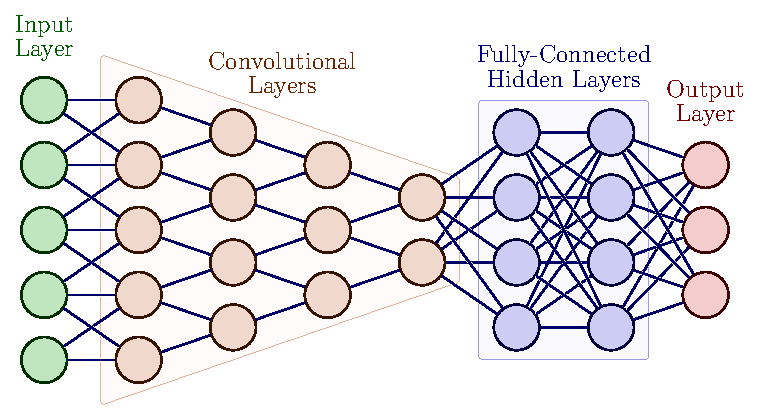
\includegraphics[width=\textwidth]{tikz/chapter5 - CNN.pdf}
    \caption{Example of a Convolutional Neural Network}
\end{figure}

Convolutional Neural Networks represent a \textbf{specialised version of feedforward neural networks}. If we were to apply a feedforward neural network to process an image, we would lose important information on the spatial relationships between pixels and would have to deal with a large number of parameters due to the need to treat the image as a long input vector. This situation therefore necessitates a complete redesign of the architecture.

CNNs are designed with some specific features, discussed in the previous chapter, that define their recurrent module. These features include \textbf{local connectivity} and \textbf{weight sharing}, which allow these architectures to effectively capture the spatial characteristics of images without having to manage an excessive number of parameters.

\section{Convolutions}

Convolutional Neural Networks basically \textbf{replace general matrix multiplication with convolution in at least one of their layers}. A convolution is an operation that takes a matrix (a portion of an image corresponding to the size of the so-called kernel) as input and produces a scalar by calculating the scalar product between the pixel values of the area and the kernel parameters. By progressively moving the kernel, the final output of the convolutional layer will be a matrix. 

Formally, a Convolutional Layer consists of a set of filters, each covering a small spatial portion of the input, known as the \textbf{receptive field}. Each filter is convoluted along the dimensions of the input data, producing a multidimensional feature map representing the filter's responses to various fragments of the input data. \textbf{During training, the network learns filters that are activated in response to specific features at specific spatial locations}.

This concept can be formalised as follows:
$$
S(i,j) = \sum_{m}\sum_{n} I(m,n)K(i-m,j-n)
$$
Convolutional layers help to extract local features from an image using filters, which are learnt during training as they store weights. However, in a CNN, \textbf{filters} are not learnt randomly; rather, they \textbf{are optimised to best fit the architecture, loss function and data}.


\begin{figure}[!htbp]
    \centering
    \includegraphics[width=\textwidth]{tikz/chapter5 - Convolution.pdf}
    \caption{Example of a 2D Convolution}
\end{figure}
An example of convolution is shown in the figure above, in which we have this kernel and calculations:

\hspace{0.05\textwidth}
\begin{minipage}{0.4\textwidth}
$$
\begin{pmatrix}
\mathbf{\textcolor{mygreen}{1}} & \mathbf{\textcolor{mygreen}{0}} & \mathbf{\textcolor{mygreen}{1}} \\[-0.2cm]
\mathbf{\textcolor{mygreen}{0}} & \mathbf{\textcolor{mygreen}{1}} & \mathbf{\textcolor{mygreen}{0}} \\[-0.2cm]
\mathbf{\textcolor{mygreen}{1}} & \mathbf{\textcolor{mygreen}{0}} & \mathbf{\textcolor{mygreen}{1}} \\
\end{pmatrix}
$$
\end{minipage}
% \hspace{0.05\textwidth}
\begin{minipage}{0.4\textwidth}
$$
\begin{aligned}
&\mathbf{\textcolor{myred}{1}} \times \mathbf{\textcolor{mygreen}{1}} + \mathbf{\textcolor{myred}{0}} \times \mathbf{\textcolor{mygreen}{0}} + \mathbf{\textcolor{myred}{0}} \times \mathbf{\textcolor{mygreen}{1}}&\\
+ &\mathbf{\textcolor{myred}{1}} \times \mathbf{\textcolor{mygreen}{0}} + \mathbf{\textcolor{myred}{1}} \times \mathbf{\textcolor{mygreen}{1}} + \mathbf{\textcolor{myred}{0}} \times \mathbf{\textcolor{mygreen}{0}}&\\
+ &\mathbf{\textcolor{myred}{1}} \times \mathbf{\textcolor{mygreen}{1}} + \mathbf{\textcolor{myred}{0}} \times \mathbf{\textcolor{mygreen}{0}} + \mathbf{\textcolor{myred}{1}} \times \mathbf{\textcolor{mygreen}{1}}&=\mathbf{\textcolor{mybluee}{4}}\\
\end{aligned}
$$
\end{minipage}
\hspace{0.05\textwidth}

For the input considered, the convolution is calculated through the scalar product between the kernel values and the corresponding input values. 
The result of this calculation is 4, which represents the output of this specific convolution.

It is important to know two fundamental parameters used to control the size of the convolution output and influence the size and shape of the features extracted by the convolutional neural network, namely:
\begin{itemize}
    \item \textbf{Padding}: Padding refers to the addition of values (commonly zeros) around the edges of the input image before applying the convolution. This is useful for controlling the size of the convolution output. Padding may be "\textbf{Valid}" (no padding) or "\textbf{Same}" (padding so that the output is the same size as the input, also called \textbf{zero-padding}).
    \item \textbf{Stride}: The stride indicates the number of pixels in which the filter (kernel) is moved along the input image during the convolution operation. \textbf{A stride value greater than one} results in a larger displacement, reducing the size of the output. \textbf{A stride value of one} is the most common and produces an output with the same size as the input.
\end{itemize}

\begin{figure}[!htbp]
    \centering
    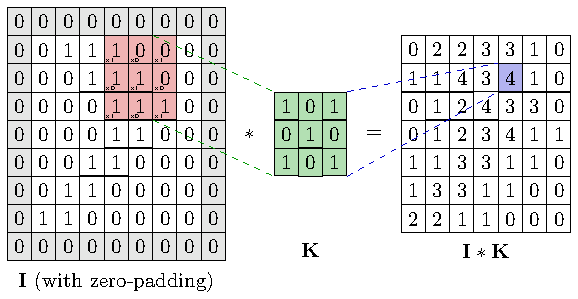
\includegraphics[width=\textwidth]{tikz/chapter5 - Convolution with Padding.pdf}
    \caption{Example of a 2D Convolution with Zero-Padding}
\end{figure}

The output of the convolutional layer depends on the size of the kernel $K$, the stride $S$, the padding $P$, and can be calculated using the formula $\mathbf{\frac{(N-K)+2P}{S}+1}$, where $N$ is the size of the input. In the case of our example, the input is a square matrix of size 7x7, the kernel is 3x3, the padding is 1 and the stride is 1, so the output will be a matrix of size 5x5.

\textbf{N.B.} It is important to note that when we speaks of "two-dimensional convolutions", we are actually working with three-dimensional tensors (volumes). Thus, the example of the two-dimensional convolution given above does not fully reflect the complexity of convolutions in CNNs. In fact, when exploring various architectures, such as AlexNet or VGGNet, it is evident that the drawings of the various layers show the use of three-dimensional tensors. If you want to try and explore this further, here is a useful link that shows what these convolutions actually look like visually: \underline{\href{https://animatedai.github.io/}{Animated AI Convolution}}.


\section{Inside a CNN}

Here's an overview of what happens inside a Convolutional Neural Network:  
\begin{remark}{accent}{accent!5}
\textbf{Input image}: This layer represents the raw image entering the network. Generally, images are represented as multidimensional arrays of pixels, where each pixel has a value indicating its light intensity or color.
\end{remark}

\begin{remark}{mybluee}{mybluee!20}
\textbf{Convolution layer}: This is where the convolution operation takes place, which is fundamental for extracting features from the input image. Here, filters (or kernels) are applied to the image to detect specific patterns. \textbf{Each filter}, as it flows over the entire image, \textbf{produces a feature map}, highlighting the presence of edges, shapes and textures. \textit{It is as if each small region of the image participates in a "discussion" process to identify its unique features, and the different filters carry on this discussion, each highlighting different aspects.} The size of a filter is not constrained, allowing the network to adapt and learn different aspects of the images.
\end{remark}


\begin{remark}{myred}{myred!20}
\textbf{Non-linearity}: After convolution, a non-linear activation function such as ReLU is applied. This layer adds non-linearity to the model, allowing the network to learn and represent complex relationships between image features, without affecting the
receptive fields. 
\end{remark}

\begin{remark}{mygreen}{mygreen!20}
\textbf{Spatial Pooling}: This layer reduces the size of feature maps obtained by convolution, reducing the number of parameters and controlling overfitting. Commonly used are \textbf{max pooling} or \textbf{average pooling} layers, which reduce the size of the feature map by \textbf{preserving only the most significant values}. This also helps to create a \textbf{spatially invariant representation}, as relevant features are preserved even if slightly shifted in the image. \textit{So, the network is able to classify a photo of a dog even if it is translated in the image.}
\end{remark}

\begin{remark}{myorange}{myorange!20}
\textbf{Normalization Layer}: This layer is optional and can be used to normalise feature maps before passing them on to the next layer of the network. As we have seen, Normalization can be useful to ensure that \textbf{data remain in an appropriate range} and to facilitate the network learning process.
\end{remark}

\begin{remark}{accent}{accent!5}
\textbf{Feature Maps}: The feature maps resulting from the previous steps represent the information extracted from the input image. Each feature map corresponds to a specific feature detected by the network and can be interpreted as a \textbf{simplified representation of the image in terms of relevant patterns and structures}. These feature maps are then used as input to subsequent layers of the network for further processing and analysis.
\end{remark}
\textit{Nope, the colors are not related with the colors in the pictures above, sorry.}

\section{CNN Architectures (for Classification)}

Let's now discover the main architectures of Convolutional Neural Networks, from the pioneer LeNet to the modern ConvNeXt, which have revolutionised image recognition!

\subsection{LeNet (1998)}
LeNet was the \textbf{milestone that initiated the field of Convolutional Neural Networks}, developed at AT\&T Labs. Its impact has been instrumental in promoting the use of Convolutional Neural Networks in character recognition and other computer vision applications. Its main features include:
\begin{itemize}
    \item Uses \textbf{convolutional and subsampling} (pooling) followed by fully connected layers.
    \item \textbf{Requires complete retraining when image resolution changes}.
    \item Article: \href{http://vision.stanford.edu/cs598_spring07/papers/Lecun98.pdf}{"Gradient-Based Learning Applied to Document Recognition" (LeCun et al.)}
\end{itemize}

\begin{figure}[!htbp]
    \centering
    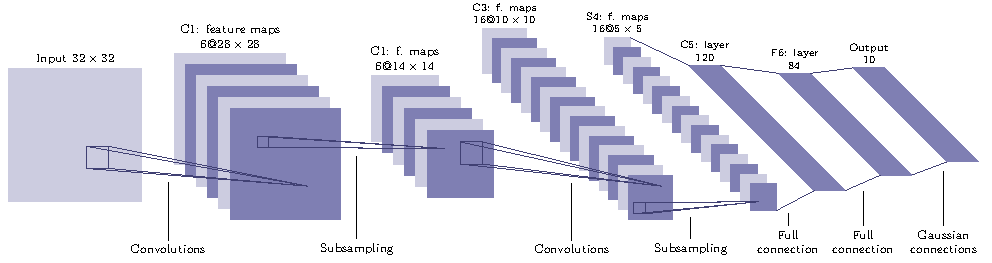
\includegraphics[width=\textwidth]{tikz/chapter5 - LeNet.pdf}
    \caption{LeNet Architecture}
\end{figure}

\subsection{AlexNet (2012)}
AlexNet marked the \textbf{beginning of the deep learning revolution} and was the first modern CNN architecture. Its main features include:

\begin{itemize}
    \item It has a similar structure to LeNet, but with a \textbf{larger model} (60M parameters) and \textbf{more data} (thanks to ImageNet).
    \item Because the resolution of the input is higher than LeNet (224x224), more hidden layers were needed (7 in this case).
    \item It was developed to participate in the \textbf{ImageNet Challenge competition} and outperformed all the previous models in the challenge.
    \item It was the \textbf{first GPU implementation} of a neural network (2 in parallel, that's why each CN layer is splitted into two halfs).
    \item Also, AlexNet used for the first time ReLu activation function instead of Tanh (because obtaininng the same performance using a Relu requires less time than using tanh).
    \item Article: \href{https://papers.nips.cc/paper/4824-imagenet-classification-with-deep-convolutional-neural-networks.pdf}{"ImageNet Classification with Deep Convolutional Neural Networks" (Krizhevsky et al.)}
\end{itemize}

\begin{figure}[!htbp]
    \centering
    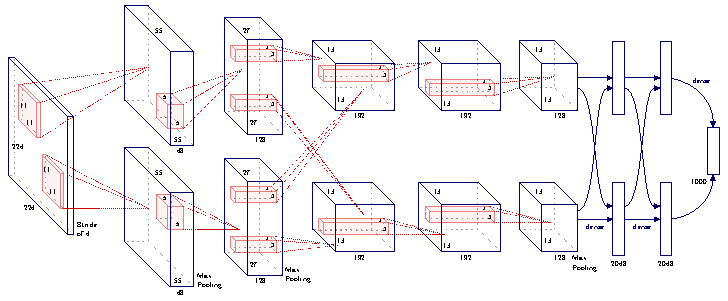
\includegraphics[width=\textwidth]{tikz/chapter5 - AlexNet.pdf}
    \caption{AlexNet Architecture}
\end{figure}

\textbf{Universal Feature Extractor}: AlexNet showed that features learnt from convolutional layers (features before the output layer, 4096 dimensional features for each image) can be generalised and reused effectively for a wide range of computer vision tasks, making it a universal feature extractor (as they become quite discriminative). Also, a study showed that features used in computer vision before AlexNet were way less discriminative even than features extracted after the first convolutional layer of the network. Finally, the features extracted from AlexNet are so powerful and discriminative that, when applied to another dataset (such as SUN-397) or to a different task from the original one, they produce \textbf{equally effective results without needing to be redefined or re-trained}.

\subsection{ILSVRC - Zeiler and Fergus Net (2013)}
ILSVRC 2013 introduced similar architecture to AlexNet (5 convolutional layers and 2 fully connected layer at the end each with 4096 units), but with some significant innovations. Its main features include:
\begin{itemize}
    \item Use of \textbf{smaller kernels in the first convolutional layers} (from 11x11 to 7x7).
    \item Use different number of channels. Why? Because their goal was to see visually what's happen inside a CNN.
    \item Introduction of the \textbf{explicability of CNNs through deconvolutional networks}.
    \item Article: \href{https://arxiv.org/pdf/1311.2901.pdf}{"Visualising and Understanding Convolutional Networks" (Zeiler and Fergus)}
\end{itemize}

In order to better understand what happens within a convolutional neural network and to identify the areas of interest on which it focuses to classify an image, we use \textbf{Deconvolutional Networks}. The work of Zeiler and Fergus is fundamental in this field and has made it possible to visualise activity in the intermediate layers of a CNN.

A Deconvolutional Network aims to interpret the activations in the various layers of a CNN by mapping them in pixel space. It works by reversing the convolution process: it is run in reverse and used as a probe without the need for learning. To do this, you \textbf{connect a Deconv Net to a layer of the CNN} you wish to probe, pass the input image through the CNN to obtain the activations, and then map these activations to pixel space.

\begin{figure}[!htbp]
    \centering
    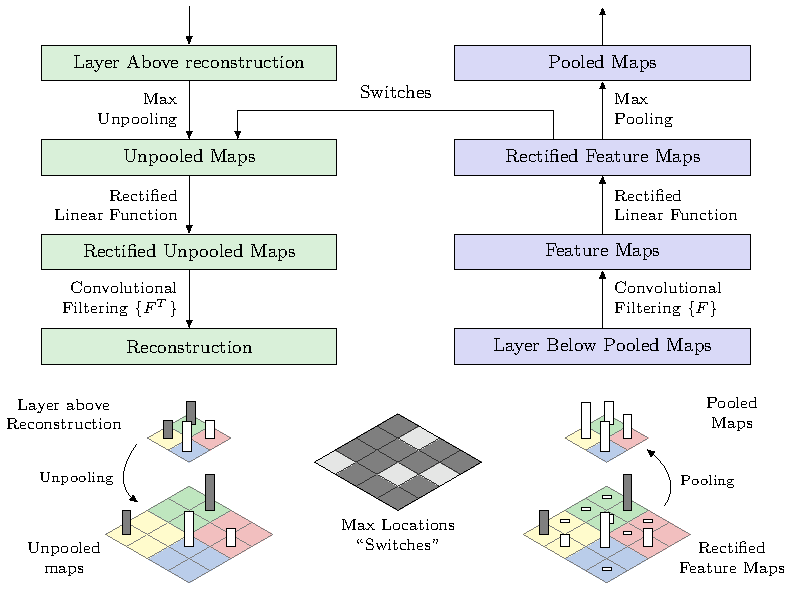
\includegraphics[width=0.9\textwidth]{tikz/chapter5 - Deconvolutional Networks.pdf}
    \caption{Functioning of a Deconvolutional Network with Unpooling}
\end{figure}

The deconvolution process includes several steps: unpooling, rectification and filtering. Unpooling is performed using \textbf{switch variables to keep track of the positions of the maxima in the original pooling}, as max pooling is not invertible. Rectification uses the ReLU function to propagate only non-negative values, while filtering applies transposed versions of the learned filters.

The result is a visualisation that shows which features of the original image were relevant for classification, allowing us to understand which patterns the algorithm found discriminative for a given class and better understand the inner workings of the CNN to improve its performance and interpretability.

\begin{figure}[!htbp]
    \centering
    \includegraphics[width=0.47\textwidth]{tikz/chapter5 - Deconvolutional Networks Captured Patterns}
    \caption{Patterns Captured in a Layer of a CNN}
\end{figure}

Another method to visualise whether the CNN is learning correctly is to \textbf{occlude an image at various positions} and observe the feature activations and classifier confidence. 

Zeiler and Fergus' principle is based on developing a scheme to interpret the internal behaviour of neural networks, and occlusion experiments are a useful tool in this context.

There are also other ways of visualising the inner workings of a CNN, such as \textbf{Class Model Visualisation}, introduced in \href{https://arxiv.org/pdf/1312.6034}{"Deep Inside Convolutional Networks: Visualising
Image Classification Models and Saliency Maps" (Simonyan et al.)}, which is a more rigorous approach than the alternative. Essentially, a model can be viewed as a function that generates a vector containing the predictions for each class, so its size depends on the number of classes. One could consider reversing the optimisation process within a CNN: instead of adjusting the weights of the neural network through back-propagation, the goal is to find an \textbf{image that maximises the score for a specific label}. 

However, two main challenges arise: different optimisers may produce different solutions and different optimisers may introduce distinct numerical optimisation problems. This final point is related to the fact that this approach requires the implementation of regularisation techniques.

An important technique introduced later to better understand how CNNs work is \textbf{Grad-CAM} (Gradient-weighted Class Activation Mapping), which \textbf{evidences relevant} regions of an image for classification.
It was introduced in the article \href{https://arxiv.org/pdf/1610.02391}{"Grad-CAM: Visual Explanations from Deep Networks via Gradient-based Localization" (Selvaraju et al.)}.

The intuition is that gradients of the classification score with respect to the final convolutional feature map are used to identify the parts of an input image that most influence the classification score. The places where this gradient is large are those where the final score is most dependent on the data.

To calculate the Grad-CAM, we proceed as follows:

\begin{itemize}
    \item The gradient of the score for the class \(c\) before softmax with respect to the feature maps of a convolutional level is calculated.
    \item A global pooling is performed on the obtained gradients.
\end{itemize}

\begin{figure}[!htbp]
    \centering
    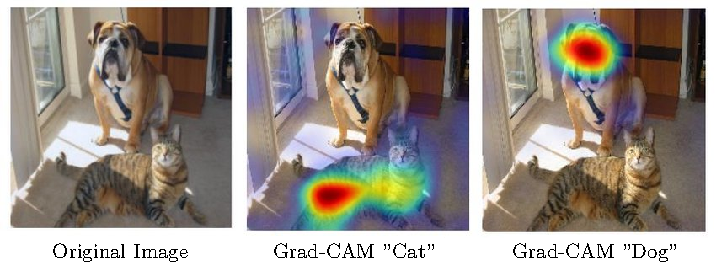
\includegraphics[width=0.7\linewidth]{tikz/chapter5 - GradCam.pdf}
    \caption{Grad-CAM applied to an Example Image}
\end{figure}

\subsection{VGGNet (2014)}
VGGNet represents an extension of the ideas introduced by AlexNet, with increased depth. It was the last NN developed with the AlexNet-like structure: alternation of convolutional layers and pooling layer until a small dimension is reached, and then attach a fully connected layer.

Its main features include:
\begin{itemize}
    \item Very deep architecture with \textbf{more than twice the parameters of AlexNet}.
    \item Keeps the sequence of convolutions, subsamples and layers fully connected.
    \item One of the first architectures to demonstrate that \textbf{network depth is a critical factor for performance}.
    \item Article: \href{https://arxiv.org/pdf/1409.1556.pdf}{"Very Deep Convolutional Networks for Large-Scale Image Recognition" (Simonyan and Zisserman)}
\end{itemize}

\begin{figure}[!htbp]
    \centering
    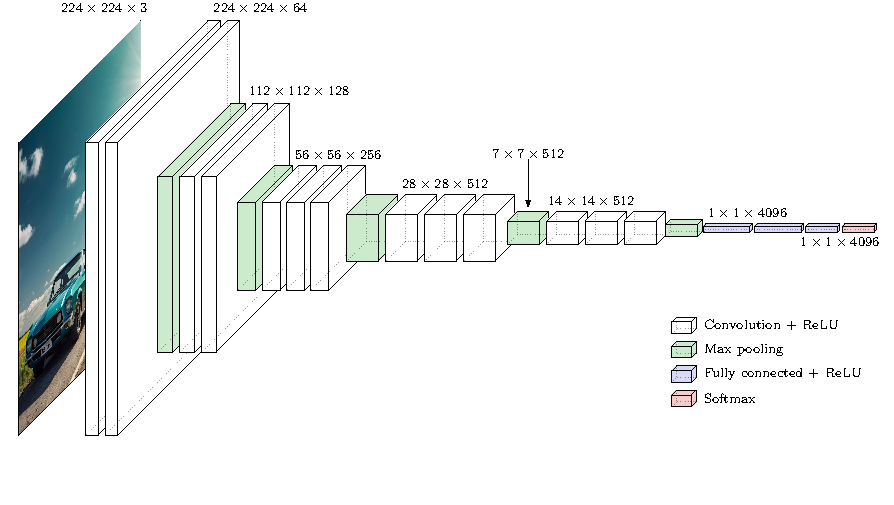
\includegraphics[width=0.7\textwidth]{tikz/chapter5 - VGGNet.pdf}
    \caption{VGGNet Architecture}
\end{figure}

\subsection{GoogleNet (2014)}
The primary issue with VGG was the exponential increase in the number of parameters. Subsequently, neural network architectures underwent a dramatic shift towards significantly reducing the number of parameters. This reduction was prompted by the recognition that the alternating architecture employed by AlexNet had become impractical. Instead of expanding the parameter count, the focus shifted towards increasing the number of layers (depth). A prominent example of this "new NN way" is GoogleNet, A 22-layer CNN but with a reduction in the number of parameters: from 60 million (AlexNet) to 4 million.

GoogleNet introduced an innovative structure, reducing the number of parameters compared to AlexNet. Its main features include:
\begin{itemize}
    \item Does not use fully connected layers, \textbf{reducing the complexity of the model} (inception module) and the risk of overfitting.
    \item Usage of supervision both at the end and intermidiate layers in order to fight with vanishing gradient (a deeper network is more prone to). 
    \item Usage of \textbf{inception modules}, allowing the network to capture details at different scales. An inception module consists of multiple convolutional layers with different kernel sizes, which are concatenated to capture features of different scales simultaneously. This parallelism helps GoogleNet capture fine-grained details as well as high-level features, making it exceptionally effective at image recognition tasks.
    \item Use of \textbf{1x1 convolutions to reduce the number of channels}, improving computational efficiency and reducing the computational workload.
    \item Introduction of \textbf{batch normalization}, which helps stabilise and speed up the training process. This is because if the inception block is trained with batch normalization, performance improves, even achieving the same performance as if not using batch normalization, but in fewer steps.
    \item Article: \href{https://arxiv.org/pdf/1409.4842.pdf}{"Going Deeper with Convolutions" (Szegedy et al.)}
\end{itemize}

\begin{figure}[!htbp]
    \centering
    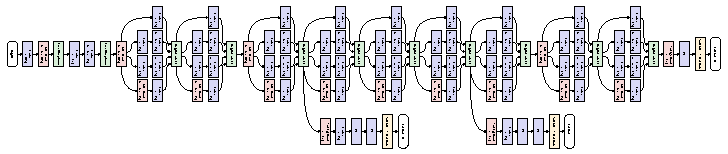
\includegraphics[width=\textwidth]{tikz/chapter5 - GoogleNet.pdf}
    \caption{GoogleNet Architecture}
\end{figure}



Furthermore, the same authors of this paper suggested some guidelines for designing deeper
architectures:

\begin{enumerate}
    \item \textbf{Avoid extreme compression}: When designing a deeper CNN, it is important not to over-compress the information from the previous layer. It is preferable to gradually reduce the size of the representation rather than doing so drastically.

    \item \textbf{Higher-dimensional representations are easier to process locally}: It means that within a network, it is easier to process representations that maintain a larger spatial dimension rather than compressing them too much.

    \item \textbf{Reduce the input size before spatial aggregation}: Using 1x1 filters to reduce the input size before combining spatial features can be done without significantly losing the representation.

    \item \textbf{Balancing the depth and width of Inception modules}: It is not yet completely clear how to best distribute the computation between height, width, and depth within an Inception module. However, it is advisable to look for an optimal balance to achieve good results.
\end{enumerate}

\subsection{ResNet (2015)}

Generally, if we have a NN with 18 layers and another with 34 layer, we would think that the last should perform better. Unfortunately, it is not the case and performance degradation is seen. ResNet addressed the problem of \textbf{performance degradation} of deep neural networks by introducing the idea of identity layers, also known as skip connection or identity bypass. Its main features include:
\begin{itemize}
    \item \textbf{Identity Layers}: allow the model to learn to ignore certain layers when they are not needed.
    \item Using \textbf{many small kernels}, reducing the overall number of parameters and improving computational efficiency.
    \item ResNet can be seen as the \textbf{implicit ensemble of more superficial neural networks}, thanks to skip connections. In fact, if we unrolled a connection encompassing a residual blocks, we would have multiple paths through the network.
    \item Skip connections make the \textbf{loss landscape much more uniform} and easier to optimise during the training process.
    \item Article: \href{https://arxiv.org/pdf/1512.03385.pdf}{"Deep Residual Learning for Image Recognition" (He et al.)}
\end{itemize}

\begin{figure}[!htbp]
    \centering
    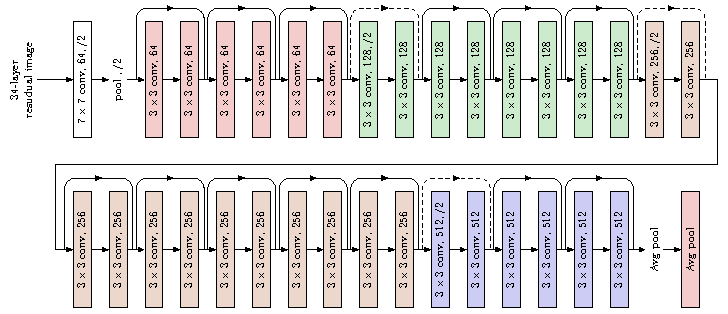
\includegraphics[width=\textwidth]{tikz/chapter5 - ResNet.pdf}
    \caption{ResNet Architecture}
\end{figure}

After ResNet, CNN designs did not used anymore final fully connected layers if the model is deeper enough. Also, batch normalization became the only method used as regularization method for CNNs, allowing removal/decrease of dropout and L2 regularization.

There are two remarkable architectures inspired by ResNet: 

\textbf{DenseNet} is an evolution of ResNet where each layer is directly connected to all other layers in the block. This promotes the reuse of features extracted from previous layers, improving gradient propagation and training stability. Advantages:
\begin{itemize}
    \item \textbf{Feature reuse}: Each layer receives input from all previous layers in the dense block, enabling efficient reuse of information.
    \item \textbf{Parameter reduction}: As each layer uses existing features, the need to learn new features from scratch is reduced, improving the overall efficiency of the network.
\end{itemize}

\textbf{SENet} (Squeeze-and-Excitation Network) improves ResNet by introducing Squeeze-and-Excitation blocks that adaptively recalibrate features based on channel importance. This is done by calculating a weight for each channel using a sigmoidal activation function. Advantages:
\begin{itemize}
    \item \textbf{Feature recalibration}: SE blocks compute weights for each channel, focusing on the most relevant ones, thus improving the network's ability to adapt to crucial details and patterns.
    \item \textbf{Performance improvement}: SENet has been shown to improve the accuracy of neural networks while reducing the number of parameters needed.
\end{itemize}

\subsection{ConvNeXt (2022)}
ConvNeXt represents a CNN architecture that has proven to be \textbf{competitive with modern transformers}. Its main features include:
\begin{itemize}
    \item Designed to compete with modern transformer models.
    \item Use of \textbf{connection structures between layers} that enable more effective learning of spatial and semantic relationships.
    \item Article: \href{https://arxiv.org/pdf/2201.03545.pdf}{"A ConvNet for the 2020s" (Liu et al.)}
\end{itemize}


\section{Regularisation Techniques for CNNs}
Convolutional Neural Networks have demonstrated excellent learning capability on a wide range of computer vision tasks. However, like many other machine learning techniques, CNNs are \textbf{susceptible to the phenomenon of overfitting}, in which the model overfits the training data, reducing its ability to generalise to new data.

To mitigate overfitting and improve the performance of CNNs, several specific regularisation techniques have been developed. In this section, we will examine some of these popular techniques: Cutout, Dropblock, Cutmix.

\begin{outline}
Cutout is a regularisation technique that consists of \textbf{cutting a random rectangular area of the input image} (16x16) during the training process. This cut region is subsequently filled with the average pixel value of the entire dataset. \textit{In practice, we force the model to consider more parts of the image during training, thus reducing the risk of overfitting.} \\

Dropblock is an extension of the dropout technique, in which instead of randomly deactivating certain neurons during training, \textbf{entire regions of neurons within a convolutional layer are deactivated}. This prevents the network from focusing too much on specific input features, promoting a more robust and general feature representation. Other variations are Dropout, drops individual values, and SpatialDropout, drops a whole channel.\\

Cutmix: During training, \textbf{a random rectangular area of an image is replaced with a corresponding area from another image}, while class labels are mixed in proportion to the replaced area. This technique encourages the model to learn useful features from multiple regions of the image, while providing a form of regularisation.
\end{outline}


\section{Object Detection}

Image classification is only one of the tasks that Convolutional Neural Networks can tackle. In addition to this, there are more complex tasks such as object detection, in which it is necessary not only to classify the objects in the image, but also to \textbf{identify their exact location through bounding boxes}. In this section, we will explore the strategies used to deal with this challenge using \textit{our beloved} CNNs.

Object detection is a complex task as it requires \textbf{both the classification of objects and the prediction of their positions through bounding boxes}. Thus, it implies doing simultaneously a classification and a regression task (for predicting continuous values, i.e. the bounding box). The input we provide is still an image, but the outputs are bounding boxes with labels for each object in the image. 

This approach makes the training of networks more difficult than simple classification, as there are problems such as data sparsity and difficulty in accurately locating objects. 

Before the advent of models such as AlexNet, the situation of object detection was at a standstill, with competition results stable on a plateau. However, the introduction of innovative techniques revolutionised this field.

\subsection{Selective Search for Object Recognition (2013)}
Selective Search is an image segmentation algorithm used to generate \textbf{proposed regions of interest} (RoI) for object recognition. The idea is to produce many "patches" in the image, and for each the algorithm assigns a likelihood score of that region containing the object of interest: regions with low likelihood are very unlikely to cointain it (and viceversa).

Its main features include:

\begin{itemize}
    \item \textbf{Groups similar pixels together to form regions} and combines them into larger segments.
    \item \textbf{Preliminary Step}: identifies possible areas of the image that might contain objects before proceeding with classification.
    \item Using a hierarchical approach, the algorithm groups pixels according to specific criteria to form a "tree", which is used to obtain bounding boxes.
    \item Article: \href{https://ivi.fnwi.uva.nl/isis/publications/2013/UijlingsIJCV2013/UijlingsIJCV2013.pdf}{"Selective Search for Object Recognition" (J.R.R. Uijlings et al.)}
\end{itemize}


\subsection{R-CNN - Region-based Convolutional Neural Network (2014)}
R-CNN is the \textbf{first convolutional neural network-based approaches for object recognition}. Its main features include:

\begin{itemize}
    \item \textit{It's nothing but Selective Search + AlexNet}.
    \item Use \textbf{proposed regions} to identify objects in the image.
    \item Uses a convolutional neural network to \textbf{extract features and classify objects within these regions}: We begin by taking an image and employing selective search to extract a set of region proposals ($\sim$2k/image). For each proposal, we fine-tune AlexNet individually, extracting features and training a classifier to determine whether the patch contains the target object.
    \item \textbf{Efficiency problem}: R-CNN uses a multi-stage model and Selective Search to explore the entire space of bounding boxes. Also, Selective Search is a "fixed" algorithm that does not dynamically adapt to the image, making it necessary to resize the input before passing it through the neural network, resulting in a \textbf{naive pipeline} approach. Lastly, both training and testing are very slow; for example, testing requires to rerun selective search, about 2k forward pass per images. Despite this, R-CNN performed significantly better than shallow models.
    \item Article: \href{https://arxiv.org/pdf/1311.2524.pdf}{"Rich feature hierarchies for accurate object detection and semantic segmentation" (Ross Girshick et al.)}
\end{itemize}

\begin{figure}[!htbp]
    \centering
    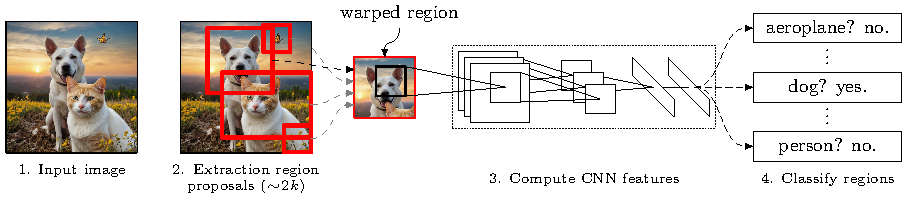
\includegraphics[width=\linewidth]{tikz/chapter5 - R-CNN.pdf}
    \caption{R-CNN Pipeline}
\end{figure}

\subsection{Fast R-CNN (2015)}
Fast R-CNN is an improved version of R-CNN that \textbf{addresses the efficiency issues} of its predecessor. Its main features include:

\begin{itemize}
    \item \textbf{Region of Interest (RoI) pooling}: Introduces a RoI pooling layer that allows the best use of the information extracted from the convolutional network for each proposed region. This level makes it possible to \textbf{reduce the size of the proposed regions as input} to the final classifier without loss of significant information.
    \item \textbf{Convolution of the forward pass of a CNN}: Fast R-CNN shares the forward pass of a CNN on the image across its selected sub-regions. This means that \textbf{convolution is performed only once} for the entire image, reducing the computational load and improving the overall efficiency of the model.
    \item Article: \href{https://arxiv.org/pdf/1504.08083.pdf}{"Fast R-CNN" (Ross Girshick)}
\end{itemize}

\begin{figure}[!htbp]
    \centering
    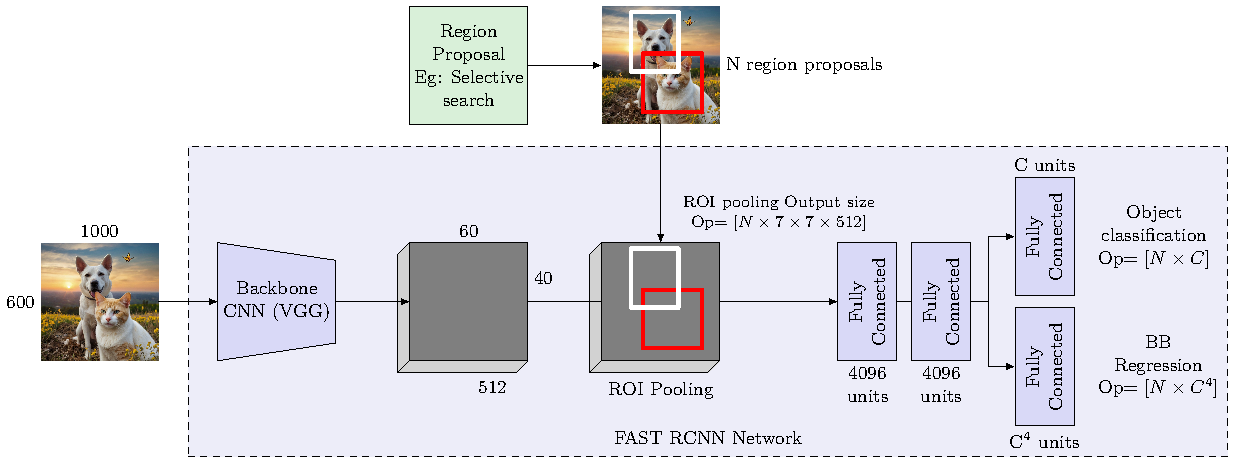
\includegraphics[width=\textwidth]{tikz/chapter5 - Fast R-CNN.pdf}
    \caption{Fast R-CNN Architecture}
\end{figure}


\subsection{Faster R-CNN (2015)}
Faster R-CNN is another significant development in the field of object detection. Differently to R-CNN and Fast R-CNN which use selective search to find out the region proposals, Faster R-CNN eliminates it as it is a slow and time-consuming process. Instead,  this model lets another the network to learn the region proposals. Its main features include:

\begin{itemize}
    \item \textbf{Similarity with Fast R-CNN}: Like Fast R-CNN, the image is provided as input to a CNN that provides a convolutional feature map.
    \item \textbf{Use of a separate network for proposal generation}: Instead of using Selective Search, a separate network called RPN (Region Proposal Network) is used in Faster R-CNN to predict region proposals. The predicted region proposals are then reshaped using a RoI pooling layer which is then used to classify the image within the proposed region and predict the offset values for the bounding boxes.
    \item \textbf{End-to-end architecture}: With the integration of the RPN module, Faster R-CNN allows the entire end-to-end model to be trained in a single step, improving efficiency and ease of training.
    \item Article: \href{https://arxiv.org/pdf/1506.01497.pdf}{"Faster R-CNN: Towards Real-Time Object Detection with Region Proposal Networks" (Shaoqing Ren et al.)}
\end{itemize}


\begin{figure}[!htbp]
    \centering
    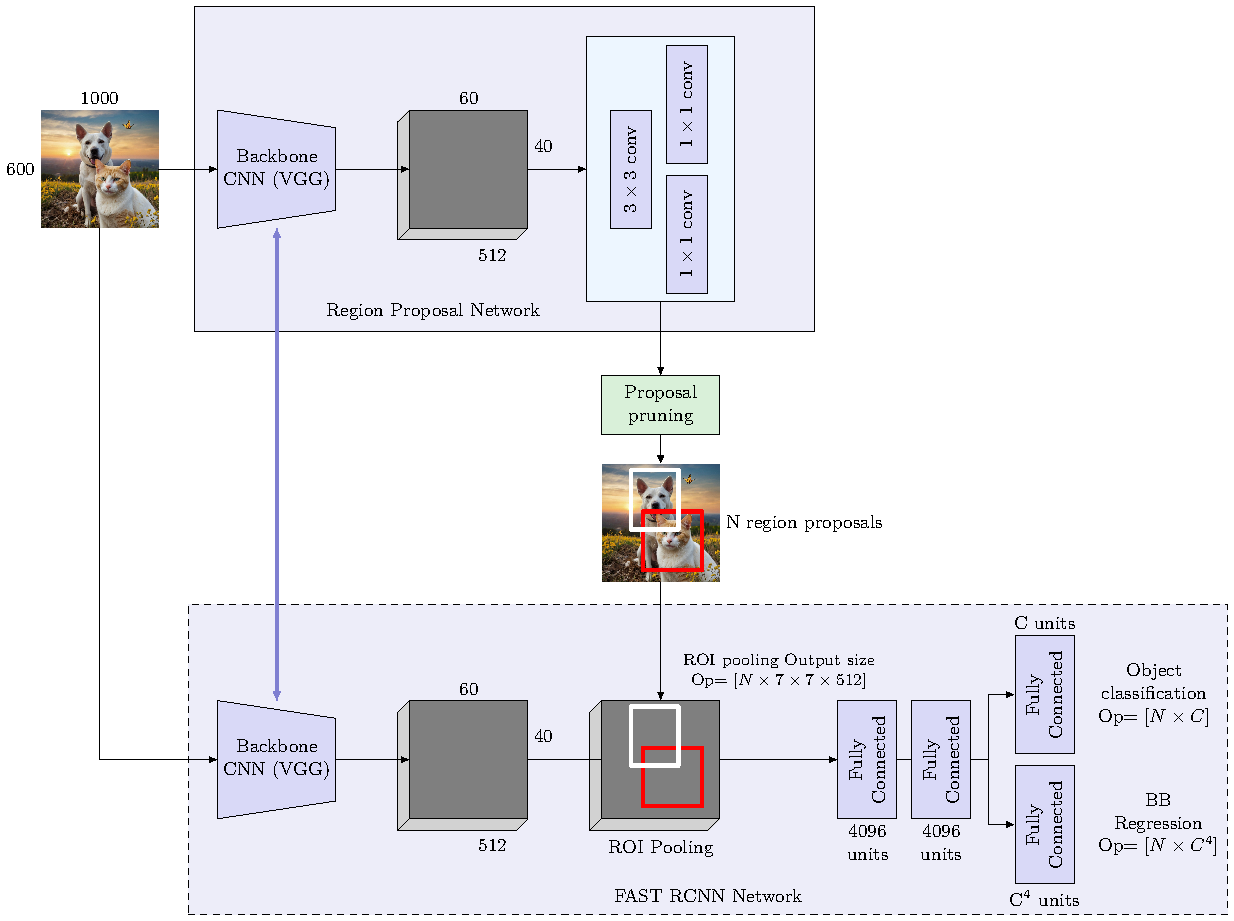
\includegraphics[width=\textwidth]{tikz/chapter5 - Faster R-CNN.pdf}
    \caption{Faster R-CNN Architecture}
\end{figure}



\subsection{YOLO - You Only Look Once (2016)}
YOLO is an innovative approach to object detection that \textbf{stands out for its speed and efficiency}. Its main features include:

\begin{itemize}
    \item YOLO treats the problem of object detection as a \textbf{direct regression problem}, in which the entire image is divided into a grid and for each grid cell the bounding box and class probability of the objects within that cell are directly predicted.
    \item \textbf{Use of a single convolutional network}: Unlike previous methods that use regions to locate objects in the image, YOLO uses a single convolutional network to predict bounding boxes and class probabilities for these boxes. This makes YOLO's approach simpler and more efficient.
    \item \textbf{Split image into grid}: YOLO splits the image into an SxS grid and for each grid cell predicts a set of bounding boxes. This approach allows YOLO to consider several regions of the image simultaneously.
    \item \textbf{Bounding box selection}: For each predicted bounding box, the YOLO grid produces a class probability and offset values for the bounding box. Bounding boxes with a class probability above a threshold are selected and used to locate the object in the image.
    \item Article: \href{https://arxiv.org/pdf/1506.02640.pdf}{"You Only Look Once: Unified, Real-Time Object Detection" (Joseph Redmon et al.)}
\end{itemize}

\begin{figure}[!htbp]
    \centering
    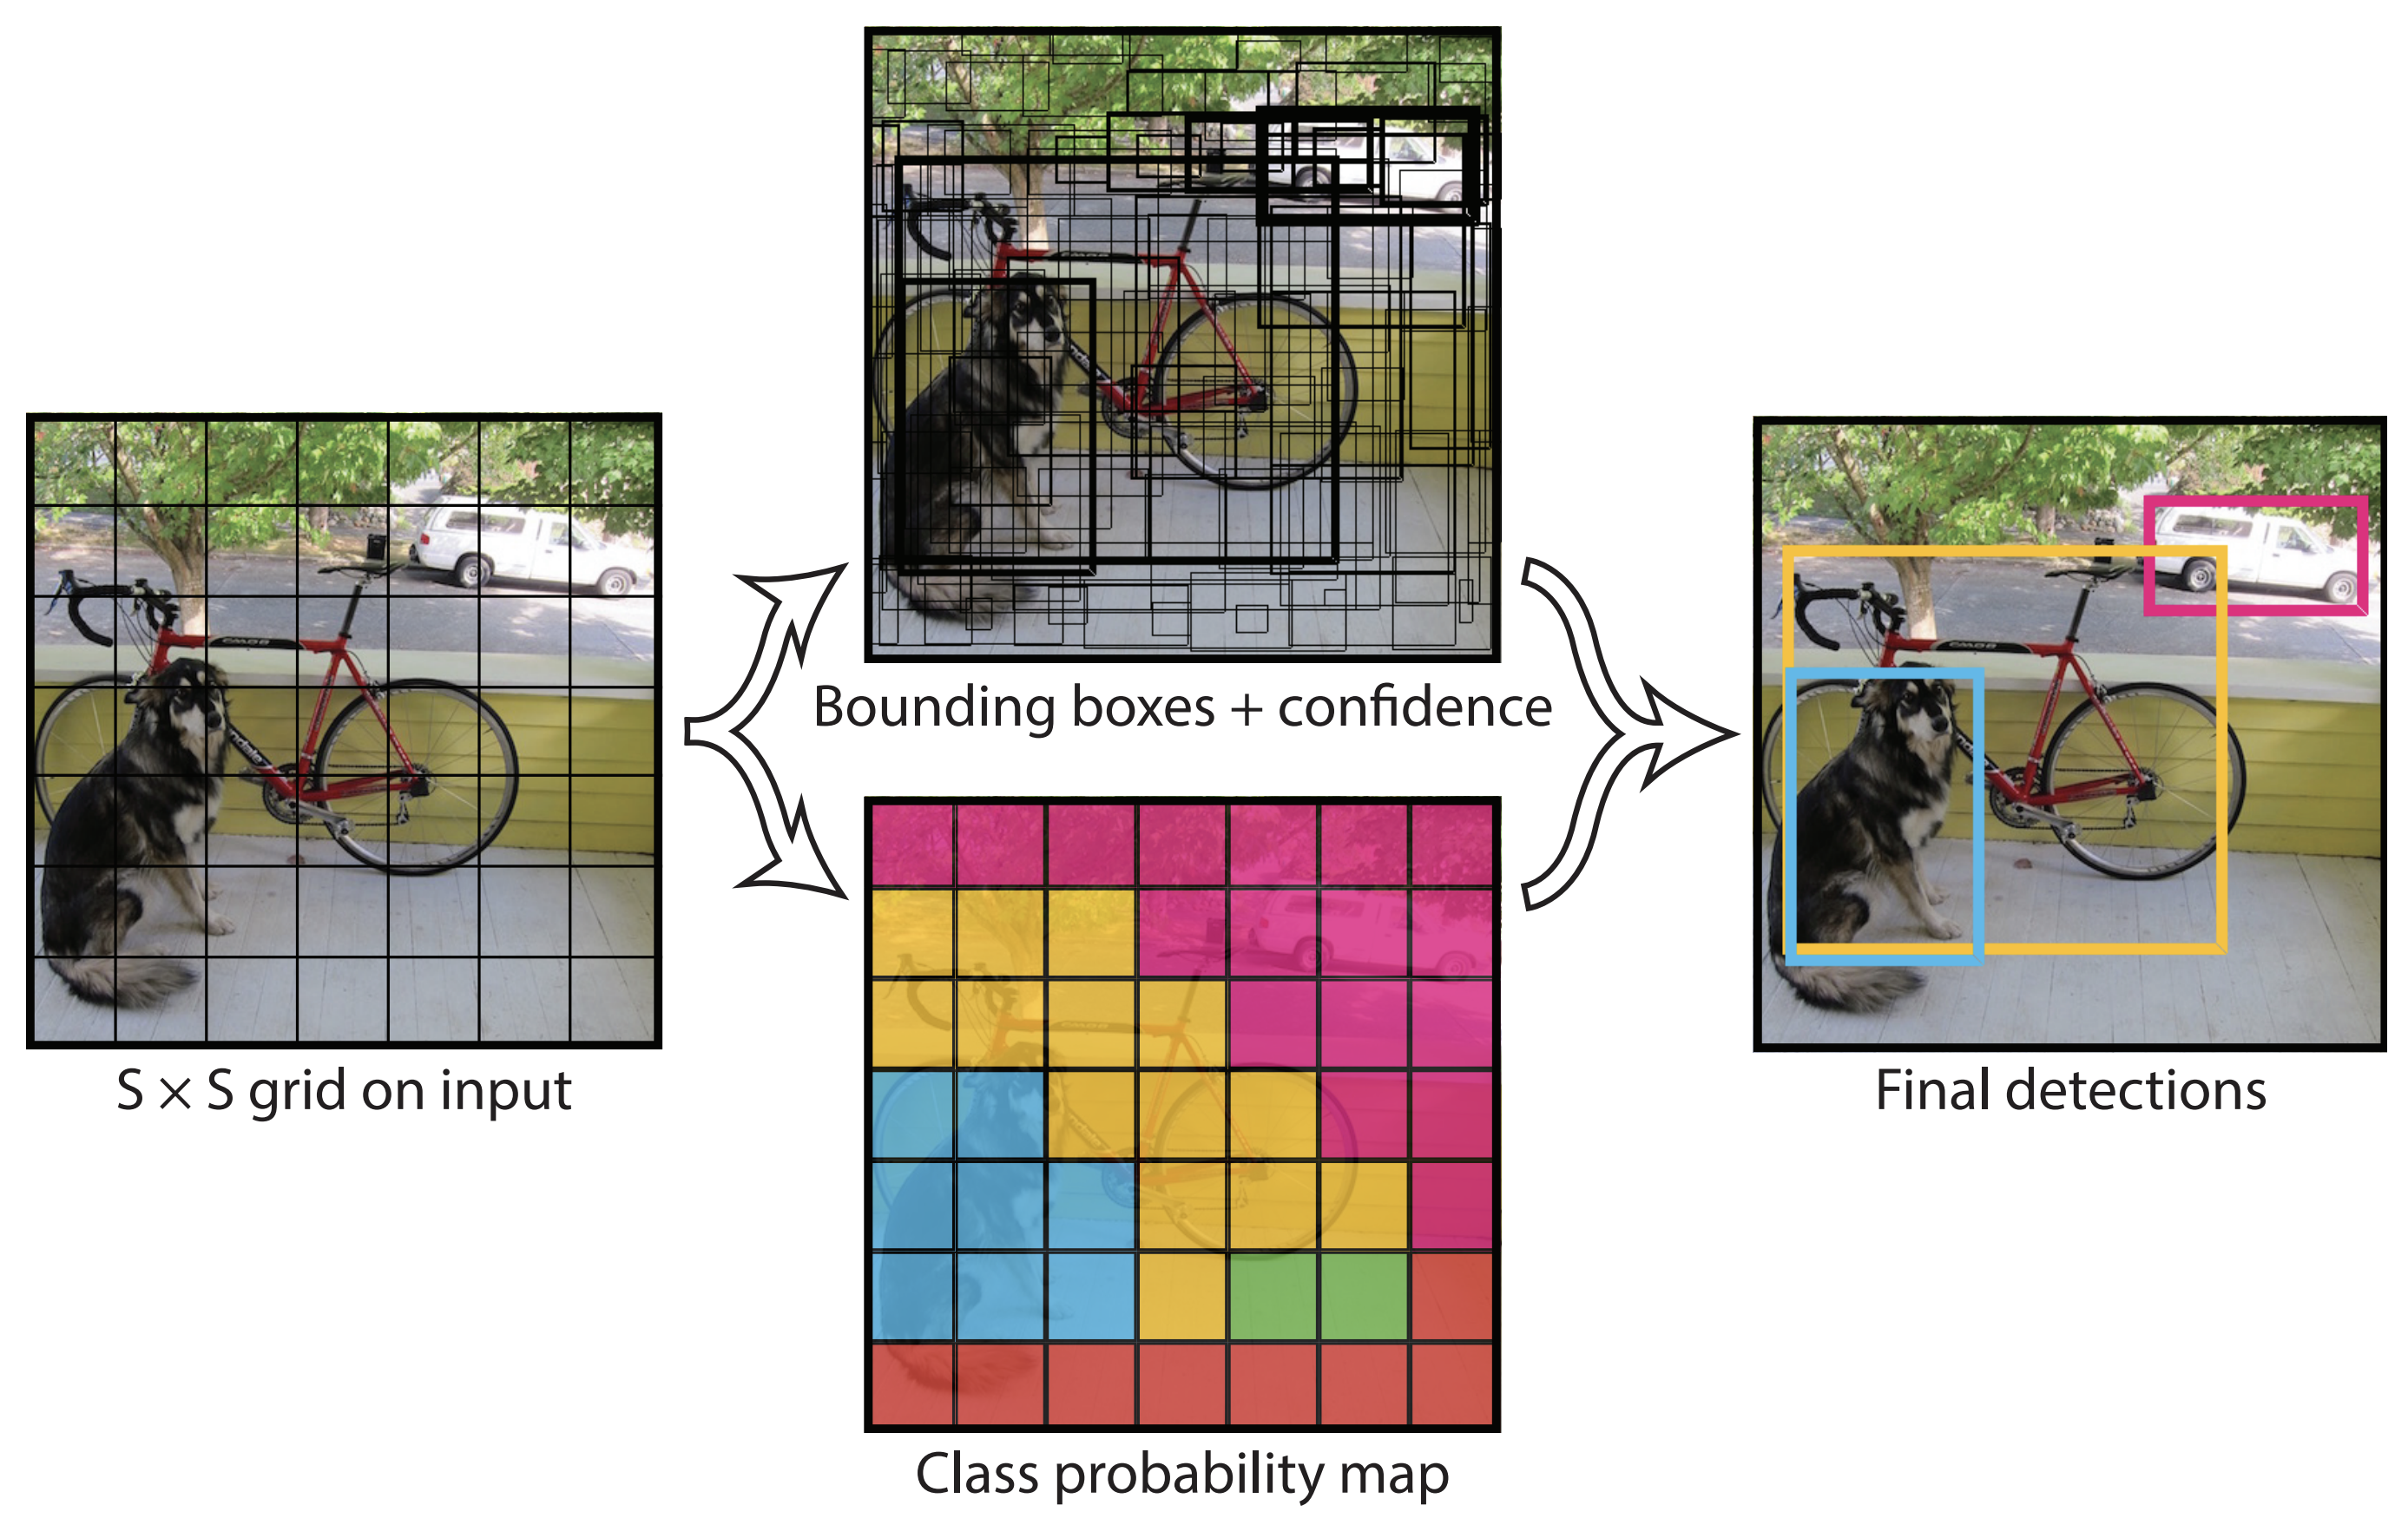
\includegraphics[width=\textwidth]{tikz/chapter5 - YOLO.png}
    \caption{YOLO Architecture}
\end{figure}

\section{Instance Segmentation}

In addition to object classification and bounding box detection, there is another challenge in computer vision: instance segmentation. It consists of \textbf{assigning a label to each pixel of an image}, distinguishing individual objects within the scene. This is an \textbf{even more complex challenge} than simple object detection, as it requires a detailed understanding of the structure and shape of the objects themselves.

One of the most advanced techniques to address this challenge is known as Mask R-CNN, which extends the Faster R-CNN framework for instance segmentation. 

\subsection{Mask R-CNN (2017)}

Mask R-CNN is an extension of Faster R-CNN that adds an \textbf{additional branch to the neural network for instance segmentation}. Its main features include:

\begin{itemize}
    \item Mask R-CNN uses \textbf{RoI Align}, an improved version of RoI Pooling, to ensure more precise alignment of feature maps during the instance segmentation phase. This significantly improves the quality of segmentation masks.
    \item \textbf{Pixel-level segmentation}: Mask R-CNN extends Faster R-CNN for pixel-level segmentation, allowing a label to be assigned to each pixel in the image based on the object instance to which it belongs.
    \item \textbf{FCN added}: Mask R-CNN adds a Fully Convolutional Network on top of selected features to produce accurate and detailed segmentation masks.
    \item Article: \href{https://arxiv.org/pdf/1703.06870.pdf}{"Mask R-CNN" (Kaiming He et al.)}
\end{itemize}



\newpage
\chapter{Recurrent Neural Networks}
\setbackgroundchapter{Recurrent Neural Networks}
\section{Handling Variable-Length Sequences}

So far we have mainly focused on models that handle \textbf{input and output of fixed size}. For example, in a convolutional neural network (CNN), we transform an input in the form of a matrix (image) into an output in the form of a vector (labels). However, the community has developed models that can handle variable-length structures, more specifically sequences, such as text, which is a sequence of strings.

Recurrent Neural Networks (RNNs) are flexible tools that can perform many different tasks, which can be classified as follows:

\begin{figure}[!htbp]
    \centering
    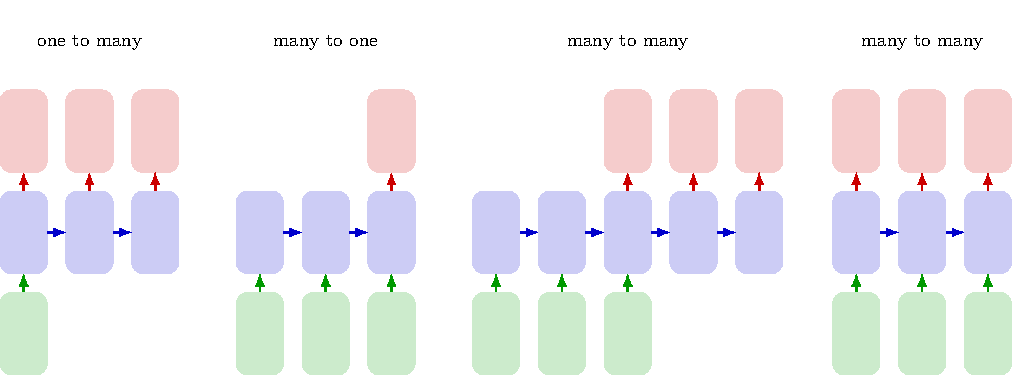
\includegraphics[width=\textwidth]{tikz/chapter6 - Types of RNN Models.pdf}
    \caption{Diagrams of RNN Models}
\end{figure}

\subsection{Multiple2Single: Sentiment Analysis}

In the sentiment analysis, the model must classify a product, restaurant, or any other item as positive, neutral, or negative based on the reviews received. In this scenario, we provide the neural network with inputs of varying sizes. Each word is transformed into a \textbf{hidden representation that reflects the context and propagates through subsequent words}, as these words are not independent of each other. This propagation occurs unidirectionally, similar to a feedforward neural network. However, the main difference is that instead of mapping a single input to an output of fixed size, the model takes multiple inputs and produces a single label. Predictions are typically made about the last hidden state, which should include the context of previous words.

\subsection{Single2Multiple: Image Captioning}

In image captioning, the network is fed a fixed input (an image), but the output will have a variable length, since we want to produce a sentence describing the content of the image. In this case, the latent representation of the image obtained from a CNN is \textbf{combined with the latent representations of the words to model the dependencies between them}. This approach allows a single input to be mapped to multiple outputs, generating several words that describe the image.

\subsection{Multiple2Multiple: Machine Translation}

In machine translation, the task is to translate a sentence from one language to another. This problem involves both multiple inputs and multiple outputs. Each word in the input sentence is mapped to a hidden representation that takes into account the context of the preceding words. The neural network uses these representations to generate the translated sentence, word by word, \textbf{maintaining sequential dependencies between words}. This allows the model to produce an accurate translation that reflects the meaning of the original sentence.

\section{Vanilla RNN}

Recurrent neural networks are, in essence, \textbf{neural networks with cycles}.

The Vanilla RNN, introduced in \href{https://www.sciencedirect.com/science/article/pii/036402139090002E}{"Finding structure in time" (Jeffrey L. Elman)}, has a \textbf{recurrent design} in that it performs the same parametric function for each input ($x_t$, each marked with a timestep), while the output ($h_t$, the hidden representation marked with the corresponding timestep) depends on the previous computation ($h_{t-1}$). After producing the output, this is \textbf{used to generate the hidden representation of the next RNN cell} ($h_{t+1}$). To make a decision ($y_t$), a linear layer can be applied to the end of a cell, considering both the current input and the output learned from the previous input.

There are two types of representations for an RNN: the \textbf{Folded} representation, which is synthetic, and the \textbf{Unfolded} representation, which provides a more explicit description of the computations. Below is the architecture of the network in both representations:

\begin{figure}[!htbp]
    \centering
    \includegraphics[width = 0.9\linewidth]{tikz/chapter6 - RNN Architecture.pdf}
    \caption{RNN Architecture}
\end{figure}

The structure of an RNN cell, as shown in the figure above, has two inputs ($x_t$ and $h_{t-1}$) and can be represented mathematically as follows:

$$
h_t = f_W(x_t,h_{t-1}) = \text{tanh} \ W \begin{pmatrix}
x_t \\
h_{t-1}
\end{pmatrix} = \text{tanh}(W_xx_t + W_hh_{t-1})
$$

In this equation, $h_t$ represents the hidden state at time $t$, $x_t$ is the input at time $t$, $h_{t-1}$ is the previous hidden state, $W_x$ and $W_h$ are the weights associated with the current input and previous hidden state respectively. The function $\text{tanh}$ provides nonlinearity to the network (\textit{Using hyperbolic tangent is understandable given that the paper is from the 1990s, a time when the use of it was common}). During training, $W$ weights are learned through the optimization process. For the prediction:
$$
y_t = \text{softmax}(W_y h_t + b_y)
$$
A peculiar aspect of RNNs is the \textbf{sharing of weights among different timesteps}: the weights $W_x$, $W_h$ and $W_y$ are shared between different timestep iterations, allowing the model to capture \textbf{sequential dependencies within the data}.

So, the main differences between an RNN and an FNN include the sharing of weights between timesteps, the use of backpropagation variation for training (in which we need to sum the contributions along the entire sequence) and the presence of three different sets of weights: $W_x$, $W_h$ and $W_y$. In addition, \textbf{the problem of gradient vanishing is more severe} in RNNs than in feedforward networks, mainly because of the hyperbolic tangent function used as the activation function. Also, backpropagation through time can be computationally expensive for a large number of timesteps.


\subsection{Truncated BPTT (Backpropagation Through Time)}


To solve the problems described above, we use the Truncated BPTT algorithm, which is a more efficient technique when dealing with long sequences. It was introduced as a Ph.D. thesis in \href{https://www.cs.utoronto.ca/~ilya/pubs/ilya_sutskever_phd_thesis.pdf}{"Training Recurrent Neural Networks" (Ilya Sutskever)}.

The idea of Truncated BPTT is to simplify this process. Instead of running the entire sequence through the network, we divide it into \textbf{smaller blocks of fixed length}. Each block is treated as a separate training unit. In this way, the network does not have to work with the whole sequence at once, but only with small chunks at a time, making training more efficient.

After presenting a block to the network, \textbf{backpropagation is performed only for a limited number of backward time steps}, rather than traversing the entire length of the sequence. This means that the network does not have to keep track of information too far back in time, reducing the computational cost of training.

To control how far back in time to go during backpropagation, we use two parameters, $k_1$ and $k_2$. The first, $k_1$, determines the \textbf{length of the blocks} into which we divide the sequence, while $k_2$ defines the \textbf{number of time steps} over which to perform backpropagation within each block. The Truncated BPTT algorithm can be schematized as follows:

\begin{algorithm}
\renewcommand\thealgorithm{}
\caption{}
\begin{algorithmic}[1]
\STATE Present a sequence of $k_1$ timesteps of input and output pairs to the network.
\STATE Unroll the network then calculate and accumulate errors across $k_2$ timesteps.
\STATE Roll-up the network and update weights.
\STATE Repeat the process.
\end{algorithmic}
\end{algorithm}
Adjusting $k_1$ and $k_2$ allows us to balance the training speed and the network's ability to capture long-range time dependencies.

\section{Long Short-Term Memory (LSTM)}

It has been recognized that the classical RNN suffers from an inefficient design in its individual cell, as efforts to improve learning have not produced significant improvements in the vanishing gradient problem due to inherent limitations in the cell design. To solve this problem, LSTM was introduced. The architecture was first presented in this article: \href{https://deeplearning.cs.cmu.edu/F23/document/readings/LSTM.pdf}{"Long Short-term Memory" (Sepp Hochreiter)}.

The LSTM cell not only produces the hidden state $h_t$, but adds another component called \textbf{Memory Cell} ($c_t$), which is responsible for maintaining and deleting information, based on the input context. This means that \textbf{some of the previous information must be remembered, some must be forgotten, and some new information must be added to memory}. Here is the design of the cell:

\begin{figure}[!htbp]
    \centering
    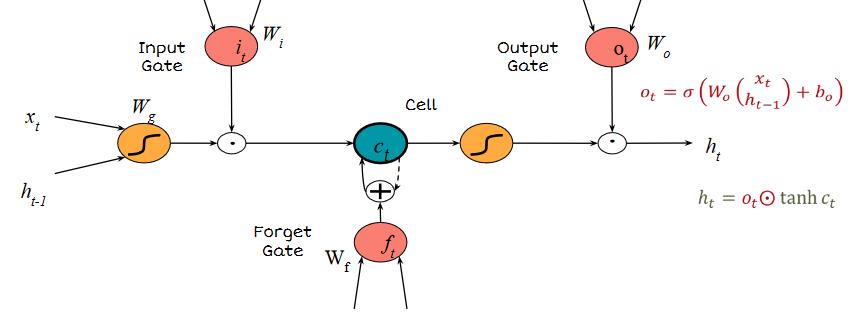
\includegraphics[width=\linewidth]{tikz/chapter6 - LSTM.png}
    \caption{{\color{red}\colorbox{pink}{Tikz TO-DO}} LSTM Cell Structure}
\end{figure}

As you can see, within an LSTM cell, there are three different parametric components, called \textbf{Gate}. Let's explore them in detail.

\begin{remark}{mybluee}{mybluee!20}
\textbf{Input Gate}: can allow the input signal ($x_t$ and $h_{t-1}$) to alter the state of the memory cell or block it.

Its output $i_t$ is computed by the sigmoid function applied to the input $x_t$ and the preceding dependency $h_{t-1}$, and is associated with its own parameters $W_i$:
$$ i_t = \sigma(W_i
\begin{pmatrix}
x_t \\
h_{t-1}
\end{pmatrix} + b_i)
$$

$i_t$ is used as a trade-off between the information passing through the current input ($x_t$ and $h_{t-1}$) and the information encoded by the previous cell ($c_{t-1}$).
\end{remark}

\begin{remark}{myred}{myred!20}
\textbf{Forget Gate}: can modulate the self-recurrent connection of the memory cell, allowing the cell to remember or forget its previous state as needed.

Its output $f_t$ is computed by the sigmoid function applied to the input $x_t$ and the previous dependency $h_{t-1}$, and is associated with its own parameters $W_f$:
$$ f_t = \sigma(W_f
\begin{pmatrix}
x_t \\
h_{t-1}
\end{pmatrix} + b_f)
$$
\end{remark}


\begin{remark}{accent}{accent!5}
\textbf{Memory Cell Calculation} is a combination of the previous two gates:
$$c_t = \textcolor{myred}{f_t} \odot c_{t-1} + \textcolor{mybluee}{i_t} \odot g_t $$

We can interpret the equation as follows:
\begin{itemize}
    \item \( \textcolor{myred}{f_t} \odot c_{t-1}\): The forget gate decides how much of the cell's previous state \( c_{t-1} \) should be forgotten or retained for the next state \( c_t \).
    
    \item \( \textcolor{mybluee}{i_t} \odot g_t \): This determines how much of the new information \( g_t \), i.e., the value of the input modulation, should be added to the state of the cell \( c_t \).
\end{itemize}
In short, \textbf{\textcolor{myred}{the forget gate modulates how much of the previous state to retain}}, while \textbf{\textcolor{myblue}{the input gate modulates how much of the new information is to be added to the cell state}}.
\end{remark}

\begin{remark}{mygreen}{mygreen!20}
\textbf{Output Gate}: can allow the state of the memory cell ($c_t$) to have an effect on other neurons, thus affecting the output of the LSTM unit ($h_t$).

First, a sigmoid layer decides which parts of the cell state ($c_t$) the model is going to produce as output (associated with its parameters $W_o$):
$$ o_t = \sigma(W_o
\begin{pmatrix}
x_t \\
h_{t-1}
\end{pmatrix} + b_o)
$$
\end{remark}

\begin{remark}{accent}{accent!5}
To \textbf{Calculate the Output} of the cell, a tanh layer is used on the state of the memory cell to shrink values between -1 and 1, which are then multiplied by the output of the output gate:
$$h_t = \textcolor{mygreen}{o_t} \odot \text{tanh}(c_t) $$
\end{remark}

It is important to note that although there are many nonlinearity functions, the calculations to update the value of the cell ($c_t$) are \textbf{linear}, so the gradient flow from $c_t$ to $c_{t-1}$ involves only \textbf{backpropagation through addition and element-by-element multiplication}, not multiplication of matrices or nonlinear functions.

We can also formulate a (\textit{beautiful}) compact version of everything we have seen, summarizing the formulas in:
$$
\setlength{\arraycolsep}{5pt}
\renewcommand{\arraystretch}{0.95}
\begin{pmatrix}
g_t \\
\textcolor{mybluee}{i_t} \\
\textcolor{myred}{f_t} \\
\textcolor{mygreen}{o_t} 
\end{pmatrix} = 
\begin{pmatrix}
\text{tanh} \\
\sigma \\
\sigma \\
\sigma 
\end{pmatrix}
\begin{pmatrix}
W_g \\
\textcolor{mybluee}{W_i} \\
\textcolor{myred}{W_f} \\
\textcolor{mygreen}{W_o}
\end{pmatrix}
\begin{pmatrix}
x_t \\
h_{t-1}
\end{pmatrix}
$$
$$c_t = \textcolor{myred}{f_t} \odot c_{t-1} + \textcolor{mybluee}{i_t} \odot g_t $$
$$h_t = \textcolor{mygreen}{o_t} \odot \text{tanh}(c_t) $$

\section{Gated Recurrent Unit (GRU)}
As the community began to apply LSTM models to various tasks such as captioning, it became apparent that the network was overly complex. Thus, thanks to \href{https://arxiv.org/pdf/1406.1078}{"Learning Phrase Representations using RNN Encoder–Decoder
for Statistical Machine Translation" (Cho et al.)}, the GRU network was introduced to address this complexity by simplifying the LSTM cell by \textbf{removing one of its gates}. Despite having only two gates, the model is sufficiently resilient to the vanishing gradient problem. Moreover, the information flow is stored only in the hidden state $h_t$. Here is the architecture of a cell:

\begin{figure}[!htbp]
    \centering
    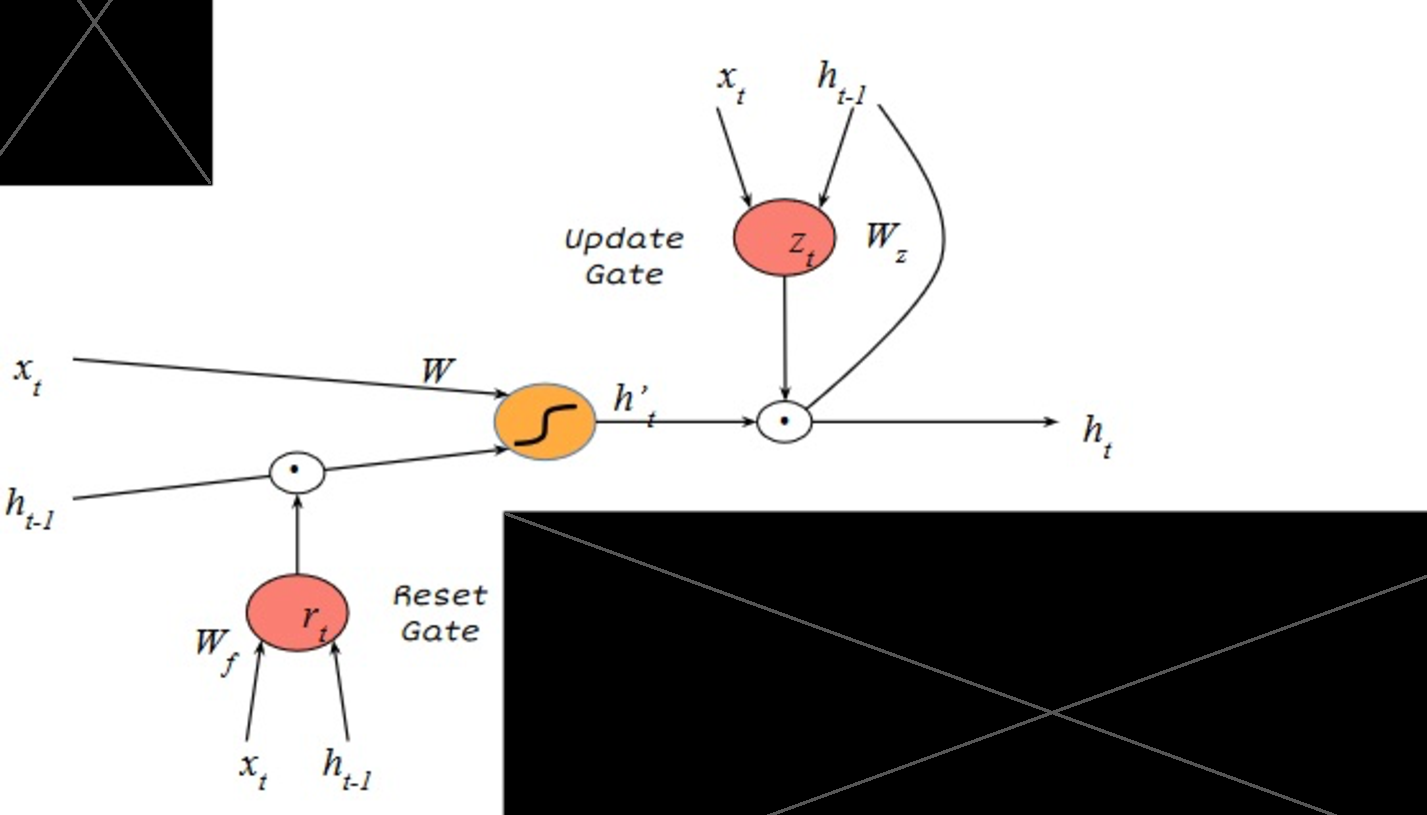
\includegraphics[width=0.85\linewidth]{tikz/chapter6 - GRU.pdf}
    \caption{{\color{red}\colorbox{pink}{Tikz TO-DO}} GRU Cell Structure}
\end{figure}

As before, let's analyze together the gates used in the GRU model.

\begin{remark}{myorange}{myorange!20}
\textbf{Reset Gate}: used to decide how much of the passed information to forget.

The output $r_t$ is computed by the sigmoid function applied to the input $x_t$ and the previous hidden state $h_{t-1}$, and is associated with its own parameters $W_r$:
$$ r_t = \sigma(W_r
\begin{pmatrix}
x_t \\
h_{t-1}
\end{pmatrix} + b_t)
$$
\end{remark}

\begin{remark}{accent}{accent!5}
An important change in the design of the LSTM cell is that \textbf{the value of the input modulation is no longer based solely on the complete information from the previous hidden state} $h_{t-1}$, but instead on a "restricted stream" determined by $\textcolor{myorange}{r_t}$:

$$ h'_t = \text{tahn }W(
\begin{pmatrix}
x_t \\
\textcolor{myorange}{r_t} \odot h_{t-1}
\end{pmatrix})
$$
\end{remark}

\begin{remark}{myyellow!85!black}{myyellow!20}
\textbf{Update Gate}: helps the model determine how much of the past information (from previous time steps) needs to be transmitted to the future.

The output $z_t$ is computed by the sigmoid function applied to the input $x_t$ and the previous hidden state $h_{t-1}$, and is associated with its own parameters $W_z$:

$$ z_t = \sigma(W_z
\begin{pmatrix}
x_t \\
h_{t-1}
\end{pmatrix} + b_z)
$$
\end{remark}


\begin{remark}{accent}{accent!5}
The \textbf{Final Representation of the Hidden State} is calculated by an additional point product:

$$h_t = (1-\textcolor{myyellow!85!black}{z_t})\odot h_{t-1}+\textcolor{myyellow!85!black}{z_t} \odot h'_t$$
\end{remark}


\newpage
\chapter{Sequence Models}
\setbackgroundchapter{Sequence Models}
\section{Introduction}

As the scientific community began to address problems involving sequentially structured data, RNNs returned to the forefront, leading to the development of new designs such as GRUs. However, it became apparent that RNNs had difficulty handling very long sequences. To address this problem, the Attention model was introduced as an auxiliary module, significantly improving performance in complex tasks such as image captioning and neural machine translation.

The concept of the Attention model initially found application in models that combined CNN and RNN, and then was incorporated into Transformers, the model underlying tools such as ChatGPT. This led to the emergence of an inevitable question, "\textit{Do we really need RNN and Attention models together for sequencing tasks, or can one Attention model suffice on its own?}" This question prompted the exploration of sequence models without the use of RNNs.

In this section, we will explore how this change came about through innovations implemented in the \textbf{Image Captioning} and \textbf{Machine Translation} tasks.


\section{Caption Model}

\subsection{Show and Tell}
Image captioning is the process of generating a textual description for given images. It can be seen as a Sequence to Sequence problem from beginning to end, where images, considered as sequences of pixels, are transformed into sequences of words. This task requires processing both textual and image statements. For the textual part, we use recurrent neural networks (RNNs) and for the visual part, we use convolutional neural networks (CNNs) to obtain feature vectors. Specifically, the architecture developed by Google in 2014 in the paper \href{https://arxiv.org/pdf/1411.4555}{"Show and Tell: A Neural Image Caption Generator" (Bengio et al.)} uses both GoogleNet and LSTM.

The procedure begins with feature extraction of the image using GoogleNet, which produces a feature vector, denoted as $I$. This vector is then inserted into the LSTM sequence at time $t=-1$, only once. Next, starting at $t=0$, a sequence of word vectors is inserted. Each word is represented as a one-hot vector $S_t$ with dimensions equal to the size of the vocabulary.

At each time step, the word vector $S_t$ is transformed through an embedding layer $W_e S_t$ and provided to the LSTM. Then, the input is processed along with the previous hidden state to produce a new hidden state and calculate the probability $p_t$ of the next word in the sequence. The word with the highest probability, denoted as $\log p_t(S_{t+1})$, is chosen as the output for that time step. This process is repeated until a special end-of-sentence word ($S_N$) or a maximum length of the sequence is reached. Check the image below for a visual representation of the process:
\newpage

\begin{figure}[!htbp]
    \centering
    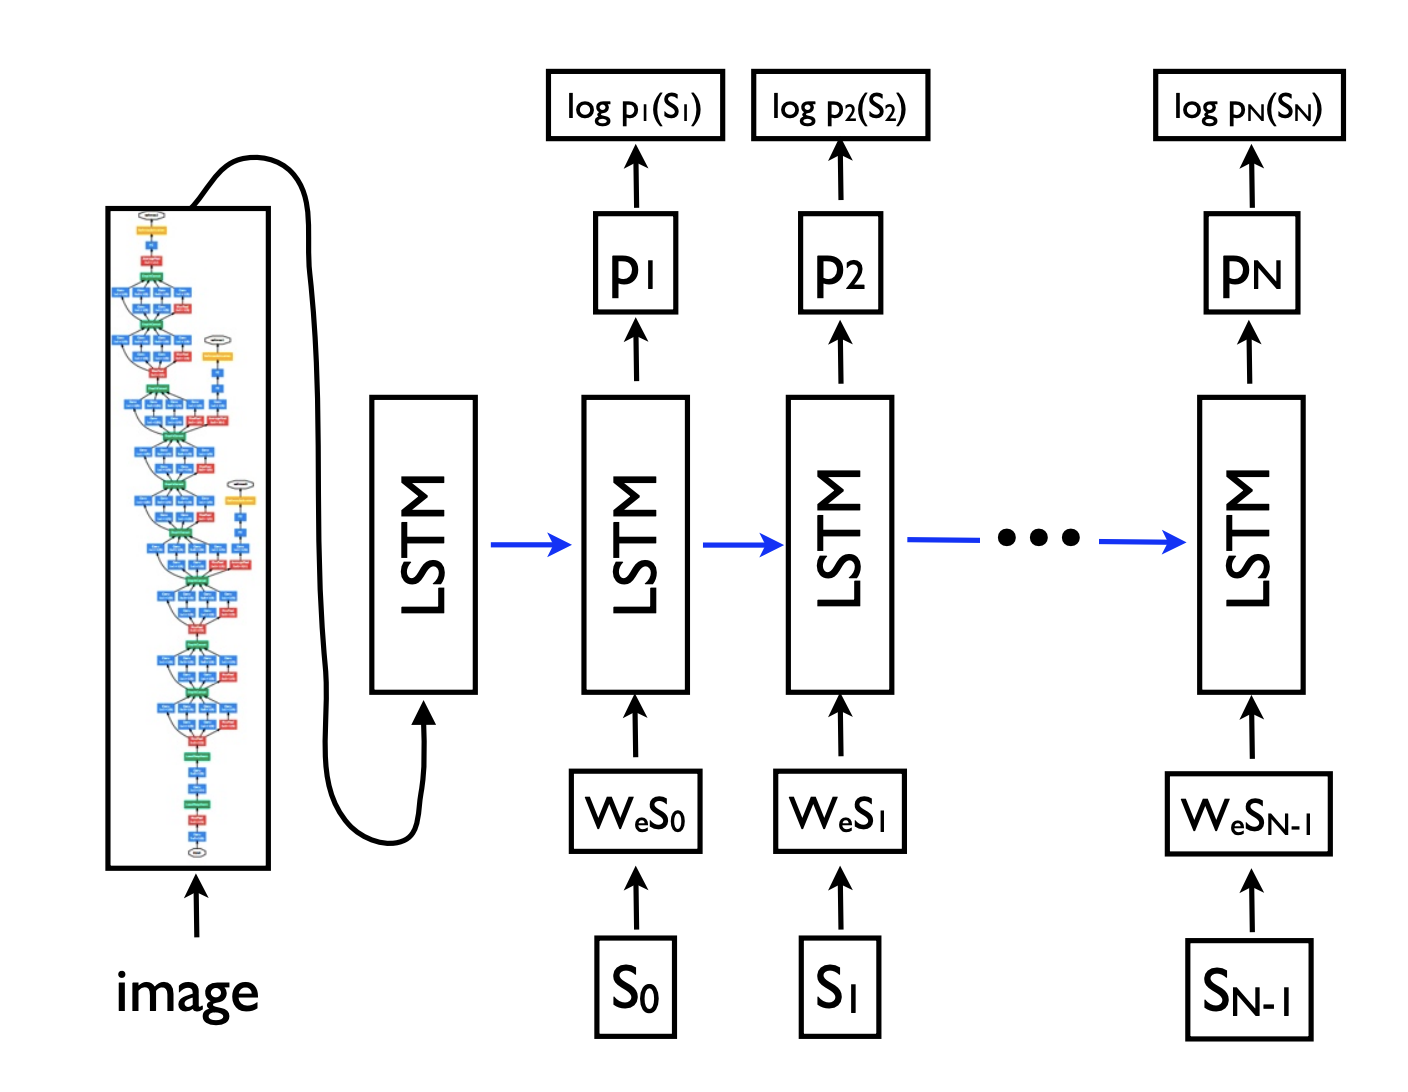
\includegraphics[width=\linewidth]{tikz/chapter7 - Show and Tell Model.png}
    \caption{{\color{red}\colorbox{pink}{Tikz TO-DO}} Show and Tell Caption Model}
\end{figure}

The quality of the generated caption depends strongly on the performance of the CNN, making fine-tuning crucial. So, the architecture combines CNN and LSTM in a way that leverages the visual feature extraction capabilities of CNN and the sequential modeling capabilities of LSTM to generate accurate and consistent captions for images.

For inference time, the model uses one of the following methods: \textbf{Sampling} and \textbf{Beam Search}.

In the sampling method, the first word is extracted according to a probability $p_1$, then the corresponding embedding is provided as input and the next word is extracted with probability $p_2$ (which depends on the probability that a certain word has been predicted previously). This process continues until the special end-of-sentence token is extracted or a maximum length is reached.

\begin{figure}[!htbp]
    \centering
    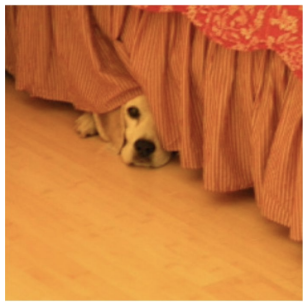
\includegraphics[width=\linewidth]{tikz/chapter7 - Sampling.png}
    \caption{{\color{red}\colorbox{pink}{Tikz TO-DO}} Sampling Visual Example}
\end{figure}

With Beam Search, on the other hand, we iteratively consider the \textbf{$k$ best sentences up to time $t$} as candidates to generate sentences of length $t+1$, keeping only the $k$ best of them. This approach allows more word combinations to be explored, improving the quality of the generated sentences compared to simple sampling.

\begin{figure}[!htbp]
    \centering
    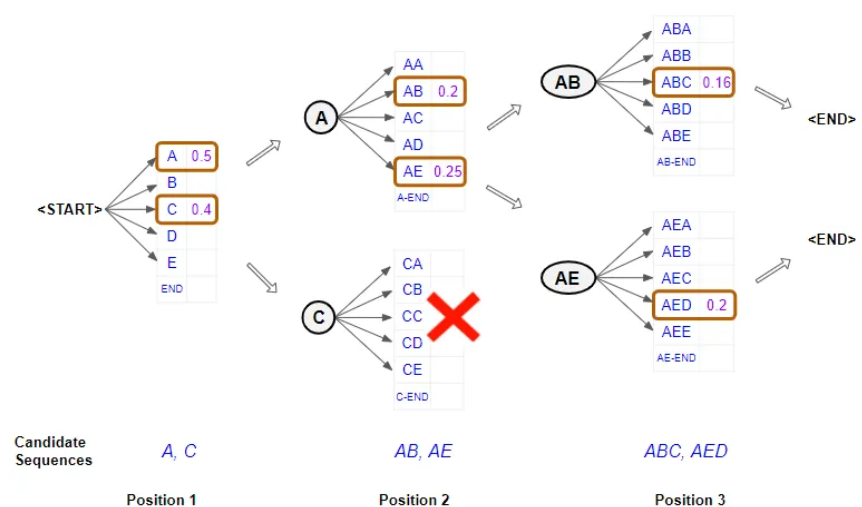
\includegraphics[width=\linewidth]{tikz/Beam Search.png}
    \caption{{\color{red}\colorbox{pink}{Tikz TO-DO}} Beam Search Visual Example}
\end{figure}

In the image above you can see an example of Beam Search with a width of 2, using characters for simplicity. Here's the description of what is happening:
\begin{itemize}
    \item \textbf{First Position}: The model starts with the token "<START>" and calculates the probabilities for each possible word. It selects the two characters with the highest probability, for example "A" and "C". 
    \item \textbf{Second position}: The model generates the probabilities for the second position twice, holding the first position ("A" or "C") constant. It then chooses the two best pairs of characters based on the combined probability, such as "AB" and "AE."
    \item \textbf{Third position}: This process is repeated. The model calculates the probabilities for the third position, limiting the first two positions to "AB" or "AE," and selects the best three combinations of characters based on the combined probability of the first three characters. This continues until a token "<END>" is selected, marking the end of that branch of the sequence. Simple, isn't it? \faSmile[regular]
\end{itemize}

In order to test the performance of the model, we face the challenge of comparing the output of the model with the \textbf{captions of human annotators}. Of course, the annotations of different individuals may vary, presenting inherent discrepancies. To address this problem, the Bilingual Evaluation Understudy (BLEU) score was used.

\subsection{BLEU Score}

The BLEU score is a metric used to evaluate the quality of texts generated in natural language processing (NLP) models. The text generated by the model is called \textbf{Candidate}, while the possible correct texts are called \textbf{References}. The BLEU score compares the candidate with the references to measure their similarity.

The BLEU score ranges from 0 to 1 and is based on accuracy, i.e., the \textbf{proportion of matching n-grams with references} (sequences of n words) found in the candidate compared \textbf{to the total number of n-grams in the candidate}. Usually, n-grams of size 1 to 4 are considered.

To prevent the candidate from scoring well by repeating the same n-gram many times, we \textbf{limit the number of occurrences} of each n-gram in the references. For example, if a reference contains the word "the" twice, the candidate should also not have more than two occurrences of "the".

Finally, the BLEU score is multiplied by a \textbf{brevity penalty} to prevent translations that are too short from getting high scores. 

Example:

\; The Reference is: "\textit{Transformers: Transformers make everything quick and efficient.}" 

\; The Candidate is: "\textit{Transformers Transformers Transformers Transformers.}" \ \img{tikz/chapter7 - Optimus Prime.png}
 
The BLEU score is low because the candidate repeats "Transformers" without providing full context, while the reference has a meaningful sentence. 

\section{Captioning with Attention}

\subsection{Show, Attend and Tell}

Captioning with attention represents a significant innovation in the field, especially for image and text processing. This approach, which was introduced in the paper \href{https://arxiv.org/pdf/1502.03044}{"Show, Attend and Tell: Neural Image Caption Generation with Visual Attention" (Xu et al.)} in 2015, has overcome some limitations of previous models, paving the way for more advanced results in image processing and caption generation.

The key idea of this approach is the integration of two key components: a convolutional neural network (CNN) for image feature extraction and a recurrent neural network (RNN) with an attention mechanism to generate captions. This combination allows the model to \textbf{focus attention on specific parts of the image while generating the corresponding description}.

The main innovations introduced by this approach are as follows:

\begin{itemize}
    \item \textbf{Feature Extractor}: A CNN is used to extract a set of feature vectors, each of which represents a part of the image. So, here we maintain the spatial information.
    \item \textbf{RNN with Attention}: The extracted feature maps are not only used for initializing the RNN, but are passed to each cell of the RNN during caption generation. This approach allows the network to focus attention on specific parts of the image as it generates each caption word. Each RNN cell produces both the probability of the predicted word ($p(y_t)$) and an attention map ($\alpha_t$) indicating the relevant parts of the image.
\end{itemize}

\begin{figure}[!htbp]
    \centering
    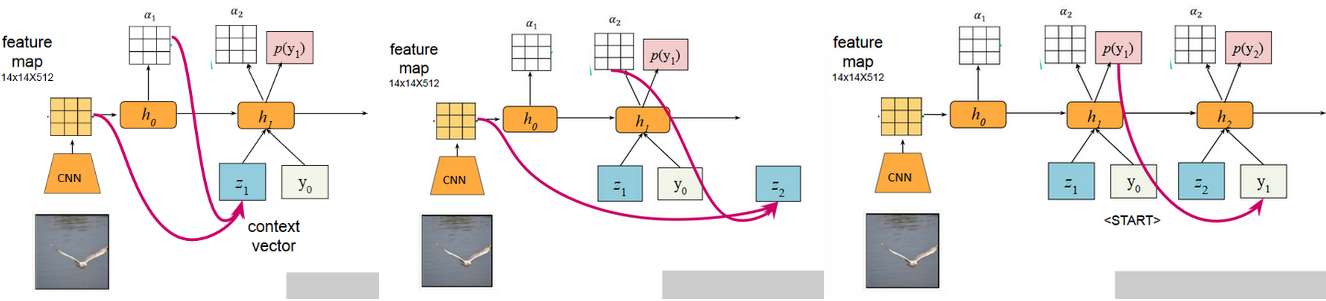
\includegraphics[width=1\linewidth]{tikz/Attention Model.png}
    \caption{{\color{red}\colorbox{pink}{Tikz TO-DO}}  Flow of Show, Attend and Tell}
\end{figure}

In the image above, each LSTM cell receives \textbf{three} main inputs: the previous latent space $h_{t-1}$, the predicted word in the current sequence $ y_{t-1} $ and a context vector $ z_{t} $ (obtained from the dot product between the feature map produced by the CNN and the previous attention map $\alpha_{t-1}$). 

\subsection{Types of Attention}

There are two main types of attention mechanisms: \textbf{soft} and \textbf{hard}.

In soft attention, the context vector $z_t$ is computed as a weighted combination of image features, where the weights $\alpha_{i,t}$ represent the weighting coefficients: $z_t = \sum_{i}\alpha_{i,t}a_i$.  During the process, different words become associated with different regions of the image, each represented by a different feature map (see the figure below). This mechanism allows the neural network to \textbf{dynamically focus on specific parts of the image as it generates a sequence of words}, using a weighted combination that emphasizes the regions most relevant to the current context.

On the other hand, in hard attention, the attention map gives score 1 to the highest weight among all and zero to the remaining. This indicates a specific location in the image. The context vector $z_t$ is then obtained by selecting the corresponding cell in the image feature map. Although hard attention can theoretically produce better performance than soft attention, the training is considerably more complex. Moreover, the difference in performance from soft attention is often not significant. As a result, \textbf{hard attention is often neglected}, while soft attention can be trained using optimization algorithms such as stochastic gradient descent (SGD).

\begin{figure}[!htbp]
    \centering
    \includegraphics[width=\linewidth]{tikz/chapter7 - Attention Types.png}
    \caption{{\color{red}\colorbox{pink}{Tikz TO-DO}} Soft and Hard Attention}
\end{figure}

\section{Seq2Seq}

While significant breakthroughs initially emerged in image captioning, the most notable advancements took place in machine translation. Specifically, in 2016, Google introduced the first Neural Machine Translation model to enhance Google Translate.  Google achieved this not solely due to their resources but also thanks to influential academic works that preceded their efforts. One such influential work is  \href{https://arxiv.org/pdf/1409.3215}{"Sequence to Sequence Learning with Neural Networks" (Sutskever et al.)}, which shows the promise of Neural Machine Translation (NMT) over Statistical Machine Translation (SMT).

The distinguishing factor of this paper was the implementation of a machine translator in an end-to-end way. \textbf{End-to-end learning} means that the machine translator handles the entire translation process, from inputting the original text to outputting the translated text, without the need for separate components or intermediate steps. In order to do this, the model introduces for the first time the \textbf{encoder-decoder} approach to handle input sequences of variable lengths. 

\begin{enumerate}
    \item \textbf{Encoder}: LSTM that is responsible for mapping the variable length input phrase into a fixed-dimensional vector (\textbf{context vector}). The latter serves as a connection between the encoder and the decoder.
    \item \textbf{Decoder}: LSTM that maps the fixed vector into a variable length output sequence
\end{enumerate}

\begin{figure}[!htbp]
    \centering
    \includegraphics[width=\linewidth]{tikz/Seq2Seq.png}
    \caption{{\color{red}\colorbox{pink}{Tikz TO-DO}}}
\end{figure}

The image shows a very high prospective of the Seq2Seq model. The "c" block captures the entire input sequence. This limitation already suggest the need of an attention model, as the latent representation cannot contain all information about the entire input sequence.

\section{RNN Enc-Dec}
RNN Enc-Dec was introduced in the work \href{https://arxiv.org/pdf/1409.3215}{"Learning Phrase Representations using RNN Encoder-Decoder for Statistical Machine Translation" (Cho et al.)}, in which a context vector is used for word decoding.

\begin{figure}[!htbp]
    \centering
    \includegraphics[width=0.45\linewidth]{tikz/chapter7 - RNN Enc-Dec.png}
    \caption{{\color{red}\colorbox{pink}{Tikz TO-DO}}  RNN Enc-Dec Architecture}
\end{figure}

The RNN Encoder-Decoder model is fundamentally identical to the Seq2Seq model, in that both follow the same principle of transforming a variable-length input sequence into a variable-length output sequence via a fixed-length vector representation, known as \textbf{context vector}. 

This approach requires the \textbf{encoder and decoder to be trained jointly}, which allows the model to learn a latent representation that depends on the context vector. A significant improvement of this model is the introduction of GRUs (Gated Recurrent Units), which offer advantages in computational efficiency and learning capability over traditional RNNs.

However, as before, a critical problem with this approach is the need to compress all relevant information in a source sentence into a fixed-length vector. This can be particularly difficult when \textbf{dealing with long sentences}, as the model may not be able to capture all the necessary information in a compact representation. As a result, the quality of the output sequence generated by the decoder may decrease as the length of the input sequence increases.

\section{RNN with attention}

Because of the above problem, the community realized that RNNs alone were not sufficient and that the integration of an attention module was needed. The same working group published the article \href{https://arxiv.org/pdf/1409.0473}{"Neural Machine Translation by Jointly Learning to Align and Translate" (Bahdanau et al.)}, in which the attention mechanism was introduced. 

In an RNN architecture with attention, the encoder is a \textbf{bidirectional LSTM}, which enhances latent representations for each input word. Indeed, every word is represented by a vector that is the concatenation of the hidden states of the LSTMs that read the sequence both left-to-right and right-to-left.

The decoder, on the other hand, generates the output sequence one step at a time, using the latent representations of the encoder and the dynamic context provided by the attention mechanism. \textbf{This context is not fixed}, but changes with each decoding step, allowing the decoder to "pay attention" to different parts of the input sequence depending on which part of the output it is generating. The context vector is modulated by attention variables $\alpha_{ti}$.

\begin{figure}[!htbp]
    \centering
    \includegraphics[width=0.7\linewidth]{tikz/chapter7 - RNN with Attention.png}
    \caption{{\color{red}\colorbox{pink}{Tikz TO-DO}} RNN with Attention Architecture}
\end{figure}


The attention mechanism works as follows:
\begin{enumerate}
    \item \textbf{Calculation of Latent Representations}:
    For each word in the input sequence, a latent representation $h_j$ is computed by concatenating the outputs of the bidirectional LSTM units:
    $$
    h_j=\left[ \overrightarrow{h_j}:\overleftarrow{h_j} \right]
    $$
    
    \item \textbf{Model Alignment}:
    When generating the output word at time $t$, an \textbf{alignment score} $e_{tj}$ is computed between the previous state of the decoder $s_{t-1}$ and \underline{each} latent representation $h_j$ of the input sequence:
    $$
       e_{tj} = a(s_{t-1}, h_j)
    $$
    The alignment model $a$ can be implemented with a simple neural network.
    \vspace{0.25cm}
    
    \item \textbf{Weights of Attention}:
    A softmax function is applied to the alignment scores to obtain the attention weights $\alpha_{tj}$:
    $$
       \alpha_{tj} = \text{softmax}(e_{tj})
    $$
    These weights represent the relative importance of each input word to the current output word.
    \vspace{0.25cm}
    
    \item \textbf{Calculation of Vector Context}:
    The vector context $c_t$ for time $t$ is calculated as a weighted sum of the latent representations, using the attention weights:
    $$
       c_t = \sum_{j=1}^{T}\alpha_{tj}h_j
    $$
    The embeddings of all inputs are multiplied by their respective attention scores (in practice, most scores are zero, while one or two might have a value such as 0.8 and 0.2, for example). Thus, the context vector is the \textbf{combination of all relevant inputs for the current output}.
    \vspace{0.25cm}
    
    \item \textbf{Generation of Output}:
    The context vector $c_t$ together with the previous state of the decoder $s_{t-1}$ is used to generate the next state of the decoder $s_t$ and the output word $y_t$.
\end{enumerate}


\begin{figure}[!htbp]
    \centering
    \includegraphics[width=\linewidth]{tikz/chapter7 - Attention is Alignment.jpg}
    \caption{{\color{red}\colorbox{pink}{Tikz TO-DO}} The mechanism of attention in the RNN Encoder-Decoder model}
\end{figure}

In the image above, the attention matrix on the left shows the alignment between the words in the input sequence (English) and the words in the output sequence (French) for an example sentence. The lines in the diagram on the right illustrate how the attention mechanism allows the decoder to directly access representations of the encoder states by dynamically focusing on the relevant parts of the input sequence.


\section{Local Attention}

The attention used in RNN Enc-Dec is called \textbf{global attention} because the module attends all of the inputs. Logically, this is a waste of resources and it can also be misleading. Research showed lately that best results where obtained with \textbf{local attention}, firstly introduced in the paper \href{https://arxiv.org/pdf/1508.04025}{"Effective Approaches to Attention-based Neural Machine Translation" (Luong et al.)}.

In local attention mechanisms, \textbf{the model focuses only on a subset of the input sequence}, rather than the entire sequence, to compute the context vector $c_t$. This subset is determined by an aligned position indication $p_t$, which the model learns during training based on the previous decoder state $s_{t-1}$.

Instead of using a global view of all input tokens, local attention utilizes a \textbf{position-based approach}. The aligned position $p_t$ determines a specific range or window around which the attention is concentrated. This approach allows the model to adapt dynamically to different parts of the input sequence, which can vary in relevance during the output generation process.

\begin{figure}[!htbp]
    \centering
    \includegraphics[width=\linewidth]{tikz/Local Attention comparison.png}
    \caption{{\color{red}\colorbox{pink}{Tikz TO-DO}} Global Attention vs. Local Attention}
\end{figure}

The image above shows a comparison between a global attention module (right) and a local attention module (left), illustrating the difference in focus areas for the input sequence during output generation.

The computation of local attention involves the following steps:

\begin{itemize}
    
    \item \textbf{Aligned Position Calculation}:
    To make backpropagation feasible, the aligned position $p_t$ is determined using a gating mechanism and is dependent on the previous decoder state $s_{t-1}$:
    $$
    p_t = L_s \cdot \sigma(v^T_p \tanh(W_p s_{t-1}))
    $$
    Here, $L_s$ represents the length of the input sequence, $\sigma$ denotes the sigmoid function, and $v_p$ and $W_p$ are learnable parameters.
    \vspace{0.25cm}
    
    \item \textbf{Attention Weights Calculation}:
    The attention weights $\alpha_{tj}$ are computed as a combination of soft attention and a proximity-based term, similar to a radial kernel:
    $$
    \alpha_{tj} = \text{softmax}(h_j^T W_a s_{t-1}) \cdot \exp\left(-\frac{(j - p_t)^2}{2\sigma^2}\right)
    $$
    This equation emphasizes words closer to the aligned position $p_t$, thereby creating a localized attention effect.
    \vspace{0.25cm}
    
    \item \textbf{Context Vector Calculation}:
    The context vector $c_t$ is computed as a weighted sum of the input representations $h_j$, using the attention weights $\alpha_{tj}$:
    $$\label{eq:local-attention}
    c_t = \sum_{j} \alpha_{tj} h_j
    $$
    
    \item \textbf{Decoder State Update}:
    Using $c_t$ and the previous decoder state $s_{t-1}$, the current state $\widetilde{s_t}$ of the RNN cell is updated:
    $$
    \widetilde{s_t} = \tanh(W_c [c_t; s_t])
    $$
    
    \item \textbf{Output Probability Calculation}:
    Finally, the probability distribution over the output vocabulary is computed using $\widetilde{s_t}$:
    $$
    p(y_t \mid y_{<t}, x) = \text{softmax}(W_s \widetilde{s_t})
    $$
    ($y_{<t}$ are all the output words generated up to the time $t-1$)

\end{itemize}


\section{GNMT (Google Neural Machine Translation)}

Having discussed the significant milestones in the field of Machine Translation, we are now prepared to delve into the Google Neural Machine Translation (GNMT) system, as introduced in paper \href{https://arxiv.org/pdf/1609.08144}{"Google's Neural Machine Translation System: Bridging the Gap between Human and Machine Translation" (Schuster et al.)}. This remarkable architecture integrates all the previously mentioned components in an innovative manner. At a high level, GNMT consists of an encoder-decoder system with attention mechanisms. The attention model leverages latent representations learned by the encoder LSTM and those associated with the target words in the decoder. The decoder's output is then processed through a softmax layer.

\begin{figure}[!htbp]
    \centering
    \includegraphics[width=1\linewidth]{tikz/chapter7 - GNMT.png}
    \caption{{\color{red}\colorbox{pink}{Tikz TO-DO}} GNMT Architecture}
\end{figure}

\textbf{Encoder Architecture}: The encoder is composed of several layers of LSTMs. It starts with bidirectional lower layers of LSTMs, followed by stacked unidirectional LSTMs. Jump connections are incorporated during stacking to facilitate training. The model is distributed over 8 GPUs, with the model divided into 8 parts, each on a different GPU. The bidirectional lower layers of the encoder compute in parallel first. Once both are finished, the unidirectional layers of the encoder can begin computation, each on a separate GPU. This approach uses stacked LSTMs with residual connections.

\textbf{Decoder Architecture}: As far as the decoder is concerned, only the output of the lower layer is used to derive the attention context, which is then directly fed to all the upper layers of the decoder. Training is optimized using a loss function that improves the BLEU score, thus ensuring better quality of machine translation.


\section{Appendix - Word Embeddings}

\textit{Because we are thoughtful authors, we also add this tidbit: word embeddings!}

Computers are not able to comprehand raw words (ma dai!). For example, the word "drug" has no meaning for my beutifull laoptop. \footnote{I'm reviewing the section and I'm not sure if Jacopo was writing or having a seizure. \emoji{face-with-raised-eyebrow} - Fede} Therefore, \textbf{any task aimed at processing language} must begin with the essential representation of words.

A preliminary method is the \textbf{"bag of words"} model, which encodes words using a "one-hot" pattern. If our dataset contains sentences such as "I like the new movie!" and "I love the weather." we can represent the words as vectors:

\vspace{-1cm}
\begin{minipage}[t]{0.45\textwidth}
\begin{align*}
\text{"I"} \quad &[1,0,0,0,0,0,0] \\
\text{"like"} \quad &[0,1,0,0,0,0,0] \\
\text{"the"} \quad &[0,0,1,0,0,0,0] \\
\text{"new"} \quad &[0,0,0,1,0,0,0] \\
\text{"movie"}\quad  &[0,0,0,0,1,0,0] \\
\text{"love"} \quad &[0,0,0,0,0,1,0] \\
\text{"time"} \quad &[0,0,0,0,0,0,1]
\end{align*}
\end{minipage}
\begin{minipage}[t]{0.45\textwidth}
\vspace{2cm}
\begin{center}
The sentences will then be represented as $[1,1,1,1,1,0,0]$ and $[1,0,1,0,0,1,1]$.
\end{center}
\end{minipage}
\begin{minipage}[t]{0.1\textwidth}
\end{minipage}

However, as is evident, this representation is not effective in showing semantic relationships between words, as each is encoded as an individual entity in a vector space and there is no way to establish that the words "love" and "like" have similar connotations. This is where word embeddings come in.

\textbf{Word embeddings} are representations in which contexts and similarities are captured by encoding in vector space. Similar words will have similar representations. \textbf{Word2Vec techniques} create a representation of each word in our vocabulary in a vector. Words used in similar contexts or that have semantic relationships are effectively captured through their \textbf{vicinity in vector space}. Embeddings create semantic and syntactic relationships between words. These relationships, or weights, are determined by the model and not pre-assigned (see example in the figure below).

\begin{figure}[!htbp]
        \centering
        \includegraphics[width=0.8\linewidth]{tikz/Word2Vec example.png}
        \caption{{\color{red}\colorbox{pink}{Tikz TO-DO}} Word Embeddings Example}
\end{figure}

The image shows hypothetical features (weights) in word embeddings learned by the neural network. Consider a classic example: "king," "queen," "man," "girl," "prince." In a hypothetical world, vectors could then define the weight of each criterion (e.g., nobility, masculinity, femininity, age, etc.) for each of the words provided in our vocabulary. For example, "king," "queen," and "prince" have similar scores for "nobility," while "girl" and "queen" have similar scores for "femininity".

The architecture of Word2Vec is essentially a \textbf{two-layer surface neural network} trained to represent words in a document or text context. During training, the input consists of all the documents or texts in the training set, each of which is represented using a \textbf{one-hot encoding of the words} present. This means that each word is represented by a vector in which a single dimension is set to 1 and all others to 0, indicating the presence of the word in the document.

\begin{figure}[!htbp]
    \centering
    \includegraphics[width=0.8\linewidth]{tikz/W2V architecture.png}
    \caption{{\color{red}\colorbox{pink}{Tikz TO-DO}} Understanding the neural network training of Word2Vec model}
\end{figure}

The hidden layer of the neural network has a \textbf{number of neurons equal to the desired size for word embedding}. For example, if you want each word to be represented by a vector of length 300, the hidden layer will contain 300 neurons. During the training process, the weights associated with the hidden layers of the network are treated as the word embedding. These weights represent network parameters that capture the semantic and syntactic features of words, allowing them to be placed in a vector space in which similar words are close to each other. In other words, each word can be viewed as having a set of weights (300 in the case of the example) that "weigh" different semantic and syntactic features, such as the context in which they appear and their relationships to other words in the text.

Eventually, we can train a neural network to assign weights to each word embedding. The new weights on connections from inputs to activation features are the \textbf{Word Embeddings}.








\newpage
\chapter{Transformers}
\setbackgroundchapter{Transformers}
\section{Transition from RNN to Transformers}
In this chapter, we will explore the significant transition from Recurrent Neural Networks (RNNs) to Transformers in the field of Natural Language Processing (NLP). A pivotal milestone in this journey, as discussed in Chapter 7, was the introduction of the attention mechanism in sequential models. Following this development, the NLP community began questioning whether RNNs were indeed the optimal choice for modeling sequences or if alternative approaches could yield better results.


The initial indication of this paradigm shift emerged with the development of CNN-like architectures for sequence processing. Traditionally, CNNs and RNNs have been distinguished by their input characteristics, with CNNs typically handling fixed-length inputs and RNNs accommodating variable-length inputs. However, since an image can be viewed as a two-dimensional input patches sequence, it becomes feasible to apply CNNs to sequence modeling tasks.


CNNs approach sequence modeling differently from RNNs. Instead of preserving the order of the sequence, CNNs adopt a bottom-up approach, extracting features \textbf{hierarchically} from local regions of the input. While this departure from sequential processing might seem unconventional, CNNs offer several advantages. Firstly, the processing of each element in the sequence occurs \textbf{uniformly across the entire input}, facilitated by the shared parameters within each layer. This uniform processing contributes to the homogeneity of the model's operations. Additionally, CNNs exhibit enhanced scalability, particularly when accelerated by \textbf{GPU computing}, due to their inherent parallelism.

By leveraging CNNs for sequence modeling, practitioners can benefit from their efficiency in capturing \textbf{local patterns} and their ability to exploit \textbf{parallel computation}, making them a compelling alternative to traditional RNN architectures. This shift laid the groundwork for subsequent advancements in sequence modeling, ultimately leading to the emergence of Transformer architectures (refining and extend these benefits in a distinct design).

To understand how a Convolutional Neural Network (CNN) extracts context from an input sequence to produce a translation, we first need to delve into a crucial concept: dilation.

\textbf{dilation}: in the context of CNNs, refers to the spacing between the elements (or receptive fields) of a filter as it moves across the input sequence. 

\begin{figure}[!htbp]
    \centering
    \includegraphics[width=\linewidth]{tikz/dilation.png}
    \caption{{\color{red}\colorbox{pink}{Tikz TO-DO}} The image shows three convolutional filters using three different dilation rate.}
    \label{fig:dilation}
\end{figure}


In Section 5, we introduced CNN architecture, focusing on the traditional convolutions, which have a dilation rate of 1, meaning that the kernel considers adjacent pixels. 

Unlike traditional convolutions, dilated convolutions introduce gaps between the elements of the filter. This allows the network to capture information over larger spans of the input sequence. For instance, with a dilation rate of 2 (skipping 1 pixel) or 3 (skipping 2 pixels), as shown in Figure \ref{fig:dilation}, we achieve the same number of features in the next layer without changing the kernel size. This approach extends the receptive field of the convolutional filter, enabling it to incorporate more context from the input data while maintaining the computational efficiency of the original kernel size.


\section{Convolutional Sequence Model}

Convolutional Sequence Model, also called \textbf{Temporal Convolutional Network} (TCN), was the first architecture to apply the CNN to sequence processing. It marked the shift from RNN to CNN for sequence input problems.



\begin{figure}[!htbp]
    \centering
    \includegraphics[width=\linewidth]{tikz/TCN.png}
    \caption{{\color{red}\colorbox{pink}{Tikz TO-DO}} \textbf{Left}: A global overview of Dilated Causal Convolution. The architecture differs a lot from the standard CNN as the output of each hidden layer is obtained by using dilation (1,2,4) and a kernels of size 3. The most relevant change is the causal effect: the CNN has been adapted to predict the tokens sequentially. For example, the output $y_t$ is predicted after $y_{t-1}$ only by using a \underline{shifted} number of features from the previous layer, namely $x_t, x_{t-4}, x_{t_8}$; \textbf{Right}: a global look to Temporal Convolutional Layer, where also residual blocks, ReLu, Dropout and Weight Normalization layers are employed.}
    \label{fig:TCN}
\end{figure}



The distinguishing characteristics of TCNs are:
\begin{enumerate}
    \item \textbf{Sequence Length Preservation}: The architecture can take a sequence of any length and map it to an output sequence of the same length.
    
    \vspace{1 pt}
    \item \textbf{Causality in Convolutions}: The convolutions in the architecture are \textbf{causal}, ensuring that there is no information "leakage" from the future to the past.
\end{enumerate}

To achieve sequence length preservation, TCNs use a 1D fully-convolutional network (FCN) architecture, where each hidden layer is the same length as the input layer. Zero padding of length (kernel size − 1) is added to maintain the length of subsequent layers, ensuring they match the length of previous ones.

For maintaining causality, TCNs employ \textbf{dilated causal convolutions}. Additionally, \textbf{residual connections} are used to enhance the learning process.

\textbf{Dilated Causal Convolution}: is a 1-dimensional convolution operation where the output at time t is computed using elements from specific input locations of the previous layer, determined by the dilation rate. This method ensures that each output only depends on specific past inputs, respecting the causality constraint.

This convolution operation is crucial for capturing temporal dependencies in sequential data, as it ensures that predictions are based solely on past information, preventing any "leakage" of future information to past data (see Figure \ref{fig:TCN}).


To put it simply, a $TCN= \text{1D FCN} + \text{ Dilated Causal Convolution layers} $.

Furthermore, the model uses relu as activation function and dropout as regularization. Additional tricked was used, which is weight normalization block.

\textbf{Weight normalization}: The layer normalizes the wieght vector, accelerating convergence without introducing dependencies between examples in a minibatch (that is the reason why it was used).


Their findings demonstrated that leveraging these elements enhances the effectiveness of the CNN across various sequence modeling tasks compared to traditional RNNs like LSTMs.



\section{Convolutional Seq2Seq learning}
This paper adopts Google's Seq2Seq learning model and introduces a CNN-based approach. Let's consider the task of translating a sentence from German to English.

In the original Google architecture, the encoder consists of a Bidirectional LSTM. Its output is concatenated to form the input for subsequent layers. This concatenated output is then used to construct a self-attention mechanism, which captures important relationships within the input sequence. Subsequently, the decoder predicts the English translation using the latent representations associated with the concatenated output and attention mechanism.

However, in this paper, researchers replaced the Bidirectional LSTM in the encoder with a Temporal Convolutional Network (TCN), which produces latent representations used for attention computation. Additionally, the decoder is transformed into a CNN-based architecture too. Gated Linear Units and residual connections are employed in both the encoder and decoder.

The CNN-based decoder enhances training efficiency by leveraging parallel computing capabilities.

\begin{figure}[!htbp]
    \centering
    \includegraphics[width=\linewidth]{tikz/Convolutional Seq2Seq.png}
    \caption{{\color{red}\colorbox{pink}{Tikz TO-DO}} A global view of Convolutional Seq2Seq architecture}
    \label{fig:C-Seq2Seq}
\end{figure}


\section{Attention is all you need}

The paper "Attention is All You Need" revolutionized NLP research by introducing the Transformer model, which uses only fully connected layers and attention blocks for Neural Machine Translation (see Figure \ref{fig}).

\textbf{Transformer}: A Transformer model transforms one sequence of input into another based on a specific task. For example, it can translate text from English to Italian or generate an answer to a question. It uses an Encoder and Decoder stacked together. Unlike CNNs and RNNs, the Transformer doesn't rely on a recurrent structure for encoding and decoding. Instead, it uses attention mechanisms to focus on all parts of the input sequence simultaneously at each decoding step. This parallel processing speeds up both training and inference, making it great for handling long sequences and complex dependencies.


At its core, A Transformer model predicts new words by combining the source sentence and the already predicted target words. The source sentence is fed into the encoder's \textbf{input embedding}, while the target sentence is fed into the decoder's \textbf{output embedding}. Both are then combined to determine the probability of the next word. For example, when translating the third word, the model considers the entire source sentence ("the cat eats the mouse") and the target sentence produced so far ("il gatto" in Italian). 

Now, let look closer to each component of the transformer (see figure \ref{fig:transformer}).


\begin{figure}[!htbp]
    \centering
    \includegraphics[width=\linewidth]{tikz/transformer.jpg}
    \caption{{\color{red}\colorbox{pink}{Tikz TO-DO}} A gloabl view of transformer architecture. \textbf{Left-hand side}: encoder}
    \label{fig:transformer}
\end{figure}

\subsection{Encoder}


\textbf{goal}: The Encoder's goal is to view the entire input sequence at once and determine which tokens are important in relation to others using the Attention Layer. This layer creates modified input embeddings that reflect this 'attention'.



After having explained the purpose and function of the encoder, we will break down each step to understand how the encoder produces its output. We KINDLY suggest to see figure references while reading. Hold on tight and lets go!

\begin{figure}[!htbp]
    \centering
    \includegraphics[width=\linewidth]{tikz/Encoder Goal.png}
    \caption{{\color{red}\colorbox{pink}{Tikz TO-DO}} The image visually illustrates the encoder's output. For a word in the input sequence, such as "it", the encoder captures the context of other relevant words in the sequence (attention).}
    \label{fig:encoder-goal}
\end{figure}

\subsubsection{Step 1: Setting up the Input Sequence}

(Step 1.1): Starting from the bottom of the structure (left-hand side of figure \ref{fig:transformer}), we first encounter the \textbf{input sequence} (source sequence). As seen in appendix \ref{sec: word-emb}, we generally feed the encoder with a \textbf{numeric representation} (not embedding) of the sequence. Say, we aim to convert ‘I am a boy’ to German. We can't use text directly but instead a numeric representation  for each token (I, am, a, boy) is generated using a \textbf{tokenizer}.

(Step 1.2): The tokenized sequence undergoes an \textbf{Input Embedding} layer, producing \textit{meaningful embeddings}\footnote{similarity between words. for example, "children" and "child" would have similar embeddings, while "children" and "cat" would no} of dimension 512 for each token. For instance, the phrase "I am a boy" may be represented numerically as [1, 2, 3, 4], with each token mapped to a 512-dimensional vector. 

(Step 1.3): \textbf{Positional Encoding}: Since the meaning of a word depends not only on its semantic content but also on its position within the sequence,\footnote{For example, consider the sentences: "He has a black Ferrari" and "He also has a white cat". If we only use the Input Embedding Layer, both ‘black’ and ‘white’ will have similar embeddings (as they are adjectives). However, in the first sentence, these words are far apart and relate to different entities.} we need to \textbf{add} relative position information of each token to the embedded input sequence. With positional encoding, the model learns that words are similar based on their meaning (e.g., child and children) and their relative position in the sentence (e.g., an adjective usually comes before a noun).

This layer has the following characteristics:
\begin{itemize}
    \item It is added at the bottoms of both the encoder and decoder stacks (we will see later). 
    \item It has the same dimension as the embeddings ($nx512$), so that the two matrixs can be summed.
    \item  each dimension of the positional encoding corresponds to a Sinusoidal embedding. 
\end{itemize}

Although not necessary, let's look at the equation used to compute the positional information to better understand how it works:

\begin{equation}
        & PE _{(\text{pos} 2i )} = \sin{(\frac{pos}{1000^{\frac{2i}{d_{model}}}})} \\
        & PE _{(\text{pos} 2i+1 )} = \cos{(\frac{pos}{1000^{\frac{2i}{d_{model}}}})}   
\end{equation}

This formula means that for every token at index ‘pos’ in the ‘input embedding’ layer (pink box in Figure \ref{fig
}), we generate a positional vector of dimension 512. For every even embedding index (0, 2, 4, 6, ..., 510), we use the first formula; for odd indexes (1, 3, 5, 7, ..., 511), we use the second formula.

For example, to generate the positional encoding for ‘boy’ in the sentence "I am a boy" (where pos = 4), if the corresponding original embedding is [1.2,3.2,...,1.1][1.2,3.2,...,1.1] of size 1×512, the positional vector will be of size 1×512:

$$\left[
[\sin(\frac{4}{1000^0}), \cos(\frac{4}{1000^0}), \sin(\frac{4}{1000^4}), \cos(\frac{4}{1000^4}), \ldots, \cos(\frac{4}{1000^{1022}})]
\right]$$

Once obtained for each token, the positional vector is added to the corresponding original token embedding (see Figure \ref{fig:transformer})


\subsubsection{Step 2: Inside the Encoder}

Once the input sequence has been properly embeeded, it goes through the core of the encoder. The encoder comprises \textbf{4 segments} that are repeated for \textbf{‘Nx’ times} (Nx=6 in the paper). These components are 
\begin{itemize}\label{components}
    \item Multi-Head Attention
    \item Add And Norm
    \item Feed Forward Neural Netwrok
    \item Add and Norm
\end{itemize}

Let us dive into each of the 4 components one by one.

\paragraph{Multi-Head Attention Layer} 

Remember that attention layer makes our model focus on important words of a sentence. For example, in ‘ I am a boy ‘, ‘am’ is of not the same importance as of ‘boy’ when it comes to understanding the meaning of the sentence. 


A Multi-Head Attention Layer can be considered a \textbf{stack} of parallel Self-Attention Layers which can help us in understanding different aspects of a sentence. The keyword stack refers to the  multiple "attention heads" that are used to gather diverse perspectives on a shared question or sentence\footnote{Just as different individuals may interpret and respond to a question differently, these "attention heads" associate words or concepts differently. This enables the model to gain a more comprehensive understanding of the input text.}. 

\textbf{Each head} in the Multi-Head Attention Layer intakes the new embedding  which is $n x 512$ and produces an output of shape $n x 64$. This output from all heads is then \textbf{concatenated} to produce a single output of the dimension $n x 512$ (same as the input, but this time usefull information has been extracted). In the paper, \textbf{8 attention heads} are used.

\textbf{Key, Value and Query}

Before moving onto the attention mechanism, a few concepts need to be introduced. For each n-th embedded word, the self-attention block uses the following concepts:

\textbf{Query}, \textbf{Key} and \textbf{Value}, which are 3 vectors for each input embedding computed by multiplying the input embedding with 3 weight matrices, learned during training.  \textbf{Query}, \textbf{Key} and \textbf{Value} vectors represents a specific word.

As we will see later, each \textbf{query} vector is multiplied with \textbf{all key} vectors. This operation produces a  "score" which determines how much focus the model should place on other parts of the input sentence (\textbf{keys})  we it encodes a word at a certain position (one \textbf{query}).

\begin{figure}[H]
    \centering
    \includegraphics[width=1\linewidth]{Attention Score.png}
    \caption{Self attention for "thinking"}
    \label{fig:self attention}
\end{figure}


The idea is that when a \textbf{query} and a \textbf{key} match well, i.e, two words have similar meaning, the attention score will be high, and the corresponding \textbf{value} will be emphasized more in the output. Visually, you can think of \textbf{keys} as a bunch of vectors in space and \textbf{queries} as the best representation of a specific word the encoder is looking for. If the two vectors are close, their dot product (or the cosine similarity) will be high, indicating that the words they represent are similar (like "child" and "children").


The attention layer uses these vectors for each embedded word in the input sequence, thus we have 3 matrices pair, \textbf{Query}, \textbf{Key} and \textbf{Value}, each of dimension $n \text{ x } d_k$, where $d_k = 64$.

As stated at the begging, this matrices are obtained by multiplying the input embedding with 3 weight matrices, namely \textbf{Query weights}, \textbf{Key weights}, \textbf{Value weights}, each of dimension $d_{model} \text{ x } d_v = 512x64$.
    


\paragraph{Self-Attention}
We have all the ingredients for understanding self attention.

\textbf{Self-Attention is a mechanism for creating arbitrarily long-range weighted dependencies between word tokens in language models}.

The selfe-attention is computed for \textbf{each token} in the sequence with the formula below:

\begin{equation}\label{eq: attention}
    \text{Attention}(Q,K,V) = \text{softmax}(\frac{QK^T}{\sqrt{d_k}})V
\end{equation}

To explain the formula, let's use just one embedded word and compute its self-attention.

The first term computes the dot products between $ q_1 \cdot K^T$. As we are only considering the first token (first row $q_1$ of Query matrix ), we obtain a vector of $1xn$ where each element represents the score that determines \textbf{how much focus to place on other parts of the input sentence as we encode this word}. Repeating this process for all remaining rows of the Query matrix, we obtain an output of $nxn$.

The formula then uses a normalization factor, $\sqrt{d_k}$, to maintain stable the computations and thus the gradient. It then applies the softmax along rows. Words will have an high score if they are someone related to the word at this position. 

Finally, we multiply \textbf{ the softmax score vector} (still for the first word) by \textbf{each Value vectors}, obtaining an output of $nxd_k$. This is done to keep intact the values of the words we want to focus on and drown-out irrelevant words. After summing up the weighted
value vectors, we obtain \textbf{the output of the self-attention layer at this position} ($1xd_k$). We repeat this process for all softmax score vectors and the final output will be $nx d_k$.

\begin{figure}[H]
    \centering
    \includegraphics[width=0.75\linewidth]{tikz/Self Attention.png}
    \caption{An example of self attention}
    \label{fig:self-attention}
\end{figure}

Applying the produces for every word, the output of the layer will be an  Attention matrix  of  shape $n x d_k$. It is a differentiable output that can be learnt during backpropagation.
As we have 8  attention heads, once we compute the attention matrix for each,  we then concatenate them together, $n \text{ x } d_{model}$. The very last step is to  multiply the concatenated matrix with a weights matrix. \textbf{The output of the Multi-Head Attention is obtained}.

\begin{figure}[H]
    \centering
    \includegraphics[width=0.5\linewidth]{tikz/Attention formula.png}
    \caption{{\color{red}\colorbox{pink}{Tikz TO-DO}} A visual representation of equation \ref{eq: attention}}
    \label{fig:attention-formula}
\end{figure}

\begin{figure}[H]
    \centering
    \includegraphics[width=\linewidth]{tikz/Attention block breakdown.png}
    \caption{{\color{red}\colorbox{pink}{Tikz TO-DO}} A visual representation of attention block, broken down into each pices of equation \ref{eq: attention}.}
    \label{fig:attention-block-breakdown}
\end{figure}


\paragraph{Example}

Let's see a shallow example to better understanding what goes on inside the attention mechanism.

Let's assume we have an input sequence like ‘Black and Brown’.

Step 1: We pass the input phrase into the tokenizer, which produces an output of $3x4$, where the number of tokens is $n=3$ and each has dimension $d_{model} = 4$. In the image below we can see how the Positional Encoding is generated for words ‘Black’ and ‘Brown’ (\textbf{A}:). Each row of the matrix represents the Positional Encoding of each token of the input sequence (\textbf{B}). We then initialize the  Query, Key and Value weight matrices, which have same dimension $4x3x3$ ($d_{model} x d_{w}x 3$)(\textbf{C}). Thus, $d_k,d_v, d_q = 3$.

\begin{figure}[H]
    \centering
    \includegraphics[width=\linewidth]{tikz/Attention Example 1.png}
    \caption{{\color{red}\colorbox{pink}{Tikz TO-DO}} }
    \label{fig:transformer-input-embedding}
\end{figure}


Step 2: as can be seen in the figure belowm we pass the positional embedding matrix in as Input to the Multi Head Attention layer, using the initialized weight matrices. The \textbf{left} figure represents of attention block operations, lets break them down. 

Each row of Input Embedding represents a token of the input sequence. Row 1 represent Black, Row 2: and, Row 3:Brown. Next step we multiply the input with $Q_w, K_w,  V_w$ respectively. We get the output Query, Key and Value matrix  of dimension 3X3x3 ($n x d_{model}$x3) showed in the \textbf{right}  figure. The order is Q, K, V and each row corresponds to Query, Key and Value for each one of the input sequence tokens.

\begin{figure}[H]
    \centering
    \includegraphics[width=\linewidth]{tikz/Attention Example 2.png}
    \caption{{\color{red}\colorbox{pink}{Tikz TO-DO}} }
    \label{fig: transformer-attention-block}
\end{figure}



Then, we compute attention with equation \ref{eq: attention}. We have shown in the example the computation for the 1st token(\ref{}). 

First, we have to multiply the values of the first row (first token) of the Query matrix with all the rows of the Key matrix, obtaining a vector of $1x3$. Figure \textbf{C} shows the computation for all the tokens, where each row represents one token ($nxd_k$).

Second, we normalize (skipped in this case to make an easier example) and the compute the softmax by row. Figure \textbf{B} show the softmaxed values for all the tokens, where each row represents one token. \textbf{The softmaxed scores for a token represent the importance of tokens corresponding to other tokens}. For example, Softmaxed score for 1st token ‘Black’ =[0.06,0.46,0.46] implies the Importance of ‘Black’ for Black=0.06, and=0.46, Brown=0.46.

Third, we multiply each softmaxed value with Value matrix, obtaining for each row (token) an output of $n x d_{k}$, thus the final output will be $n x d_{k}x3$. This is showed in figure \textbf{A} for the first token in the "Attention (Q,W,V) values for input #1" block.

The last step is to compute the attention values for each token. This is made by summing up along rows of each token's matrices, obtaining for each token a vector of $1x d_k$, thus the final output will be a matrix of $nxd_k$. Figure \textbf{A} shows the attention values for 1st token, which are retrieved by summing along row of matrix contained in "Attention (Q,W,V) values for input #1" block.

Similarly, we can calculate attention for the remaining 2 tokens (considering 2nd and 3rd row of softmaxed matrix respectively) and hence, our Attention matrix will be of the shape, $n x d_k$ i.e. 3 x 3 in our case.





\begin{figure}[H]
    \centering
    \includegraphics[width=\linewidth]{tikz/Transformers Example 3.png}
    \caption{{\color{red}\colorbox{pink}{Tikz TO-DO}}}
    \label{fig:transformer-attention-softmax}
\end{figure}

\paragraph{Post Layer Normalization and FF layer}

To ensure no essential information is lost, \textbf{normalization layer} and \textbf{residual connections} are used to simultaneously in each sub-layer of the encoder, namely the Self attention and the Fully connected layer. The normalized Multi-head's output is fed into a Feed-Forward Network comprising of 2 layered neural networks applying ReLU. 
 
For example, in the Multi-Head attention, this is achieved through the following steps:

\begin{enumerate}
\item Add the input and output of the Multi-Head Attention Layer.
\vspace{0.5 pt}
\item Apply \textbf{Layer Normalization}.
\end{enumerate}


\begin{figure}[H]
    \centering
    \includegraphics[width=0.75\linewidth]{tikz/Residula in Transformers.png}
    \caption{An example of residual blocks and normalization layer in Transformers}
    \label{fig:Residual-NormLayer}
\end{figure}



\subsubsection{Step 3: Final}

Now, the 4 encoder segments (section \ref{components}) are repeated for 6 iterations ($Nx$).

The final output from the second Normalization Layer in the 6th iteration has dimensions $n×d_{model}$ and is passed to the \textbf{Decoder} as the \textbf{attention matrix} for the input sequence. We will discuss how this is integrated into the decoder in the following explanation.

\subsection{Decoder}
    

The primary aim of using a Decoder is to determine the tokens of the output sequence one at a time by leveraging:

\begin{itemize}
\item Attention scores for all tokens in the input sequence retrieved from the Encoder (last iteration).
\item All predicted tokens of the output sequence up to the current point.
\item Once a new token is predicted, it is used to determine the next token. This process continues until the 'End Of Sentence' token is predicted.
\end{itemize}

As with the Encoder, we will explore this network using a bottom-up approach (see figure \ref{fig:transformer}).

\subsubsection{Step 1: Outputs}

Outputs represents the numeric representation of the Output Sequence generated so far. As done with the Encoder, we employ a tokenizer but with a difference. This numeric representation is \textbf{right-shifted}.

The reasons behind this choice is due to the fact that the decoder predicts the next word of the sequence given the previous predicted tokens and attention from Encoder. Now, for the 1st token, this looks troublesome as there exist no previous tokens. Hence, the output sequence is shifted and a ‘BOS’ (Beginning of Sentence) is inserted at the beginning.


(step 1.1 and 1.2): The Output Embedding and Positional Embedding layers have the same role and structure as in Encoder.

\subsubsection{Step 2: Masker Multi-Head}

In Masked Multi-Head Attention Layer, attention is applied on tokens \textbf{up to current position} (index till which prediction is done by transformer) and not future tokens (as aren’t predicted till now). This is in stark difference from Encoder where attention is calculated for the entire sequence at once.

For example: If we wish to translate ‘Drug is good’ (input for the encoder, attention will be calculated for all tokens all at once) into French i.e ‘drogue est bonne’ (input for decoder) and the translation has reached till ‘est’(2nd token), hence, ‘bonne’ would be masked & attention will be applied for the 1st 2 tokens. This is done by setting future tokens (embedding for ‘bein’) as infinite values


After this, Residual conntection and Normalization Layer same as in Encoder is followed.

\subsubsection{Step 3: use the Encoder Output}

After the Normalization layer, a \textbf{Multi-Head Attention} layer follows which:

\begin{itemize}
    \item Intakes the output from Encoder ($n x d_{model}$), calls this output K and V, which are used as Key and Value by \textbf{Decoder’s Multi-Head Attention}.
    \item Uses the \textbf{Query matrix} from the previous Masked Multi-Head Attention layer is taken. Hence, this attention layer doesn’t require \textbf{any training} as takes pre-trained values for Query, Key and Value matrices.
\end{itemize}

After this layer, Redisual connection, Normalization, FFNN and Normalization layers come and the whole procedure is repeated 6 times ($Nx$). \textbf{The last iteration computes the final output of the decoder}.

\subsubsection{Step 4: Prediction}

After these repeated code blocks, we have a linear layer followed by a \textbf{softmax function} giving us the probability for the aptest token in the predicted sequence.

Once the most probable token is predicted, it goes back in the tail of the output sequence.

\subsection{Conclusions}

The Transformer architecture has demonstrated competitive against established RNN and CNN structures. Nonetheless, its training costs are notably reduced owing to the Self-Attention Layer's ability to compute attention with \textbf{all the words in same sentence at once}. Consequently, computations primarily entail matrix multiplications, a computationally less demanding task that lends itself well to parallelization. Despite its superior performance in handling long sequences, in order to  extract diverse meaningful representations multiple attention heads are needed, which leads to parameter explosion, thereby posing a significant challenge.

Also, after transformers took place and became the SOA, the community started to develop models employing just the encoder or decoder model alone. The first category  uses only the output hidden states, which can be incorporated as features in other model for performing different tasks (BERT). The second are created for text generation, which make them suitable for tasks like machine translation or summarisation (Transformer XL or GPT series).

\section{Vision Transformer (ViT)}

The previous CNN were limited by the notion of the \textbf{receptive field}. The Receptive field of neuron  of layer $j$ w.r.t layer $j−1$ is the
region of layer $j−1$ that neuron $j$ has access to in order to produce its activation. Thus, the receptive field of a CNN is strictly dependent on the kernel size of the given convolutional layer, hence it limits its power.

Vit expanded convolution capacity by applying the self-attention concept to images, thus shifting the Transformer models from NPL to Computer vision. It is basically the attention is all you need applied to images, i.e. 3-dimensional data instead of 2.

\begin{figure}[H]
    \centering
    \includegraphics[width=\linewidth]{tikz/ViT.png}
    \caption{{\color{red}\colorbox{pink}{Tikz TO-DO}} The image shows an overview of the ViT architecture. The cells in grey are the positional embeddings, whereas those in pink are the \textbf{class tokens}.}
    \label{fig:ViT}
\end{figure}

Recall that self-attention is a mechanism for building \textbf{semantic
long-range learnable relationships}. In this case, the phrase can be transformed into \textbf{learning the relationships between pixels of a fixed size areas of the image}.
The main difference of self attention in respect of NPL is that, in computer vision, \textbf{self-attention} is used to model the
self-similarity within images\footnote{For example, if the background of an input image there are two cars, the areas encompassing these object will be detected as similar.}.

Thus, in order to pass an image input into the encoder, it is splitted into patches premilinary deciding the number of division.

The input (as patches) is embedded in a lower dimension to reduce
complexity (through special algorithm). Furthermore, ViT attaches an additional learnable embedding called \textbf{class token}.

\textbf{Class Token}: The Class token is an embedding vector that is randomly initialized and learned during the training process. It is added at the beginning of the sequence of embedded patches. It serves to gather global information from the image through the transformer's self-attention mechanism. At the end of the process, the class token is used to perform the final classification of the image.



The MLP head only looks at data from the last layer’s Class Token and no other information.




\subsection{Results}
When trained on mid-sized datasets such as ImageNet, such models yield modest accuracies (few points below ResNets of comparable size).

Transformers lack some of the inductive biases inherent to CNNs,
such as translation equivariance and locality, and therefore do not generalize well when trained on insufficient amounts of data.

However, the picture changes if the models are trained on larger
datasets (14M-300M images).

\section{Swiss Transformer}

Swiss transformer builds hierarchical feature maps by merging image
patches in deeper layers. It has dynamic partitioning that allows to retrieve better localized representations. Furthermore, it has a linear computation complexity to input image size due to computation of self-attention only within each local window.

It can serve as a general-purpose backbone for both image classification and dense recognition tasks.

\begin{figure}[!htbp]
    \centering
    \includegraphics[width=\linewidth]{tikz/Swin Transformer.png}
    \caption{{\color{red}\colorbox{pink}{Tikz TO-DO}} The image shows the comparison between Swin transformer and Vit when computing the self-attention. Swin computes self-attention in sub areas. In layer $l$, a regular window partitioning scheme is adopted, and self-attention is computed within each window. In the next layer the window partitioning is shifted, resulting in new windows. The self-attention computation in the new windows crosses the boundaries of the previous windows in layer $l$, providing connections among them.}
    \label{fig:Swin-transformer}
\end{figure}

\newpage
\chapter{Generative Models}
\setbackgroundchapter{Generative Models}
So far we have explored \textbf{Supervised Learning}, the goal of which is, given a set of data \((\textbf{X}, y)\), to learn a function that maps to \(\textbf{X} \longrightarrow y\). For example, regression or image captioning belong to this category of machine learning tasks.

Another fundamental class of tasks is \textbf{Unsupervised Learning}, which, given only the data \(\textbf{X}\), the algorithm learns some underlying hidden structure. For example, tasks such as clustering and density estimation belong to this class.

In general, models that belong to unsupervised learning can be divided into two categories: \textbf{non-probabilistic} and \textbf{probabilistic generative}. The latter will be the subject of this chapter. The goal of this class of models is to solve the so-called \textbf{density estimation} task.

Given a set of training data with a certain \texttt{distribution of training data} \(\sim p_{\text{\textbf{data}}}(x)\), the model aims to approximate this underlying distribution in order to generate new samples. To do this, the model learns a \texttt{distribution of generated samples} \(\sim p_{\text{\textbf{model}}}(x)\), such that \(p_{\text{\textbf{model}}}(x)\) is as close as possible to \(p_{\text{\textbf{data}}}(x)\).

We can further categorize the generative models according to whether the density of the samples has been explicitly specified or not, namely \textbf{Explicit Density Estimation Models} (e.g., \(p_{\text{\textbf{model}}}(x)\) should be a normal distribution whose parameters are unknown) and \textbf{Implicit Density Estimation Models}. An example of Explicit Density Estimation are VAEs, which explicitly define and solve for \(p_{\text{\textbf{model}}}(x)\). An example of Implicit Density Estimation are GANs, which learn a model that can sample from \(p_{\text{\textbf{model}}}(x)\) without explicitly defining it.

\section{Generative Adversarial Networks (GANs)}

The Generative Adversarial Networks, first introduced in the article \href{https://arxiv.org/pdf/1406.2661}{"Generative Adversarial Nets" (Goodfellow et al.)}, are probabilistic generative models that rely on implicit density functions. Instead, GANs exploit an \textbf{adversarial approach with two neural networks}: the \textbf{Generator} and the \textbf{Discriminator}.

The central role is that of the Generator: it learns to transform random noise into \textbf{complex samples that resemble those from a target distribution} (e.g., real images). This transformation process is supervised by the Discriminator, which simultaneously \textbf{learns to distinguish between real data samples and those generated by the Generator} (i.e., "fake" samples).

The adversarial aspect of this setup is crucial, where the Generator aims to produce samples indistinguishable from the real data in order to fool the Discriminator, while the latter tries to accurately differentiate between real and fake samples. This adversarial interaction drives both networks to improve iteratively, as each performance improvement in one network requires a corresponding adjustment in the other.

\newpage
\begin{figure}[!htbp]
    \centering
    \includegraphics[width=\linewidth]{tikz/chapter9 - Generative Adversarial Network.pdf}
    \caption{GAN Architecture}
\end{figure}

As you can see, the Generator takes random noise \(z\) from a simple distribution \(p_z\) and transforms it into fake samples \( x_{\text{fake}} \) that resemble real data. The Discriminator receives both real samples \( x_{\text{real}} \) from the true data distribution \( p_{\text{\textbf{data}}}(x) \) and the fake samples from the Generator. It then classifies them as real or fake, \( D(x) \). The adversarial training process drives the Generator to produce increasingly realistic samples to fool the Discriminator, which in turn becomes better at distinguishing real from fake.

\subsection{Objective Function of GANs}

The training procedure involves two "players", the Generator and the Discriminator, who are jointly trained through a \textbf{min-max optimization problem}:

\vspace{-0.8cm}
{\Large

\begin{equation*}
min_{\theta_{g}} max_{\theta_{d}}\left[E_{x \sim p_{data}}  \log (\textcolor{mygreen}{D_{\tikzmarkk{Y}\theta_{d}}(x)}) + E_{z \sim p_{z}}\log (\textcolor{myred}{1-D_{\tikzmarkk{YC}\theta_{d}}(G_{\theta_{g}}(z))})  \right]
\end{equation*}
\begin{tikzpicture}[overlay,remember picture]
    \node (Ye) [below of = Y, node distance = 3.8 em, anchor=west] {\footnotesize \textsf{\textcolor{mygreen}{Discriminator Output for Real Data}}};
    \draw[<-, in=180, out=-90] (Y.south)++(.25em,-1ex) to (Ye.west);

    \node (YCe) [below of = YC, node distance = 2 em, anchor=west]     {\parbox{\widthof{Discriminator Output for}}{
    \ \\
    \footnotesize \textsf{\textcolor{myred}{Discriminator Output for}} \\ 
    \footnotesize \textsf{\textcolor{myred}{Generated Fake Data $G(z)$}}}};
    \draw[<-, in=180, out=-90] (YC.south)++(.25em,-.5ex) to (YCe.west);
\end{tikzpicture}
}

\vspace{1.4cm}
The Discriminator outputs a probability in the range (0,1) for real data. Each network has its parameters: \(\theta_{d}\) for the Discriminator and \(\theta_{g}\) for the Generator. Each module is described by a function, \(\mathbf{D_{\theta_{d}}(x)}\) and \(\mathbf{G_{\theta_{g}}(z)}\). 

The Discriminator (\(\theta_{d}\)) aims to maximize the objective such that \(D(x)\) is close to 1 (real) and \(D(G(z))\) is close to 0 (fake). Conversely, the Generator (\(\theta_{g}\)) aims to minimize the objective such that \(D(G(z))\) is close to 1 (tricking the Discriminator into believing \(G(z)\) is real).


\subsection{Training GANs}
During training, we use Stochastic Gradient Descent alternating between \textbf{gradient ascent} on the discriminator and \textbf{gradient descent} on the generator, respectively:

\vspace{-0.5cm}
{\Large
\begin{equation*}
\begin{aligned}
    &\max_{\theta_{d}} \left[E_{x \sim p_{data}} \log (D_{\theta_{d}}(x)) + E_{z \sim p_{z}} \log (1 - D_{\theta_{d}}(G_{\theta_{g}}(z))) \right] \\
    &\min_{\theta_{g}} \left[E_{z \sim p_{z}} \log (1 - D_{\theta_{d}}(G_{\theta_{g}}(z))) \right]
\end{aligned}
\end{equation*}
}

The function to be optimized is complex, so the training is \textbf{unstable}. In addition, it is very difficult to monitor the GAN process because the objective function is not related to the quality of the generated samples.

\begin{figure}[!htbp]
    \centering
    \includegraphics[width=0.7\linewidth]{tikz/chapter9 - SGD GAN Plot 1.pdf}
    \caption{SGD Plot for Generator during Training}
\end{figure}

In the figure, the line represents the gradient for the generator and the left part is when the generated sample is probably false. In this area, the gradient is quite \textbf{flat} and corresponds to the region where the model should learn more to improve its generating ability. In contrast, in the right part, the gradient signal dominates, which means that the sample is already good and not useful for learning purposes. Conceptually, \textbf{we waste a lot of resources in our area of interest, making learning more difficult}.

\begin{figure}[!htbp]
    \centering
    \includegraphics[width=0.7\linewidth]{tikz/chapter9 - SGD GAN Plot 2.pdf}
    \caption{SGD Plot (Inverted) for Generator during Training}
\end{figure}

Therefore, one way to improve training is to modify this part of the objective function and turn it into a \textbf{maximization problem}. This means that instead of minimizing the probability that the discriminator is correct, the model now \textbf{maximizes the probability that the discriminator is wrong}. As shown by the curve above, now the flat area has been inverted in the region outside our interest. Thus, the new training procedure requires alternating between two \textbf{ascending gradient} procedures:

\vspace{-0.5cm}
{\Large
\begin{equation*}
\begin{aligned}
    &\max_{\theta_{d}} \left[E_{x \sim p_{data}} \log (D_{\theta_{d}}(x)) + E_{z \sim p_{z}} \log (1 - D_{\theta_{d}}(G_{\theta_{g}}(z))) \right] \\
    &\ \textcolor{mybluee}{{\max_{\theta_{g}} \left[E_{z \sim p_{z}} \log (D_{\theta_{d}}(G_{\theta_{g}}(z))) \right]}}
\end{aligned}
\end{equation*}
}

Although the training efficiency has been improved, there are still some stability problems.

\subsection{Inference using GANs}
In probabilistic generative models, the inference phase is called the \textbf{sampling phase}: after training, the Discriminator is discarded and the Generator is used to produce samples similar to the training data from random noise.

Conceptually, the \textbf{Discriminator is just an auxiliary object} to match the distribution learned from the Generator with the distribution of our data.

The results showed that if this version of GAN is trained on an \textbf{unconstrained dataset}, i.e., one with a very wide distribution of labels (MNIST is a simple dataset since the digits have a similar distribution, while CIFAR-10 is a more complex one), it \textbf{performs poorly} regardless of the models used for both the Generator and the Discriminator (such as FC or CNN networks). However, the advantages of using the Generator network are that it can be used as a backbone for CNN or in NLP.

In the following sections, we will analyze the main problems of GANs and see some articles that have tried to mitigate them. These problems can be listed as follows:
\begin{itemize}
    \item \textbf{Overfitting and Control}: We do not have effective tools to determine whether the model is overfitting. The lack of clear indicators makes it difficult to implement techniques to control and prevent overfitting.
    \item \textbf{Evaluation of GANs}: There are no standardized and reliable metrics to evaluate the performance of a GAN. The quality of the samples generated can be subjective and difficult to quantify.
    \item \textbf{Training stability}: The training of GANs is notoriously unstable. 
    \item \textbf{Parameter oscillations and divergence}: Model parameters may oscillate or diverge during training. 
\end{itemize}

Another serious problem is the \textbf{Mode collapse}. This phenomenon occurs when the Generator, instead of capturing all modes of the target distribution, ends up capturing only one sub-mode, i.e., it learns only a certain area of the target distribution.

\begin{figure}[!htbp]
    \centering
    \includegraphics[width=0.8\linewidth]{tikz/chapter9 - Mode Collapse MNIST.pdf}
    \caption{Mode Collapse Example}
\end{figure}

The figure shows an example of mode collapse with the MNIST dataset: instead of learning to generate all the numbers, the Generator focuses only on one area of the overall distribution. As a result, after many iterations, it generates only number one.

Again, the figure below shows two rows of heatmaps representing the generator's distribution at different stages of training, from the initial phase (Step 0) up to 25K steps, along with the target distribution.

Both rows display the same sequence, but the crucial difference lies in how the model behaves in these two scenarios:

\begin{figure}[!htbp]
    \centering
    \includegraphics[width=\linewidth]{tikz/chapter9 - Mode Collapse HeatMap.pdf}
    \caption{Mode Collapse HeatMap}
\end{figure}

The top row illustrates the ideal behavior of the model, where the generator's distribution gradually converges towards the target distribution. In this case, we observe how the model successfully captures all data modes in a balanced manner.
    
The bottom row demonstrates the phenomenon of mode collapse. Here, despite the training steps being the same, we see that the model focuses on only one data mode at a time. At each step, the generator assigns a significant probability mass to a single mode, ignoring the others. This behavior persists throughout all training steps, and the model never achieves a distribution similar to the target.

This visual representation effectively highlights the problem of mode collapse: while the desired behavior is to model all data modes in a balanced way (as shown in the top row), in the case of mode collapse (bottom row), the model fixates on a single mode at a time, failing to capture the diversity of the target distribution.

\section{DCGANs}

Through the work of \href{https://arxiv.org/pdf/1511.06434}{"Unsupervised Representation Learning with Deep Convolutional Generative Adversarial Networks" (Radford et al.)}, the DCGAN model was introduced. This represents the first GAN architecture based on deep convolutional networks and was the first model to generate high-resolution images using GAN. In fact, multiple convolutional layers are used to produce high-quality images (64x64).

The architecture of the discriminator differs slightly from a classical CNN in that it \textbf{does not use pooling}, but only convolutions with stride. In principle, pooling is effective in models such as AlexNet because it helps avoid overfitting, but in GANs it negatively affects the discriminator's ability to judge whether an image is real or fake, making discrimination too easy.

In addition, Leaky ReLU is used as the activation function, and only one fully connected layer is present before the softmax output. For normalization, the model employs batch normalization after most levels.

Batch normalization is beneficial because it speeds up training, however, applied to DCGAN could lead to reduced performance because it \textbf{introduces correlation between samples within the minibatch}. The effect of correlation leads to a \textbf{loss of the diversity property} (samples not different enough) during the generation of samples by the Generator. As a result, the model will not be able to generalize.

\subsection{Arithmetic of GAN}

In the same paper, the authors explored the latent space of GANs trained on a dataset of celebrity faces. 

They found that, through training, \textbf{the generator learns to map points in the latent space} (which by itself has no intrinsic meaning) \textbf{to specific images}, and this mapping will be different each time the model is trained.

Also, the article showed that, to compute the output image, the generator performs \textbf{vector arithmetic with faces}. For example, the figure below shows that a smiling woman's face minus a neutral woman's face plus a neutral man's face results in a smiling man's face.

\begin{figure}[!htbp]
    \centering
    \includegraphics[width=0.8\linewidth]{tikz/chapter9 - Arithmetics of GAN.pdf}
    \caption{Example of Vector Arithmetic in GANs.}
\end{figure}

In this case, arithmetic is performed on the points in latent space corresponding to each resulting face. The results showed that the Generator has some interpolation capabilities (interpolation means that the vectors in latent space can be combined to obtain a sample whose features are a combination of the two).

\section{Evaluation of GANs}

Evaluating a GAN model is complex because of the lack of clear methods for assessing the visual quality of the generated images. The first attempt was the use of human feedback, which naturally involves problems of subjectivity and monetary costs.

Moreover, \textbf{we are not only interested in the quality of the generated images, but also in the overall distribution of the GAN-generated samples}, which should be similar to our dataset. However, there is no direct way to calculate the probability of high-dimensional samples (real or generated) or to compare their distributions.

Thanks to \href{https://arxiv.org/pdf/1511.01844}{"A note on the evaluation of generative models" (Theis et al.)}, we will explore two widely used metrics: \textbf{Inception Score} and \textbf{Fréchet Inception Distance (FID)}.

To simplify the evaluation problem, we can divide into two main properties: the ability of the GAN to generate \textbf{recognizable objects} and the \textbf{variety of objects} generated.
\begin{itemize}
    \item If the GAN produces concentrated distributions when it generates images belonging to the same class, it means that each of these images is associated with a high probability (\textbf{recognizable objects}) of belonging to that certain class.
    \item Globally, the dataset generated by GAN should be able to produce a \textbf{variety of objects}.
\end{itemize}

Both properties are associated with probability (likelihood). This is computed using a classifier, such as Inception-v3 (state of the art at the time). Then, we use its output (probability distribution) to calculate the inception score.

\begin{remark}{mygreen}{mygreen!15}
The inception score is calculated based on the output of an image classification model and is maximized if the entropy of the distribution of labels for the generated images is minimized (\textbf{recognizable}) and the predictions of the classification model are uniformly distributed over all possible labels (\textbf{variety}).
\end{remark}

However, this metric has an overfitting problem: with this method, a GAN that simply stores training data could still score well. If this statement does not make sense to you, try thinking, "\textit{Why would a GAN that generates samples that are very similar to my training set be useful?}" Obviously, such a model is not useful since it simply copies the images seen. 

Therefore, a better approach is to use the Fréchet Inception Distance (FID).

\begin{remark}{mybluee}{mybluee!15}
Using FID, both the real and the generated samples are passed through a classification network and for a chosen layer the activations are calculated. The metric then takes the embeddings of that layer and treats them as \textbf{multivariate normal distributions}. The mean and covariance are calculated for both the generated samples and the actual data and compared using Multivariate Normal Fréchet Distance. However, \textbf{the overfitting problem is not completely avoided}.
\end{remark}

\section{Different GAN Losses}

The loss function plays a key role in GANs: \textbf{different losses correspond to different ways of comparing the two distributions}.

Let us now analyze two different loss functions compared with the standard GAN: \textbf{LSGAN} and \textbf{Wasserstein GAN}.

LSGAN was introduced in \href{https://arxiv.org/pdf/1611.04076}{"Least Squares Generative Adversarial Networks" (Mao et al.)} with the goal of stabilizing the training of a GAN.

Cross entropy is replaced by \textbf{Least Square Loss}:

\vspace{-0.5cm}
{\Large
\begin{equation*}
\begin{aligned}
    &\min_{\theta_{d}} \left[\frac{1}{2}E_{x \sim p_{data}} \left(D_{\theta_{d}}(x) - 1\right)^2 + \frac{1}{2}E_{z \sim p_{z}} \left(D_{\theta_{d}}(G_{\theta_{g}}(z))\right)^2\right] \\
    &\min_{\theta_{g}} \left[\frac{1}{2}E_{z \sim p_{z}} \left(D_{\theta_{d}}(G_{\theta_{g}}(z)) - 1\right)^2\right]
\end{aligned}
\end{equation*}
}

This leads to better quality generated images (better IS and FID) and more robust generators to mode collapse:

\begin{figure}[!htbp]
    \centering
    \includegraphics[width=\linewidth]{tikz/chapter9 - LSGAN.pdf}
    \caption{Results Comparison between LSGAN and Regular GAN}
\end{figure}

On the other hand, the work \href{https://arxiv.org/pdf/1701.07875}{"Wasserstein GAN" (Arjovsky et al.)} introduced the Wasserstein GAN with the idea of modifying the loss using a new method to better align the distributions of the dataset and the generated samples.

First, the \textbf{Wasserstein distance} is a metric that aligns two distributions with the concept of \textbf{optimal transport}. It measures the minimum cost of mass transport to convert the data distribution $q$ into the data distribution $p$.

Wasserstein GAN implements the idea of aligning the two distributions with this distance, providing \textbf{better gradients and more stable training}.

The most important result was that by implementing the Wasserstein GAN with the DCGAN architecture, it is possible to \textbf{correlate sample quality with the value of the Wasserstein distance}. This represents a huge improvement over other GANs. For example, not even DCGAN with the original divergence was able to achieve this property.

However, the more complex the distance, the more difficult the training becomes.

\newpage
\section{GANs Training Tricks}

In this section, we explore the tricks suggested in this paper: \href{https://arxiv.org/pdf/1606.03498}{"Improved Techniques for Training GANs" (Goodfellow et al.)}.


\begin{outline}
\textbf{Feature Matching} aims to stabilize GAN training by modifying the generator's objective. Instead of trying to directly deceive the discriminator, the generator focuses on \textbf{matching the statistics of features} from an intermediate layer of the discriminator. By minimizing the difference between these feature statistics for real and generated data, the generator avoids overfitting to the discriminator's current decision boundary, resulting in more stable training and higher-quality samples.
\\

\textbf{Mini-batch Discrimination} helps the generator produce more diverse outputs by allowing the discriminator to \textbf{examine relationships between samples in a mini-batch}. An additional layer in the discriminator computes differences between pairs of samples, providing information on how each sample compares to others in the batch. This enables the discriminator to identify if the generator is creating similar or identical samples, thus encouraging the generator to generate a wider variety of outputs and avoiding the problem of mode collapse.
\\

The \textbf{Virtual Batch Normalization (VBN)} is a normalization method that extends traditional batch normalization. Regular batch normalization makes the output of a neural network for an input example highly dependent on other inputs in the same minibatch. To avoid this problem, in VBN each example is \textbf{normalized based on statistics collected on a reference batch of examples} chosen once and fixed at the beginning of training, and on itself. The reference batch is normalized using only its own statistics. 
\end{outline}


\section{GANs Zoo}
Since their advent in 2014, GANs have gone through numerous iterations and improvements. In this section, we will embark on a journey through the "GAN Zoo", exploring how an initially simple concept has evolved into a multitude of innovative variations. 

\subsection{Conditional GAN}

Introduced in \href{https://arxiv.org/pdf/1411.1784}{"Conditional Generative Adversarial Nets" (Mirza et al.)},a Conditional GAN (cGAN) \textbf{links an input with its corresponding label}, enabling the use of supervised information. For example, a photo of a lion paired with the label "\textit{lion}" can be used to guide the generation process. \textbf{The optimization problem remains unchanged}, so the techniques and knowledge applied to standard GANs are still relevant.

In the cGAN framework, the generator incorporates the \textbf{label as an extension of the latent space}. This can be achieved by appending a one-hot encoded label vector to the latent spacez. The discriminator also utilizes the label information of real data, enhancing its ability to differentiate between real and generated samples. With this additional information, the discriminator can focus on a specific class, improving its performance.

\begin{figure}[!htbp]
    \centering
    \includegraphics[width=\linewidth]{tikz/chapter9 - Conditional GAN.pdf}
    \caption{Conditional GAN Architecture}
\end{figure}


\subsection{Image-to-Image Translation}

The paper \href{https://arxiv.org/pdf/1611.07004}{"Image-to-Image Translation with Conditional Adversarial Networks" (Zhu et al.)} introduces a conditional GAN architecture for image-to-image translation, known as \textbf{PIX2PIX Network}. The generative network transforms an input image into an output image, while the discriminative network evaluates how realistic and consistent the generated image looks with the input image. This approach is applicable to various tasks, such as translating photos into sketches, coloring black-and-white images, and improving image resolution. It is important to note that \textbf{training this model requires coupled/paired data}.


\subsection{Text-to-Image Synthesis}

Another interesting article is \href{https://arxiv.org/pdf/1605.05396}{"Generative Adversarial Text to Image Synthesis" (Reed et al.)}, which explores the use of GANs for image synthesis from textual descriptions. The generative network receives as input a textual description and a noise vector, and produces an \textbf{image that attempts to respect the content described in the text}. The discriminative network, on the other hand, distinguishes between real images with matching descriptions and generated images. This approach finds application, for example, in generating verbally described scenes or creating artwork from descriptions.

\subsection{Cycle GAN}



In the study \href{https://arxiv.org/pdf/1703.10593}{"Unpaired Image-to-Image Translation using Cycle-Consistent Adversarial Networks" (Zhu et al.)} an innovative methodology is introduced for translating images between two different domains, \textbf{overcoming the need for matching pairs of images}. For example, it is possible to transform photographic images into artworks in the style of Monet using CycleGAN, even when the two collections are not paired.

The CycleGAN model is based on \textbf{three main components}: the Discriminator, Generator and Translator networks, as follows:

\begin{itemize}
\item \textbf{Translator}: this network is responsible for "converting" an image from one domain (e.g., photographic images) to another domain (such as Monet paintings).

\item \textbf{Discriminator}: trained to determine whether an image belongs to the target domain. It also verifies that the translated image, when converted back to the original domain, actually looks similar to the source image.

\item \textbf{Generator}: this network takes care of transforming the translated image back to the original domain, trying to preserve fidelity to the initial version.
\end{itemize}


The CycleGAN architecture modifies the classical GAN training process by adding a \textbf{Cycle-Consistency Loss (similar to L1 loss)} to ensure that the image returned after translation and reconstruction is as close as possible to the original image.

\textbf{The model operates in both directions}: it translates an image from one domain to another and then brings it back. This operation is replicated by reversing the roles of the domains and sharing parameters between the two directions.

\begin{figure}[!htbp]
    \centering
    \includegraphics[width=0.4\linewidth]{tikz/chapter9 - CycleGAN Rolled.pdf}
    \caption{Cycle GAN Rolled Architecture}
\end{figure}

The figure represents the architecture of CycleGAN. On the top, the generative networks 
$G$ and $F$ handle the translation of images between the $X$ and $Y$ domains. The discriminators $D_X$ and $D_Y$ evaluate the generated images to confirm whether they belong to the respective domains. 

Below we have the "unrolled" versions of the model and the concept of Cycle-Consistency Loss is illustrated, which ensures that an image translated between the two domains and then reconverted retains a similarity to the original image.

\begin{figure}[!htbp]
    \centering
    \includegraphics[width=\linewidth]{tikz/chapter9 - CycleGAN Unrolled.pdf}
    \caption{Cycle GAN Unrolled Architecture}
\end{figure}


\subsection{Progressive GAN}

\href{https://arxiv.org/pdf/1710.10196}{"Progressive Growing of GANs for Improved Quality, Stability, and Variation" (Laine et al.)} introduces the Progressive GAN model, which introduces a novel approach for generating high-quality images by a process of \textbf{progressive growth of the Generator and Discriminator networks}. This method involves the gradual expansion of the networks during training, thus enabling high-quality images.

\begin{figure}[!htbp]
    \centering
    \includegraphics[width=0.9\linewidth]{tikz/chapter9 - Progressive GAN.pdf}
    \caption{Progressive GAN architecture}
\end{figure}

The principle behind this approach is that, at each stage of training, both networks benefit from the parameters learned in the previous stages. Initially, the networks work with smaller image sizes. As the training continues and stabilizes, new blocks of layers capable of handling larger images are added. This gradual growth process allows the model to \textbf{first learn the main structures and then refine the details}, thus improving the final quality of the generated images.


\subsection{Style GAN}

The model created by NVIDIA and described in the paper \href{https://arxiv.org/pdf/1812.04948}{"A Style-Based Generator Architecture for Generative Adversarial Networks" (Laine et al.)} is named StyleGAN and brings significant innovations to the architecture of GANs through the use of a Generator that is able to capture and manipulate in detail the \textbf{style attributes of images}, such as pose, hair type, or smile shape. It also allows these attributes to be modified stochastically, using random noise to vary the styles.

In the StyleGAN model, fundamental changes were made to the Generator architecture, such as the introduction of a \textbf{style vector}. This vector, derived from a latent representation via 8 fully connected layers (FC), captures the stylistic features of the image.

StyleGAN uses \textbf{Instance Normalization} to manage the stylistic attributes of images. This process calculates, for each image, the mean (\(\mu\)) and standard deviation (\(\sigma\)) of the pixel values. Normalizing the image with these statistics \textbf{removes the variations in brightness and color that are specific to each image, without altering the structure of the content.} The statistics \(\mu\) and \(\sigma\) then capture stylistic aspects such as texture and color. Instance Normalization is applied at different layers of the network to extract and control various aspects of style. These stylistic attributes are then reintegrated at the final generation stage, allowing precise control over the stylistic details of the final image.

\subsection{Drag GAN (2023)}

\textit{GANs are back with an exciting new feature!} \emoji{yum} DragGAN represents a recent advancement in GAN models, allowing interactive editing of images via a simple drag-and-drop method, as described in \href{https://vcai.mpi-inf.mpg.de/projects/DragGAN/}{"Drag Your GAN: Interactive Point-based Manipulation on the Generative Image Manifold" (Pan et al.)}.

In the DragGAN model, the user defines pairs of \textbf{control points} and \textbf{target points}, which indicate the areas of the image to be modified. The goal is to drag portions of the image from the position of the control points to the target points.

The optimization process is divided into two main steps:
\begin{enumerate}
    \item \textbf{Motion Supervision}: A module that guides the control points to the desired target points.
    \item \textbf{Point Tracking}: A module that continuously updates the position of control points to reflect changes.
\end{enumerate}

DragGAN demonstrates that, despite the emergence of more advanced models, GANs continue to innovate, offering practical and interactive solutions for image generation.


\section{Autoencoders}

Autoencoders are unsupervised models that learn to represent input data in a space of reduced size and then reconstruct it. This process occurs in two main steps: the encoder and the decoder.

\begin{figure}[!htbp]
    \centering
    \includegraphics[width=\linewidth]{tikz/chapter9 - Autoencoder.pdf}
    \caption{Autoencoder Architecture}
\end{figure}

The input is passed through the \textbf{Encoder}, a neural network that compiles data into a latent $z$ representation of lower dimension. This representation contains only the \textbf{most relevant features} extracted from the input. Next, the \textbf{Decoder}, which is a symmetric network with respect to the encoder, decodes the latent representation $z$ back to the size of the input to generate a reconstructed sample $x'$. The generated sample is then compared with the original input $x$ via a \textbf{reconstruction loss function (Norm L2)}.

The goal of training is to optimize the encoder and decoder weights to minimize this loss function. In particular, the encoder must refine its ability to extract essential features from the data, while the decoder must improve the quality of reconstruction of compressed features. After training, \textbf{the decoder part is generally discarded and the encoder can be used to initialize a supervised model} for predicting labels from the $z$ feature space.

Keeping the bottleneck ($z$) small forces the autoencoder to learn an intelligent representation of the data. Another approach to force the autoencoder to improve its representation is to add random noise to the inputs and have the model retrieve the original noise-free data, as described in the paper \href{https://www.cs.toronto.edu/~larocheh/publications/icml-2008-denoising-autoencoders.pdf}{"Extracting and Composing Robust Features with Denoising Autoencoders" (Bengio et al.)}, which introduces the \textbf{Denoising Autoencoders}.

In many modern autoencoder architectures, the encoder is implemented as a CNN, to compress the data into a more compact representation. The decoder, which has a similar but opposite structure to the encoder, uses \textbf{Transposed Convolution Layers} to reconstruct the original image from this compact representation. Transposed convolution layers work in the opposite way to the convolution layers used in the encoder: \textbf{while the encoder reduces the size of the image, the decoder increases it}. This is useful for recreating the image from the reduced representation.

\section{Variational Autoencoders (VAEs)}

Traditional autoencoders are designed to \textbf{replicate input data from the same dataset}. Variational autoencoders enhance this capability by learning distributions for latent features, allowing them to generate \textbf{unique images} with \textbf{similar features} to those in the training dataset. VAEs create a \textbf{continuous latent space} that facilitates sampling and interpolation, generating new samples that are similar to the inputs but different from those in the training set.

\begin{figure}[!htbp]
    \centering
    \includegraphics[width=\linewidth]{tikz/chapter9 - Variational Autoencoder.pdf}
    \caption{Variational Autoencoders Architecture}
\end{figure}

VAEs belong to the family of \textbf{explicit density estimation} models. Unlike models that indirectly measure the distribution of the data, VAEs use a direct approach to estimate the likelihood function of the data. The likelihood function for a sample of the dataset $x$ can be expressed as:

$$p_{\theta}(x)=\int_{} p_{\theta}(z)p_{\theta}(x|z)dz$$

where $z$ corresponds to the latent representation vector of our training data. 

The formula represents a likelihood function, thus we would like to learn the parameters $\theta$ that maximize it, i.e. such that generated data fit training data.

This formula represents a likelihood function, and the goal is to \textbf{learn the $\theta$ parameters that maximize it}, that is, those that best fit the generated data to the training data. However, we cannot compute this likelihood directly because it is mediated by $z$, which is a \textbf{latent representation learned from the training samples and not from the data itself}. Consequently, we do not have direct access to the data on which we are integrating.


To explain this problem, let us consider the formula in detail. It involves two probability distributions: $p_{\theta}(z)$ (\textbf{prior distribution}) represents the latent space, while $p_{\theta}(x|z)$ represents the Decoder, which samples $z$ from the prior distribution $p_{\theta}(z)$ and transforms it into a sample $x$ that must be similar to the training data.

Since the Decoder samples from the prior distribution, the latent space must be a simple probability distribution to facilitate this process. Therefore, the latent space is generally a \textbf{Gaussian Multivariate}. However, we cannot directly produce $p_{\theta}(z)$ since it is derived from the training data. \textbf{This is the integration problem}.

\textit{Here is a possible solution!} We could obtain $p_{\theta}(z)$ using Bayes' theorem. However, another problem would arise when we try to calculate the a posteriori probability distribution $p_{\theta}(z|x)$, since the denominator is intractable (\emoji{smiling-face-with-tear}):

$$p_{\theta}(z|x)= \frac{p_{\theta}(x|z)p_{\theta}(z)}{p_{\theta}(x)}$$

In this context, $p_{\theta}(z|x)$ represents the \textbf{latent space distribution extracted from the given input}.

\textbf{As usual in machine learning, the solution is VERY simple: we throw in a neural network.} In this case, the network is the \textbf{Encoder}, which is trained to map the input image to the latent space, $q_{\phi}(z|x)$. In this way, the encoder approximates the a posteriori distribution $p_{\theta}(z|x)$. \textbf{\textcolor{myred}{Beware that the encoder does not provide a global solution to the optimization problem, only an approximation: it provides a lower bound on the likelihood of the data!}}

Since we are modeling probabilistic data generation, both the encoder and the decoder are probabilistic models and are described by their own parameters, $\phi$ and $\theta$, respectively. The Encoder learns the mean and variance associated with the Gaussian distribution of the latent space $z$. The Decoder learns the mean and variance of the generating distribution, which should be as similar as possible to the dataset data.  \textbf{Then, the Variational Autoencoder can be seen as an Autoencoder with a probabilistic component}.

The objective function can be derived as follows by applying log-likelihood and several transformations:

\begin{equation*} 
\begin{aligned}
\log (p_{\theta}(x)) &= E_{z \sim q_{\phi}(z|x)}\left[ \log p_{\theta}(x) \right]\\
&=E_{z }\left[ \log \frac{p_{\theta}(x|z) p_{\theta}(z)}{p_{\theta}(z|x)} \right]  \text{  (Bayes Rule)} \\
&=E_{z }\left[ \log \frac{p_{\theta}(x|z) p_{\theta}(z)}{p_{\theta}(z|x)} \frac{q_{\phi}(z|x) }{q_{\phi}(z|x)}\right] \text{(Multiply by Constant)} \\
&=E_{z }\left[ \log p_{\theta}(x|z) \right] - E_{z} \left[ \log \frac{q_{\phi}(z|x)}{ p_{\theta}(z)}\right] + E_{z} \left[ \log \frac{q_{\phi}(z|x)}{p_{\theta}(z|x)} \right]  \text{(Logarithms)} \\
&=\textcolor{mybluee}{E_{z }\left[ \log p_{\theta}(x|z) \right] - D_{KL} \left[ q_{\phi}(z|x)|| p_{\theta}(z)\right]}\textcolor{mygreen}{\ + \ D_{KL} \left[ q_{\phi}(z|x)||p_{\theta}(z|x) \right]} 
\end{aligned}
\end{equation*}

From the equation above, \textbf{\textcolor{mygreen}{the third term is excluded}} since we cannot compute it, since we do not have access to $p_{\theta}(z|x)$ (remember, the encoder \textbf{approximates} the a posteriori distribution). However, this term is always a positive value since it is calculated via the KL divergence, which allows us to approximate the likelihood as a lower bound. If you do not know, \textbf{KL divergence is a measure of how similar two probability distributions are}; if they are identical, the divergence is zero, while a positive number indicates that the distributions are different.

\textbf{\textcolor{mybluee}{Two terms remain}}: the first is the Reconstruction Loss or \textbf{\textcolor{mybluee}{Reconstruction Term}}. This term is applied to the decoder to train it to \textbf{generate meaningful results} when it samples from the latent representation relative to the input data.

The second term can be computed in closed form because it involves the KL divergence between two Gaussian distributions and is used for the encoder (since it tries to approximate the prior distribution, which is a Gaussian). This is often called \textbf{\textcolor{mybluee}{Regularization Term}} because it \textbf{forces the latent space to fit a Gaussian distribution}.

\textbf{The combination of these two factors allows the latent space to be continuous and well-structured}, ensuring smooth interpolation between latent representations without gaps. This forces the encoder to produce a Gaussian distribution that approaches the prior.

\begin{figure}[!htbp]
    \begin{minipage}[t]{.3\textwidth}
        \centering
        \includegraphics[width=\textwidth]{tikz/chapter9 - Latent Space VAEs 1.jpeg}
        \subcaption{Only Reconstruction Term}
    \end{minipage}
    \hfill
    \begin{minipage}[t]{.3\textwidth}
        \centering
        \includegraphics[width=\textwidth]{tikz/chapter9 - Latent Space VAEs 2.jpeg}
        \subcaption{Only Regularization Term}
    \end{minipage}  
    \hfill
    \begin{minipage}[t]{.3\textwidth}
        \centering
        \includegraphics[width=\textwidth]{tikz/chapter9 - Latent Space VAEs 3.jpeg}
        \subcaption{Both}
    \end{minipage}  
    \caption{Latent Spaces Comparison}
\end{figure}

The figure compares three different latent spaces obtained by various autoencoder training strategies. 

The latent space on the left is the result of \textbf{exclusive use of reconstruction loss}, as in traditional autoencoders. In this case, no constraint is applied on the latent space distribution. As can be seen, the latent space has no well-defined structure and the latent points are not distributed according to a centered Gaussian. In other words, the latent data appear scattered and disorganized, with no clear structure. \textit{Indeed, autoencoders are not generative models by nature, since there are no constraints on the latent space to guarantee its structured behavior. If we train an autoencoder, take the latent space and add noise, the decoder will produce meaningless results. }

The second latent space, located in the center of the figure, is obtained by using \textbf{only the regularization term}. In this scenario, the model learns a narrower distribution for each sample type, trying to fit a Gaussian shape. However, as highlighted in the figure, although the distribution assumes a Gaussian shape, the latent points tend to overlap and mix. This makes it difficult to distinguish the different data sets, as the latent data are not well separated.

Finally, the latent space on the right represents the result of \textbf{joint optimization of both terms: the reconstruction loss and the regularization term}. This combination allows the latent space to fit the data well, being continuous and similar to a Gaussian distribution. As a result, the latent space presents a uniform and continuous structure, with the data distinct in well-defined clusters, exactly what we want to achieve! \emoji{smiling-face-with-sunglasses}


Now, \textbf{to train VAEs we want to use backpropagation, but in practice this is impossible} (\emoji{pensive}) because sampling from the latent distribution $z \sim q_{\phi}(z|x)$ is not differentiable. \textit{However, the \textit{\textbf{reparametrization trick}} comes to our rescue!} This trick is to sample from a standard normal distribution $\epsilon \sim \mathcal{N}(0, I)$ and transform it with $z = \mu(x) + \sigma(x) \cdot \epsilon$. So, \textbf{the sampling process becomes differentiable with respect to the model parameters}, facilitating the training of latent representations. \emoji{smiling-face-with-sunglasses} (again)


\section{VQ-VAEs}

Typically, in a classic VAE, the prior ($p_{\theta}(z)$) and posterior ($q_{\phi}(z|x)$) are assumed to be normally distributed with diagonal variance. In the proposed work on VQ-VAEs \href{https://arxiv.org/pdf/1711.00937}{"Neural Discrete Representation Learning" ( van den Oord et al.)}, however, the authors use \textbf{discrete latent variables} (instead of a continuous normal distribution). The posterior and prior distributions are categorical, and \textbf{samples drawn from these distributions index a embedding table}. Then, the encoders model a \textbf{categorical distribution}, from which we sample to obtain integral values. These integral values are used to index an embedding dictionary, and the indexed values are then passed to the decoder.

For example, in images we may have categories such as "Dog" or "Bicycle," and it would not make sense to mix these categories. Discrete representations are also easier to handle, since each category has a unique value. In contrast, in a continuous latent space, it would be necessary to normalize the density function and understand the relationships between the various variables, which can be very complicated.
    

\section{GAN and VAE Comparison}

\begin{table}[!htbp]
\centering
\begin{tabular}{|l|c|c|}
\hline
& \textbf{GANs} & \textbf{VAEs} \\
\hline
Efficient sampling & \cellcolor{mygreen!15}\checkmark & \cellcolor{mygreen!15}\checkmark \\
\hline
High quality & \cellcolor{mygreen!15}\checkmark & \cellcolor{myred!15}$\times$ \\
\hline
Coverage & \cellcolor{myred!15}$\times$ & \cellcolor{myblue!15}? \\
\hline
Well-behaved latent space & \cellcolor{mygreen!15}\checkmark & \cellcolor{mygreen!15}\checkmark \\
\hline
Interpretable latent space & \cellcolor{myblue!15}? & \cellcolor{myblue!15}? \\
\hline
Efficient likelihood & \cellcolor{myorange!15}n/a & \cellcolor{myred!15}$\times$ \\
\hline
\end{tabular}
\caption{GAN and VAE Comparison}
\end{table}

\textbf{Comparison of GAN and VAE using the Ideal Properties of Generative Models}

\textbf{High-Quality Sampling}: GANs are capable of generating high-quality samples, meaning the samples they produce are often indistinguishable from real data.

\textbf{Coverage}: GANs often struggle with coverage, meaning they might generate samples that represent only a subset of the training data, rather than covering the entire distribution. VAEs generally aim to cover the full distribution, though their success in this area can vary.

\textbf{Well-Behaved Latent Space}: Both models have well-behaved latent spaces. In other words, each latent variable $z$ corresponds to a realistic data example $x$, and smooth changes in $z$ lead to smooth changes in $x$.

\textbf{Interpretable Latent Space}: Neither GANs nor VAEs excel at providing an interpretable latent space. Ideally, altering each dimension of $z$ should affect a specific, understandable feature of the data, but neither model achieves this effectively.

\textbf{Efficient Likelihood Computation}: VAEs, despite being probabilistic models, struggle with efficiently computing likelihoods. GANs do not use likelihoods, so this characteristic does not apply to them.


\newpage
\chapter{Diffusion Models}
\setbackgroundchapter{Diffusion Models}
Diffusion Models, introduced in 2015 in the paper \href{https://arxiv.org/pdf/1503.03585}{"Deep Unsupervised Learning using Nonequilibrium Thermodynamics" (Sohl-Dickstein et al.)}, are generative models invented at the same time as GANs, but they gained popularity only in 2020. This delay is due to several factors, including computational complexity and the need for more powerful hardware, which has only recently become more accessible and widespread. We now delve into how these models work.

The training of diffusion models can be divided into two main steps:

\begin{enumerate}
    \item \textbf{Forward Diffusion Process ($\mathbf{\textcolor{mypurple}{q(x_{t}|x_{t-1})}}$)}: the contents of an input image are "destroyed" by adding noise over time $t$ until the data distribution becomes a Gaussian.
    \item \textbf{Reverse Diffusion Process ($\mathbf{\textcolor{mypurple}{p_{\theta}(x_{t-1}|x_t)}}$)}: remove noise from the image in order to reconstruct the original image from a Gaussian distribution of noise.
\end{enumerate}

\begin{figure}[!htbp]
    \centering
    \includegraphics[width=\linewidth]{tikz/chapter10 - Diffusion Models Idea.pdf}
    \caption{Diffusion Model Idea}
\end{figure}


\section{Forward pass}

To approximate a Gaussian distribution, the added noise is increased slightly at each step ($t$). To obtain a better approximation, the direct diffusion procedure requires \textbf{many iterations} ($T$). However, this involves a trade-off: more steps lead to a better approximation but also increase the computational time required. Therefore, the selection of the number of steps is crucial, since it affects both the quality of the approximation and the computational resources required.

The direct diffusion process gradually adds Gaussian noise to the input image $x_0$ step by step, and there will be $T$ steps in total. The process will produce a sequence of noisy image samples $x_1, \dots, x_T$. \textbf{All intermediate steps are Gaussianly distributed}:

$$q(x_{t}|x_{t-1}) = \mathcal{N}(\sqrt{1-\beta_t}x_{t-1}, \beta_t I)$$

$\beta_t$ represents the \textbf{(small) increase in the noise variance at each time interval} $t$. The formula shows that, at each time, the new Gaussian obtained is centered on the previous sample and rescaled by the variance of the added noise $\beta_t$. \textbf{This makes it possible to approach a zero mean}. If $\beta$ increases, less data are retained when the final Gaussian is obtained ($\sqrt{1-\beta_t}$), and more and more noise is added ($\beta_t I$).

Defining $\alpha_t = (1- \beta_t)$, we can rewrite the formula as:

$$\mathbf{\textcolor{mypurple}{q(x_{t}|x_{t-1})}} = \mathcal{N}(\sqrt{\alpha_t}x_{t-1}, (1-\alpha_t) I)$$

When we sample all steps sequentially, we need to calculate the product of all intermediate random variables:

$$q(x_{1:T}|x_0) = \prod_{t=1}^{T} q(x_t|x_{t-1})$$

Instead of designing an algorithm to compute this iteratively, we can use a \textbf{closed-form formula for a Gaussian process} to directly sample a noisy image (an intermediate step) at a specific time interval $t$ using the \textbf{reparameterization trick}, which we have also seen in VAE:

$$
x_t = \sqrt{\alpha_t}x_{t-1} + \sqrt{(1-\alpha_t)} \epsilon_{t-1}
$$

Where $\epsilon \sim \mathcal{N}(0,1)$, that is, a standard Gaussian random variable.

Then we can expand it recursively by substituting $x_{t-1}$ until we get $x_0$, to get the formula in closed form (\textit{many mathematical derivations have been omitted for your sanity}):

$$x_t = \sqrt{\overline{\alpha}_t}x_{0} + \sqrt{1-\overline{\alpha}_t}\epsilon_0^*$$

Where $\overline{\alpha}_t = \prod_{t=1}^{T}\alpha_t $ and $x_t \sim \mathcal{N}(\sqrt{\overline{\alpha}}_t x_0, (1- \overline{\alpha}_t)I)$.

As we can see, the final formula depends only on the input image $x_0$. This has a significant implication: \textbf{it allows us to directly sample $x_t$ at any time interval}, making the direct diffusion process much faster since we do not have to compute the entire product of all time intervals. The significance is that we can sample any intermediate $x_t$ simply by multiplying all $\alpha_{t}$ along the way. \textbf{As $t$ gets closer to $T$, i.e., after many steps, we eventually get an (almost certainly) Gaussian distribution.}


\section{Reverse pass}


So far, we have seen how to destroy all image information using efficient transformations, but this procedure \textbf{does not involve any training}. What we lack is an understanding of how the model can generate a sample from this final Gaussian distribution. In particular, \textit{how does the model learn to reverse the process and transform the noise back into the original data distribution?}

Unlike the forward process, we cannot use $p(x_{t-1}|x_t)$ to reverse the noise because the \textbf{\textcolor{myred}{denominator $p(x_t)$}} and the \textbf{\textcolor{myred}{marginal distribution of an intermediate step $p(x_{t-1})$}} are \textbf{\textcolor{myred}{intractable}}:

$$p(x_{t-1}|x_t) = \frac{p(x_t|x_{t-1})\textcolor{myred}{p(x_{t-1})}}{\textcolor{myred}{p(x_t)}}$$

Therefore, we need to train a neural network $p_{\theta}(x_{t-1}|x_{t})$  to approximate the inverse process $p(x_{t-1}|x_t)$,  i.e., to approximate the posterior distribution (\textit{...sounds familiar?}). The approximation $p_{\theta}(x_{t-1}|x_t)$ follows a normal distribution (\textbf{remember that the inverse of a Gaussian process is still a Gaussian distribution}), and the \textbf{neural network learns/models only the parameter $\mu_{\theta}$ of the inverse Gaussian process}, since the \textbf{\textcolor{mygreen}{variance is fixed}}, i.e., it is shared among the intermediate inverse steps:

$$\mathbf{\textcolor{mypurple}{p_{\theta}(x_{t-1}|x_t)}} = \mathcal{N}(\mu_{\theta}(x_t, t), \textcolor{mygreen}{\Sigma_t})$$

\begin{remark}{accent}{accent!10}
As you may have already realized, diffusion models can be seen as a \textbf{special case of (hierarchical) VAE}, but:
\begin{itemize}
    \item The encoder is fixed (it is the forward process).
    \item The latent variables have the same dimensionality as the data.
    \item The same model is applied to different time intervals.
\end{itemize}
\end{remark}

With this approach, instead of directly optimizing the intractable loss function, we can \textbf{optimize the Variational Lower Bound}. Eventually, the neural network can be trained with \textbf{ELBO (Evidence Lower Bound)}:

$$
\mathcal{L} = \textcolor{myorange}{\mathbb{E}_{q(x_1 | x_0)} \left[ \log p_{\theta}(x_0 | x_1) \right]} - \textcolor{myblue}{\sum_{t=2}^{T} \mathbb{E}_{q(x_t | x_0)} \left[ D_{KL} \left[ q(x_{t-1} | x_t, x_0) \| p_{\theta}(x_{t-1} | x_t) \right] \right]}
$$

The first term represents a \textbf{\textcolor{myorange}{boundary condition}} and the second term is a \textbf{\textcolor{myblue}{KL divergence at every other step}}.

Using this formula, we perform some mathematical steps and derivations: calculate the closed form for the second term, simplify the closed form by focusing directly on the divergence in the added noise, rewrite the first term by defining it through the added noise, define the lower bound of the log-verosimilarity of a sample, and use the Monte Carlo approximation to not compute all the time steps of all the samples. \textit{Fortunately for you, we will not see all these steps in detail but only the final closed formula that is used for the inverse process.}

The inverse process, which removes the added noise, is described by the following closed formula (\textit{oh, of course we are also using the reparameterization trick}):

$$
x_{t-1} = \frac{1}{\sqrt{\alpha_t}} \left( x_t - \frac{\beta_t}{\sqrt{1 - \overline{\alpha_t}}} \epsilon_{\theta}(x_t, t) \right) + \sigma_t z
$$

We have finally obtained an efficient formula that achieves the training goal: \textbf{an iterative process that allows the model to transform noisy data into clean data by progressively removing estimated noise}.


\section{Generative Trilemma}

So far, we have examined three types of generative models: the GANs, VAEs, and diffusion models. Below is an image that briefly summarizes their different architectures:

\begin{figure}[!htbp]
    \centering
    \includegraphics[width=\linewidth]{tikz/chapter10 - Generative Models Comparison.pdf}
    \caption{Generative Models Comparison}
\end{figure}



In NVIDIA's paper \href{https://arxiv.org/pdf/2112.07804}{"Tackling the Generative Learning Trilemma with Denoising Diffusion GANs" (Vahdat et al.)}, the authors state that, in the context of generative models, there is a trilemma based on three properties: \textbf{Fast Sampling}, \textbf{Diversity} (Mode Coverage) and \textbf{High Sample Quality}. Interestingly, our three types of generative models excel in different combinations of these properties:

\begin{itemize}
    \item \textbf{VAEs}: Fast Sampling and Diversity.
    \item \textbf{GANs}: Fast Sampling and high Quality.
    \item \textbf{Diffusion Models}: High Quality and Diversity.
\end{itemize}

Recently, diffusion models have made significant progress in fast sampling, trying to balance all three properties.

\begin{figure}[H]
    \centering
    \includegraphics[width=0.7\linewidth]{tikz/chapter10 - Generative Trilemma.pdf}
    \caption{Generative Trilemma}
\end{figure}

\section{Stochastic Equation and Denoising Score Matching}

In this very short section we will give an \underline{high-level} overview two fundamental aspects of training diffusion models.

In the forward diffusion process, noise is added to the original image at each step. This process can be described by a \textbf{stochastic equation that separates the effect of noise into two components}: one representing \textbf{average change} and one representing \textbf{random variation}. For the reverse process, which aims to reconstruct the original image, these two components are used to guide the model in removing the noise.

Training a diffusion model is based on \textbf{Denoising Score Matching}, which aims to minimize the difference between the noise added and the noise estimated by the neural network. This approach allows the model to refine its ability to interpolate between latent spaces, resulting in continuous and semantically meaningful changes in the data.

\section{Network Architecture and Text Conditioning}

The network architecture used in diffusion models can vary, but is often inspired by established models such as PIX2PIX. In this configuration, \textbf{temporal information is embedded via Fourier features}, which can be represented by sinusoidal (sine and cosine) functions, similar to positional embedding. These features help to encode time more expressively. 

For images, the \textbf{U-Net architecture, with the addition of attention mechanisms, is commonly employed to preserve and reconstruct complex spatial details}. In addition, Vision Transformers (ViTs) can be used to exploit self-attention mechanisms, enhancing the model's ability to capture complex patterns and relationships in images. The choice of how to incorporate temporal features and the underlying network is relatively free, with no stringent theoretical constraints.

\begin{figure}[!htbp]
    \centering
    \includegraphics[width=\linewidth]{tikz/chapter10 - Diffusion Models Network Architecture.pdf}
    \caption{Diffusion Model Architecture Example}
\end{figure}

\textit{But how can we guide diffusion models to generate text-based images?} The \textbf{Text Conditioning} in diffusion models uses textual information to influence image generation. Here is a (highly synthesized) summary of the process:

\begin{itemize}
    \item \textbf{Textual Embeddings:} Textual descriptions are converted into numerical vectors using embedding models such as CLIP, which capture the meaning of the text. Textual embeddings are integrated into the diffusion model, guiding the generation of the image to reflect the provided description.
    
    \item \textbf{Training:} The model is trained on text and image pairs, learning to generate images that match the text descriptions. The goal is to minimize the difference between the generated image and the target image based on the text.
\end{itemize}

\section{Stable Diffusion}

At the end of this chapter on diffusion models, it is important to mention a significant advance in the field: \textbf{Stable Diffusion}, described in the article \href{https://arxiv.org/pdf/2112.10752}{"High-Resolution Image Synthesis with Latent Diffusion Models" (Rombach et al.)}. This approach represents an evolution from traditional diffusion models, introducing some key innovations. Here are the main ones:

\begin{itemize}
    \item \textbf{Latent Space:} Instead of applying the diffusion process directly on high-resolution images, Stable Diffusion operates in a compressed latent space. This latent space is represented by a \textbf{low-dimensional encoding of the images}, obtained through an encoder. Diffusion takes place on these latent representations, significantly \textbf{reducing computational costs and making the process more efficient}. Next, a decoder reconstructs the original images from the latent space.

    \item \textbf{Denoising U-Net:} In the reverse process, Stable Diffusion uses a U-Net for denoising. This network is designed to remove noise from latent representations and restore the original images with high quality. The U-Net model is \textbf{equipped with attention mechanisms} that enhance the model's ability to capture and reconstruct complex image details.

    \item \textbf{Conditioning Space:} Stable Diffusion can also include additional conditions, such as text or other semantic information, to \textbf{guide image generation}. This conditioning space allows images to be tailored to specific textual descriptions or other constraints, increasing the model's versatility in synthesizing visual content.
\end{itemize}

\newpage
\begin{figure}[!htbp]
    \centering
    \includegraphics[width=\linewidth]{tikz/chapter10 - Stable Diffusion Architecture.pdf}
    \caption{Stable Diffusion Architecture}
\end{figure}

This approach enables practical challenges in high-resolution image synthesis, making visual content generation more affordable and scalable.


\newpage
\chapter{Large Multi-Modal Models}
\setbackgroundchapter{Large Multi-Modal Models}
In this chapter we will look at \textbf{Large Multimodal Models} (LMMs). No, \textit{you heard me right}, we will not be looking at \textbf{Large Language Models} (LLMs), in which the data modality is primarily textual, but at Large Multimodal Models, which can handle multiple types of input data, including text, images, audio, video, and sometimes other types of data such as sensory data.

We will look at \textbf{multimodal architectures}, which are computational models designed to process and integrate data from different modalities or input types. To get to LMMs, we will look at \textbf{Large Vision-Language Models}, focusing on the \textit{Image Encoder} in a multimodal setup. Using this setup, we aim to create networks capable of consuming different types of input to learn more robust visual representations.

\begin{figure}[!htbp]
    \centering
    \includegraphics[width=0.9\linewidth]{tikz/chapter11 - Large Vision-Language Models.pdf}
    \caption{Large Vision-Language Models Idea}
\end{figure}

As you can see, the goal is to create an encoder that learns a representation of our data (pairs of images and text), and then use an LLM as a frontend for generation.

Currently, all methods for training an encoder share the same goal: to \textbf{build a robust model capable of learning robust representations of data}. Let us now look at the four main methods of training an encoder:

\begin{itemize}
    \item \textbf{Supervised Learning}: This is the first approach we used to train encoders, in which models are trained using large amounts of manually annotated data. Although this method can produce excellent results, it has a significant bottleneck due to the high cost and time required for human annotation.
    
    \item \textbf{Image-Only (Non-) Contrastive Learning}: This approach exploits methods such as the DINO (DIstillation with NO labels) model, which allows encoders to be trained using images only, without the need for labels. Through contrastive learning techniques, the model learns to distinguish between similar and different representations.
    
    \item \textbf{Masked Image Modelling}: Inspired by the invention of the BERT model for language, this method applies a similar concept to images. Some parts of the image are "masked" and the model's task is to predict the missing parts. This process forces the encoder to understand the visual context and develop a robust internal representation.
    
    \item \textbf{Contrastive Language-Image Pre-Training}: Using the CLIP (Contrastive Language-Image Pre-Training) model developed by OpenAI and its variants, this approach involves training an encoder that can understand both language and images. The model is trained to correlate images and corresponding text descriptions, allowing it to create visual representations that are semantically aligned with the text. This method has shown outstanding results in a variety of multimodal tasks and has opened up new possibilities for the integration of different data modalities.
\end{itemize}

In the next sections, we will examine these approaches in detail.

\section{Image-Only (Non-) Contrastive Learning}

\subsection{SimCLR}

The first alternative to the previous class of models that emerged was \textbf{SimCLR}, introduced in the article \href{https://arxiv.org/pdf/2002.05709}{"A Simple Framework for Contrastive Learning of Visual Representations" (Chen et al.)}.

\begin{figure}[!htbp]
    \centering
    \includegraphics[width=0.75\linewidth]{tikz/chapter11 - SimCLR.png}
    \caption{{\color{red}\colorbox{pink}{Tikz TO-DO}} SimCLR architecture}
\end{figure}

Here's how it works: given an image, \textbf{two different data augmentations} are applied. Each augmented image is then processed by an encoder, producing corresponding fixed latent representation vectors. These vectors are subsequently passed through a \textbf{projection head}, which maps them to another latent space, resulting in the vectors $z_i$ and $z_j$.

Each module of the projection head consists of a sequence of fully connected layers, ReLU activations and a final dense layer. The vectors $z_i$ and $z_j$ are used in the \textbf{contrast loss function}, specifically \textbf{InfoNCE}, to perform training. The goal is to maximize the agreement between augmentations by determining whether they come from the same image or not.

This approach is \textbf{contrastive} because we impose two constraints on the model parameter space: \textbf{positive examples will have similar representations while negative examples will have very dissimilar representations}.

In this case, \textbf{projection head is discarded for downstream tasks}, since the best representations are $h_i$ and $h_j$ instead of $z_i$ and $z_j$. However, this model requires a large batch size to ensure a sufficient number of negative samples for each class.

Recent research has addressed this problem using the principle that the representations of a sample and its transformation should be similar. Alternatives include \textbf{DINO}, which uses a method based on \textbf{clustering}.

\subsection{DINO}

The article \href{https://arxiv.org/pdf/2104.14294}{"Emerging Properties in Self-Supervised Vision Transformers" (Caron et al.)} introduces DINO (Distillation with No Labels), which is a Vision Transformer model that employs self-supervised loss. It is widely recognized for its ability to compute segmentation maps that emerge from the transformer's self-attention modules.

The architecture uses a \textbf{teacher-student} framework with a \textbf{cross-entropy loss}. The student network extracts the parameters of interest, and since DINO is part of the clustering approach, the output of the student network goes through a softmax function to determine whether an image belongs to a certain cluster.

This produces a probability distribution, allowing training with a \textbf{self-supervised cross-entropy loss}. The teacher network is updated using the \textbf{exponential moving average (EMA)} of the parameters learned from the student network.

To ensure that the teacher makes accurate predictions for a given class, centering and softmax layers are added. The centering layer subtracts the average feature and the output is refined using a low temperature softmax.

The gradient is propagated only through the student network, allowing centering to be used on the teacher model.

\begin{figure}[!htbp]
    \centering
    \includegraphics[width=0.75\linewidth]{tikz/chapter11 - DINO.png}
    \caption{{\color{red}\colorbox{pink}{Tikz TO-DO}} DINO Architecture}
\end{figure}

Thus, clustering tends to solve the batch size problem of SimCLR \textbf{learning a powerful visual encoder through self-supervised loss}.


\section{Masked Image Modelling}

In this learning class, models are trained to predict a missing part of the input (masked) given the other (unmasked) information.

\subsection{BEiT}

Following the BERT model developed in the area of natural language processing, Microsoft proposed a masked image modelling task to pre-train Vision Transformers in the article \href{https://arxiv.org/pdf/2106.08254}{"BEiT: BERT Pre-Training of Image Transformers" (Dong et al.)}.

The model works by taking an image and dividing it into patches. Next, \textbf{some of these patches are masked and all patches are flattened into a vector}. This vector becomes the input (plus positional embedding) of the \textbf{encoder BEiT}, which is pre-trained similarly to the BERT model in natural language processing. Only embeddings related to the masked tokens are then retrieved. The chosen embeddings are then passed as input to an additional encoder, the \textbf{Masked Image Modelling Head}. This represents what we ultimately want to learn. To do this, we employ supervised help.

To facilitate this process, an additional network is used. Before pre-training, an "image tokenizer" is learned through VQ-VAEs or GANs, which \textbf{tokenizes an image into discrete visual tokens, which act as supervisors for the encoder}. The Masked Image Modelling Head can thus be seen as a form of \textbf{knowledge distillation} (Process in which a smaller model, the "student", learns to replicate the behavior of a larger, more complex model, the "teacher") between the image tokenizer and the BEiT encoder, with the key difference being that the BEiT encoder sees only part of the image.

In the end, we use a pre-trained decoder to predict the masked visual tokens.

\begin{figure}[!htbp]
    \centering
    \includegraphics[width=\linewidth]{tikz/chapter11 - BEiT.png}
    \caption{{\color{red}\colorbox{pink}{Tikz TO-DO}} BEiT Architecture}
\end{figure}

The model works rather well with fine-tuning rather than pre-training. Of course, one reason related to this fact is the complexity of the model. As a result, variants have been developed.

\subsection{MAE}

\textbf{MAE} is a variant of BEiT introduced by Meta in the article \href{https://arxiv.org/pdf/2111.06377}{"Masked Autoencoders Are Scalable Vision Learners" (He et al.)}. It uses \textbf{pixel values as targets} instead of visual tokens. The model can be very aggressive in masking patches, since a large random subset of the images (for example 75\%) can be masked. Thus, the encoder is trained to \textbf{produce representations of only the visible patches}. Before the decoder, masked patches are remapped with latent representations, and then the decoder reconstructs the original image.

\begin{figure}[!htbp]
    \centering
    \includegraphics[width=\linewidth]{tikz/chapter11 - MAE.pdf}
    \caption{MAE Architecture}
\end{figure}


\section{Contrastive Language-image Pre-training}

\textit{We have come to the most fascinating and juicy part of this chapter.} These types of models represent the current state of the art. 

\subsection{CLIP}

CLIP combines two main neural networks:
\begin{itemize}
    \item \textbf{The Image Encoder}: It uses a Vision Transformer based network or deep convolutional network to convert images into embedding vectors.
    \item \textbf{The Text Encoder}: Employs a Transformer-type neural network, similar to that used in language models such as GPT, to convert texts into embedding vectors.
\end{itemize}

The main goal of CLIP is to create a \textbf{shared embedding space in which images and text descriptions are semantically aligned}. During training, the model uses a \textbf{contrastive learning} technique to optimize the similarity between image embeddings and corresponding text descriptions, while minimizing the similarity between images and unrelated text. This approach allows CLIP to make inferences and classifications based on text descriptions, without the need to train task-specific models.

CLIP was trained on a large and diverse dataset containing approximately \textbf{400 million image-text pairs taken from the Internet}. Although this dataset is sizable, even larger datasets, such as LAION, containing billions of images, are now also being used.

\begin{figure}[!htbp]
    \centering
    \includegraphics[width=\linewidth]{tikz/chapter11 - CLIP.png}
    \caption{{\color{red}\colorbox{pink}{Tikz TO-DO}} CLIP Architecture}
\end{figure}

In essence, CLIP aims to maximize the similarity between pairs of images and texts, corresponding to \textbf{\textcolor{mybluee}{the diagonal of the similarity matrix}} you see in the figure. At the same time, it tries to minimize the similarity (increase dissimilarity) between all other pairs, that is, between unrelated images and texts. 

CLIP's capabilities extend to numerous applications, called \textbf{downstream tasks}, such as image classification and search: it can be used to search for images based on text descriptions and vice versa. A notable aspect of CLIP is its \textbf{zero-shot learning} capability, which allows it to generalize to new categories without the need for additional training specific to those categories. 

However, CLIP has some limitations:
\begin{enumerate}
    \item \textbf{Limited Capability}: CLIP is limited to connecting image and text embedding spaces.
    \item \textbf{Use Restricted to Specific Tasks}: Although it excels at classification and searching, CLIP is less suitable for more complex tasks such as text generation or visual question answering.
    \item \textbf{Language Generation Capability Absence}: CLIP lacks the ability to generate language, making it less suitable for open-ended tasks such as caption generation or visual question answering.
\end{enumerate}

\textit{So, how can we improve the model?} We can make improvements in three main areas: \textbf{Data Scalability}, \textbf{Model Design} (for both image and text encoder) and \textbf{Objective Functions} (contrastive learning).

In the next subsections we will explore in detail the various improvements proposed for CLIP and see some models that implement these ideas.


\subsection{Data Scaling Improvement}

\href{https://arxiv.org/pdf/2212.07143}{"Reproducible scaling laws for contrastive language-image learning" (Jitsev et al.)} studied the use of pre-trained CLIP with the LAION-2B dataset at different scales, including models and data. The main message is that \textbf{scale of dataset is crucial}.

\textit{But how can we scale further?} One possible solution is to search for next-generation image-text datasets. However, in \href{https://arxiv.org/pdf/2304.14108}{"DataComp: In search of the next generation of multimodal datasets" (Ilharco et al.)}, researchers found that \textbf{filtering the data} provided to the model leads to better results even with smaller datasets.


\subsection{Image Model Design Improvement: FLIP}



A Model Design Improvement for the image encoder is \textbf{FLIP}, introduced in , which tried to scale CLIP training (more efficient) via randomly masking out image patches with a high masking ratio. This allows the image encoder to process just the non-masked patches. Thus, during training we still use CLIP loss, but no reconstruction of masked patches is made.

A significant improvement in model design for the image encoder is FLIP, introduced in \href{https://arxiv.org/pdf/2212.00794}{"Scaling Language-Image Pre-training via Masking" (Li et al.)}. This approach aims to make CLIP training more efficient by \textbf{randomly masking image patches with a high masking ratio}. This allows the image encoder to process only the unmasked patches. During training, CLIP loss is still used, but no reconstruction of masked patches is performed.

Results have shown that this approach not only does not compromise performance, but \textbf{also improves training efficiency}.

\begin{figure}[!htbp]
    \centering
    \includegraphics[width=0.8\linewidth]{tikz/chapter11 - FLIP.pdf}
    \caption{FLIP Architecture}
\end{figure}

\subsection{Language Model Design Improvement: K-LITE}

Because classes are very specific, the work \href{https://arxiv.org/pdf/2204.09222}{"K-LITE: Learning Transferable Visual Models with External Knowledge" (Shen et al.)} introduces a mechanism to extend text knowledge via \textbf{external knowledge} in order to provide more detailed information. For example, WordNet or Wikipedia can be used. This is easily accomplished since the text encoder can be fed with input of arbitrary length (original text + external knowledge).

The mechanism of knowledge expansion takes place in two stages: during training, the \textbf{model acquires the ability to read and understand a specific knowledge source}. During evaluation, the knowledge provides an \textbf{additional source of information to improve model inference}.

Results showed that f\textbf{or datasets containing specific images}, such as the Flowers dataset, \textbf{knowledge expansion led to improvements in performance}, as the additional knowledge helped to better discriminate between classes. However, for datasets such as Eurosat, the approach performed poorly because the additional knowledge retrieved was irrelevant to the image. 


\subsection{Model Design Improvement: Multi Modalities}

In this case, improvement is achieved by adding more modes than just the traditional two (such as audio, video, etc.). For example, in the study \href{https://arxiv.org/pdf/2305.05665}{"ImageBind: One Embedding Space To Bind Them All" (Girdhar et al.)}, Meta introduced ImageBind, a model that uses one of the seven available modes as an anchor (images) and aligns the other modes to this key mode. In this way, all modes are \textbf{linked to a common space}. A pre-trained CLIP is used and kept frozen, i.e., only the encoders for the other modes are learned to align the CLIP embedding space.

\begin{figure}[!htbp]
    \centering
    \includegraphics[width=0.6\linewidth]{tikz/chapter11 - ImageBind.png}
    \caption{ImageBind Idea of Shared Embedding Space}
\end{figure}

The model employs pairs of modalities (I,M), where I signifies images and M is another modality, to learn a \textbf{single joint embedding}. Each modality’s embedding is aligned with image embeddings, for instance, text is aligned with images using web data. The embeddings and encoders are optimized using an \textbf{InfoNCE loss}.

The model uses mode pairs \((I, M)\), where \(I\) represents images and \(M\) is another mode, to learn a \textbf{unique joint embedding}, indeed every embedding is aligned with image embeddings. The embeddings and encoders are optimized using a \textbf{InfoNCE (Information Noise-contrastive Estimation) loss}.

ImageBind showed an \textbf{emergent behavior}: the model is able to align two different modes \((M_1, M_2)\) even though it was trained only with pairs \((I, M_1)\) and \((I, M_2)\). For example, it obtains state-of-the-art results in zero-shot text-audio classification without having been exposed to paired audio-text samples. Hence, given an audio of the sound of a fire, the model can generate an image or video of the fire.


\subsection{Model Design Improvement: STAIR}
One of the limitations of CLIP is the lack of interpretability in the image embedding space. However, thanks to \href{https://arxiv.org/pdf/2301.13081}{"STAIR: Learning Sparse Text and Image Representation in Grounded Tokens" (Zhang et al.)}, it is possible to achieve better performance than CLIP with a significant improvement in interpretability. Instead of using dense, uninterpretable representations, STAIR creates a \textbf{sparse, semantic representation of images and texts}. 

STAIR is \textbf{based on a large vocabulary of words and phrases}, known as a "dictionary of tokens". Each word in the dictionary is considered a unique token, representing a specific concept or term.

For each image or text, STAIR constructs an embedding space in which \textbf{each dimension of the vector corresponds to a vocabulary word}. In other words, images and texts are represented as vectors scattered throughout this space, reflecting which and how many tokens are present and relevant.

Each token in the dictionary is \textbf{associated with a non-negative scalar value}, indicating the token's importance to the image or text in question.  Finally, STAIR uses a unit called the \textbf{Token Projection Head} to project representations into its sparse embedding space.

Thanks to this method, we can observe the relevance of each word in the embedding space. In the figure below, we consider the first 20 tokens predicted by STAIR for an image and represent them graphically with a font size indicating the prediction weight.

\begin{figure}[!htbp]
    \centering
    \includegraphics[width=0.8\linewidth]{tikz/chapter11 - STAIR Results.png}
    \caption{{\color{red}\colorbox{pink}{Tikz TO-DO}} STAIR Results}
\end{figure}



\subsection{Objective Functions Improvement: FILIP}

As we have stated, another way of improving clip is to improve the objective function and FILIP, introduced in \href{https://arxiv.org/pdf/2111.07783}{"FILIP: Fine-grained Interactive Language-Image Pre-Training" (Yao et al.)}, belongs to this category. 

FILIP uses two main encoders:
\begin{itemize}
    \item \textbf{Visual Encoder}: Based on Vision Transformer (ViT), this encoder takes as input images divided into patches. A special token \texttt{[CLS]}, representing the image as a whole, is added to these patches. The patches and the \texttt{[CLS]} token are linearly projected and then processed by the model.
    \item \textbf{Text Encoder}: After embedding the words, the text is processed by a Transformer-only decoder. This model handles the token sequences generated by the words in the text.
\end{itemize}


The objective function of FILIP is fine-grained alignment:
\begin{itemize}
    \item \textbf{Token-wise similarity}: FILIP calculates the \textbf{similarity between each token in the text and each patch in the image}. This process allows you to see how each word in the text aligns with different parts of the image.
    \item \textbf{Pooling and Aggregation}: After calculating the similarity matrix between tokens and patches, FILIP uses max pooling to \textbf{aggregate these similarities}, making the representations more useful for later tasks.
\end{itemize}

FILIP is designed to learn detailed alignment between words and image patches, improving visual and textual understanding. The image below shows an example with the class label "balloon" (in this case class 5), which is entered into the prompt "\texttt{[BOS]} a photo of a balloon. \texttt{[EOS]}" and tokenized into a sequence of 8 tokens. \textbf{The model learns the corresponding tokens that are activated in the patches of the image where the class is visible.} 

\begin{figure}[!htbp]
    \centering
    \includegraphics[width=0.8\linewidth]{tikz/chapter11 - FILIP vs CLIP.pdf}
    \caption{An Example of Word-patch Visualization with FILIP}
\end{figure}


\subsection{Objective Functions Improvement: CoCa}

The CoCa model, introduced in the paper by Google \href{https://arxiv.org/pdf/2205.01917}{"CoCa: Contrastive Captioners are Image-Text Foundation Models" (Yu et al.)}, represents a significant advance in the integration of contrastive learning with language generation. CoCa enhances CLIP by adding a \textbf{generative branch} (Captioner), thus allowing the model to perform an additional task: captioning images. This approach led to the creation of a \textbf{basic encoder-decoder image-text pretrained model}, jointly trained using a contrastive loss and a captioning loss. As a result, the model is not only limited to visual recognition tasks, but is also capable of performing downstream tasks, as you can see from the figure below.

\begin{figure}[!htbp]
    \centering
    \includegraphics[width=\linewidth]{tikz/chapter11 - CoCa.png}
    \caption{{\color{red}\colorbox{pink}{Tikz TO-DO}} CoCa}
\end{figure}

\textbf{CoCa unifies three paradigms into one model}: single-encoder, dual-encoder and encoder-decoder. The model has several key features. Cross-attention is omitted in the unimodal decoder layer, thus allowing only textual representations to be encoded. The multimodal decoder, on the other hand, uses cross-attention on the image encoder outputs to learn multimodal representations. While the dual-encoder approach encodes text as a whole, the generative approach aims for detailed granularity. This means that the model \textbf{not only creates a global representation of the text, but also predicts word by word the text associated with the image}.

This is done \textbf{autoregressively}, using this formula: $L_\text{Cap} = - \sum_{t=1}^{T}\log P_{\theta}(y_t|y_{<t},x) $

This loss reflects one of the typical ways to generate a text $y$ using the probability of generating a token $y_t$ given all previous predictions $y_{<t}$ and visual information $x$ from the image encoder. The training approach is termed \textbf{autoregressive learning}, and the loss maximizes the conditional probability ($P_\theta$) of paired text images under forward autoregressive factorization.

\subsection{Objective Functions Improvement: SimVLM}


In \href{https://arxiv.org/pdf/2108.10904}{"SimVLM: Simple Visual Language Model Pretraining with Weak Supervision" (Wang et al.)}, SimVLM is introduced as a \textbf{precursor to CoCa} by the same authors. Although SimVLM was an innovative attempt, it wasn't as competitive as CLIP.

The architecture of SimVLM employs a transformer encoder-decoder model. The idea is to have the model generating text sequentially, using the preceding tokens and visual context to predict each subsequent token.

Ultimately, what we have seen so far are three different design approaches for tackling Vision-Language models:
\begin{itemize}
    \item \textbf{Dual Encoders} (CLIP): Text cannot be generated, but it excels in matching images and texts.
    \item \textbf{Encoder-Decoder} (SimVLM): Text can be generated, but it doesn't compete as effectively with CLIP in terms of performance.
    \item \textbf{Fusion Decoder} (CoCa): Combines the strengths of both, enabling both text generation and robust performance.
\end{itemize}

Here's a recap of all the variations of CLIP that we have explored:

\begin{figure}[!htbp]
    \centering
    \includegraphics[width=\linewidth]{tikz/chapter11 - CLIP Architectures Recap.png}
    \caption{{\color{red}\colorbox{pink}{Tikz TO-DO}} CLIP Architectures Recap}
\end{figure}

\textbf{Flamingo}, which we will discuss in the next section, blends the dual encoder approach with an \textbf{additional LLM} to further enhance performance.

\section{LLMs as Universal Interface}

Multimodal systems offer a more flexible way to interact with models, allowing the use of different types of input. For example, users can provide input by typing (text), speaking (audio), or using the camera (images or video).

\textit{How can we harness the potential of LLMs to create a general-purpose assistant?} These models need to be able to handle a \textbf{multimodal prompt}, including images and/or video mixed with text. The idea is to equip LLMs with the ability to "see" the world by training them on vision-conditioned language generation tasks. In this way, LLMs can serve as a general interface for other modalities, leveraging the knowledge gained during training on language-only.

\subsection{Frozen LM Prefix}

Now, to better understand Flamingo, we must first introduce the concept of Frozen LM Prefix, described in \href{https://arxiv.org/pdf/2106.13884}{"Multimodal Few-Shot Learning with Frozen Language Models" (Menick et al.)}. 

This model consists of three main components: a \textbf{visual encoder} (NF-ResNet50), a \textbf{language embedder}, and a \textbf{language model for text generation}. The last two components, the language embedder and the language model, are "frozen", meaning that \textbf{their weights are not changed during training or inference}. The resulting textual and visual representations are concatenated and then sent to the language model decoder (LLM), which generates the textual output in an autoregressive manner.

\begin{figure}[!htbp]
    \centering
    \includegraphics[width=0.8\linewidth]{tikz/chapter11 - Frozen LM.png}
    \caption{{\color{red}\colorbox{pink}{Tikz TO-DO}} Frozen Architecture}
\end{figure}

Next, \textbf{fine-tuning of the image encoder is performed} to improve the quality of its representations. However, its outputs are directly used as \textbf{soft prompts} for the LLM, which means they are \textbf{used to guide the behavior of the language model without directly changing its weights}. It is like giving a hint or guidance to the model on what it should focus on. Here are some examples:

\begin{figure}[!htbp]
    \centering
    \includegraphics[width=\linewidth]{tikz/chapter11 - Frozen LM Tasks.png}
    \caption{{\color{red}\colorbox{pink}{Tikz TO-DO}} An example of Finetuning Frozen LM}
\end{figure}

\subsection{Flamingo}

Flamingo, developed by Google DeepMind and introduced in \href{https://arxiv.org/pdf/2204.14198}{"Flamingo: a Visual Language Model for Few-Shot Learning" (Donahue et al.)}, represents an advance over previous frozen language models. It links powerful pre-trained visual encoders and pre-trained language models using innovative architectural components.

The model can process images, video, and text, enabling it to perform a variety of tasks such as classification, captioning, question answering, and text completion.

Flamingo's visual encoders, based on a \textbf{Normalizer-Free ResNet architecture}, are trained similarly to CLIP to "perceive" visual scenes. For the textual encoder, Flamingo initially uses \textbf{BERT} instead of GPT-2; however, it is \textbf{discarded after the visual encoder is trained} because it is not used in the final model. Large language models (LLMs) are used to perform basic reasoning tasks.

Flamingo's main innovations include the \textbf{Perceiver Resampler} and \textbf{Gated XATTN-DENSE} layers, which are trained from scratch.

\begin{figure}[!htbp]
    \centering
    \includegraphics[width=\linewidth]{tikz/chapter11 - Flamingo Architecture.png}
    \caption{{\color{red}\colorbox{pink}{Tikz TO-DO}} Flamingo Architecture}
\end{figure}

The model is trained with sequences of arbitrarily interleaved visual and textual data (\textbf{heterogeneous data}). One challenge of this approach is to \textbf{handle visual inputs of varying sizes}. The Perceiver Resampler addresses this challenge by providing meaningful representations of fixed size. This flexibility allows Flamingo to be trained on \textbf{large-scale multimodal data}.

Flamingo uses \textbf{Chinchilla} as its language model. To generate conditional text on both textual and visual inputs, Flamingo leverages the Perceiver Resampler and Gated XATTN-DENSE layers.





The Perceiver Resampler maps features of variable size to a \textbf{fixed number of output tokens}, regardless of the resolution of the input image or the number of frames in the video. These output tokens, known as latent queries, are a small set learned during training. The output representations from this module are \textbf{later used in the XATT module}.

Gated XATTN-DENSE layers (where XATTN stands for cross-attention) are inserted between the frozen language model layers to \textbf{allow more efficient attention to visual tokens during the generation of textual tokens}. The output of the Gated XATTN-DENSE layers serves as the key, value, and query for the language model layers.

Finally, text is predicted in an autoregressive manner by the language model. 


\newpage
\setbackgroundchapter{That's All Folks!}
a

% \setbackgroundchapter{Book Figures}
% \listoffigures
% \listoftables

% \newpage
% \printbibliography[title = {Aliquam}]

\end{document}